\documentclass[10pt,a4paper]{amsart}
\usepackage[margin=19mm]{geometry}
\usepackage{amsmath,amssymb,mathtools}
\usepackage[scr=rsfs,cal=euler]{mathalfa}
\usepackage{xfrac}
\usepackage[unicode,hidelinks,bookmarks=false]{hyperref}
\newcommand{\ie}{i.e.\ }
\newcommand{\cf}{cf.\ }
\newcommand{\resp}{respectively\ }
\newcommand{\Subsection}{\subsection}
\providecommand{\nobreakdash}{\nobreak\hbox{-}}
\setlength{\emergencystretch}{2em}
\multlinegap0pt
\usepackage{amstext,amscd}
\usepackage{times}
\usepackage{fullpage}
\usepackage{txfonts}
\usepackage{indentfirst}
\usepackage{xy}
\usepackage{subfigure}
\usepackage{tikz}
\usepackage{mathrsfs}
\usepackage{lscape}
\usepackage{setspace}
\usepackage{subfigure}
\usepackage{color}
\usepackage{indentfirst}
\usepackage{url}
\allowdisplaybreaks
\newtheorem{theorem}{Theorem}[section]
\newtheorem{corollary}{Corollary}[section]
\newtheorem{proposition}{Proposition}[section]
\newtheorem{lemma}{Lemma}[section]
\newtheorem{remark}{Remark}[section]
\newtheorem{definition}{Definition}[section]
\newtheorem{example}{Example}[section]
\numberwithin{equation}{section}
\numberwithin{equation}{section}
\renewcommand{\baselinestretch}{1.2} 
\begin{document}
\title[Two-variable Parity Polynomial for Virtual Knotoids]{Two-variable Parity Polynomial for Virtual Knotoids}
\author{A.\,V. supported by the Ministry of Sciences and Higher Education of Russia (agreement no. 075-02-2026-1339); Siqi Ding, Suo Gao, Fengchun Lei, Fengling Li; Andrei Vesnin}
\date{}
\maketitle
\noindent\emph{Source and licence.} Two-variable Parity Polynomial for Virtual Knotoids. Version arXiv:2606.15539v3 (CC BY 4.0). This material is distributed under the Creative Commons Attribution 4.0 International licence, http://creativecommons.org/licenses/by/4.0/, as recorded in the arXiv OAI licence metadata for this exact version and shown on the abstract page https://arxiv.org/abs/2606.15539v3. Full rights notice: licenses/arxiv-2606.15539-CC-BY-4.0.txt.\par\smallskip
\noindent\textit{Editorial scope.} Counted unit: the original \texttt{theorem} environment \texttt{thm2} at source lines 1220--1228 together with its complete proof at lines 1230--1323; the delivered document keeps source lines 315--1681 so that every referenced label and every citation resolves inside it. Native editable source is the paper's own concatenated TeX; the AMS wrapper is editorial formatting only. No publisher class, upstream script or unrelated artwork is redistributed.
\subsection{Definition of $\mathbf{P}_K(x,y)$ and its invariance} \label{subsection2.2}

Now, let us introduce a two-variable parity polynomial invariant for virtual knotoids. The construction of this polynomial is based on assigning integer labels to the arcs of a virtual knotoid diagram and using the parity of crossings. The key idea is to distinguish classical crossings into two types and use this distinction to define the invariant. Before giving the definition of the polynomial, we introduce several necessary notions.

We define the \textit{integer labeling} of arcs, where an arc is taken to be a curve segment connecting two crossings.  Let $D$ be an oriented (virtual) knotoid diagram. Each arc $\alpha$ of $D$ is assigned an integer label $\ell(\alpha)$ starting from the tail, and the labels change only at classical crossings: the label increases by $1$ when passing through a crossing from down right to top left and decreases by $1$ when passing from down left to top right, while remaining unchanged at virtual crossings. The labeling rule is illustrated in Fig.~\ref{fig11}. This integer labeling is analogous to the Cheng coloring for virtual knot diagrams, see~\cite{Che}.
\begin{figure}[!ht]
	\begin{center}
		\tikzset{every picture/.style={line width=1.0pt}}  
		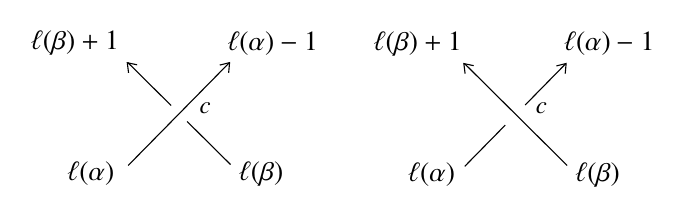
\begin{tikzpicture}[x=0.75pt,y=0.75pt,yscale=-1,xscale=1]	
			\draw    (339.04,32.33) -- (388.49,81.42) ;
			\draw    (225.66,32.01) -- (176.99,81.45) ;
			\draw    (176.89,31.91) -- (197.71,52.56) ;
			\draw   (177.19,36.8) -- (176.57,31.94) -- (181.32,32.93) ;
			\draw   (221.15,33.05) -- (225.86,31.9) -- (225.42,36.77) ;
			\draw    (205.39,60.22) -- (226.34,81) ;
			\draw   (339.33,37.22) -- (338.72,32.36) -- (343.47,33.34) ;
			\draw   (383.3,33.47) -- (388.01,32.31) -- (387.57,37.19) ;
			\draw    (387.8,32.42) -- (368.27,52.3) ;
			\draw    (358.67,62) -- (339.14,81.87) ;
			\draw (210.22,50) node [anchor=north west][inner sep=0.75pt]  [font=\small]  {$c$};
			\draw (372.22,50) node [anchor=north west][inner sep=0.75pt]  [font=\small]  {$c$};
			\draw (146.49,78.53) node [anchor=north west][inner sep=0.75pt]  [font=\normalsize]  {$\ell(\alpha)$};
			\draw (229.1,78.57) node [anchor=north west][inner sep=0.75pt]  [font=\normalsize]  {$\ell(\beta)$};
			\draw (128.85,15.31) node [anchor=north west][inner sep=0.75pt]  [font=\normalsize]  {$\ell(\beta)+1$};
			\draw (223.6,15.75) node [anchor=north west][inner sep=0.75pt]  [font=\normalsize]  {$\ell(\alpha)-1$};
			\draw (310.64,78.95) node [anchor=north west][inner sep=0.75pt]  [font=\normalsize]  {$\ell(\alpha)$};
			\draw (391.25,78.98) node [anchor=north west][inner sep=0.75pt]  [font=\normalsize]  {$\ell(\beta)$};
			\draw (294,15.73) node [anchor=north west][inner sep=0.75pt]  [font=\normalsize]  {$\ell(\beta)+1$};
			\draw (385.74,15.75) node [anchor=north west][inner sep=0.75pt]  [font=\normalsize]  {$\ell(\alpha)-1$};
		\end{tikzpicture}
		\caption{Labeling around a classical crossing $c$ of $D$.} \label{fig11}
	\end{center}
\end{figure}
For a classical crossing $c$ of $D$, let $\ell(\alpha)$ and $\ell(\beta)$ denote the labels of the incoming arcs $\alpha$ and $\beta$, respectively. The \textit{weight} of $c$ is denoted by $W_D(c)$ and defined by
$$
W_D(c) = \operatorname{sgn}(c)\,\big(\ell(\alpha) - (\ell(\beta)+1)\big),
$$
where $\operatorname{sgn}(c)$ is the sign of the crossing. 

The parity of classical crossings in virtual knotoid diagrams is defined in the same way as for virtual knots, see~\cite{Man}. We recall the definition adapted to our setting.

Let $D$ be an oriented virtual knotoid diagram and let $c$ be a classical crossing of $D$. Consider the diagram obtained by applying the orientation-preserving smoothing, also known as  $1$-smoothing, at the crossing $c$. This operation produces a two-component diagram, denoted by $D_1 \cup D_2$. An ordering ($D_1, D_2$) for components $D_1$ and $D_2$ of $D_1 \cup D_2$ is chosen according to the sign of $c$ as shown in Fig.~\ref{fig12}. Let $I(c)$ denote the number of classical crossings between the two components $D_1$ and $D_2$. If $I(c)$ is even, then the crossing $c$ is called \textit{even}, otherwise, it is called \textit{odd}.  This definition is independent of the choice of orientation. We note that this parity is the same as parity of the degree $d(c)$ of crossing $c$ considered in~\cite{FLV}. 
\begin{figure}[!ht]
	\begin{center}
		\tikzset{every picture/.style={line width=1.0pt}}  
		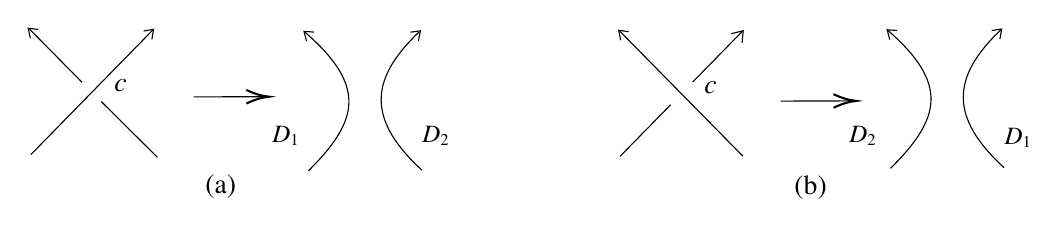
\begin{tikzpicture}[x=0.75pt,y=0.75pt,yscale=-1,xscale=1]	
			\draw    (154.26,40.4) -- (95.17,100.78) ;
			\draw   (149.49,41.25) -- (154.28,40.44) -- (153.47,45.3) ;
			\draw    (129.09,75.23) -- (156.09,102.06) ;
			\draw    (438.11,41.26) -- (414.06,65.8) ;
			\draw    (378.9,41.33) -- (438.23,101.57) ;
			\draw   (432.64,42.53) -- (438.36,41.12) -- (437.83,47.08) ;
			\draw    (403.39,76.8) -- (379.02,101.64) ;
			\draw    (94.17,40.01) -- (119.76,65.9) ;
			\draw    (228.89,108.6) .. controls (253.17,84.5) and (257.06,67.8) .. (227.37,41.93) ;
			\draw    (282.27,41.65) .. controls (257.88,64.79) and (257.34,84.13) .. (283.57,108.32) ; 
			\draw    (509.35,107.4) .. controls (533.64,83.3) and (537.53,66.6) .. (507.84,40.73) ; 
			\draw    (562.73,40.45) .. controls (538.34,63.59) and (537.8,82.93) .. (564.04,107.12) ;
			\draw    (173.55,72.98) -- (207.91,72.9) ;
			\draw [shift={(209.9,72.9)}, rotate = 179.87] [color={rgb, 255:red, 0; green, 0; blue, 0 }  ][line width=0.75]    (10.93,-3.29) .. controls (6.95,-1.4) and (3.31,-0.3) .. (0,0) .. controls (3.31,0.3) and (6.95,1.4) .. (10.93,3.29)   ;
			\draw   (278.04,41.81) -- (282.85,41.15) -- (281.9,45.98) ;
			\draw   (558.09,41.05) -- (562.89,40.28) -- (562.04,45.14) ;
			\draw   (512.57,41.03) -- (507.73,40.65) -- (508.96,45.42) ;
			\draw   (383.21,41.58) -- (378.4,40.89) -- (379.33,45.73) ;
			\draw   (231.59,41.78) -- (226.75,41.4) -- (227.98,46.17) ;
			\draw   (98.71,40.52) -- (93.89,39.91) -- (94.89,44.74) ;
			\draw    (456.42,75.01) -- (490.78,74.93) ;
			\draw [shift={(492.78,74.93)}, rotate = 179.87] [color={rgb, 255:red, 0; green, 0; blue, 0 }  ][line width=0.75]    (10.93,-3.29) .. controls (6.95,-1.4) and (3.31,-0.3) .. (0,0) .. controls (3.31,0.3) and (6.95,1.4) .. (10.93,3.29)   ;
			\draw (134.17,63) node [anchor=north west][inner sep=0.75pt]    {$c$};
			\draw (418.4,64) node [anchor=north west][inner sep=0.75pt]    {$c$};
			\draw (178,109.2) node [anchor=north west][inner sep=0.75pt]    {(a)};
			\draw (461.8,109.8) node [anchor=north west][inner sep=0.75pt]    {(b)};
			\draw (210,85.65) node [anchor=north west][inner sep=0.75pt]  [font=\small]  {$D_{1}$};
			\draw (562.73,86.65) node [anchor=north west][inner sep=0.75pt]  [font=\small]  {$D_{1}$};
			\draw (282.27,85.65) node [anchor=north west][inner sep=0.75pt]  [font=\small]  {$D_{2}$};
			\draw (488,85.65) node [anchor=north west][inner sep=0.75pt]  [font=\small]  {$D_{2}$};
		\end{tikzpicture}
		\caption{Applying the orientation-preserving smoothing at the crossing $c$.} \label{fig12} 
	\end{center}
\end{figure}

The intersection index of an ordered virtual multi-knotoid associated with a smoothed crossing $c$ in virtual knotoid diagrams is defined in the same way as for virtual knots, see~\cite[Def 3.1]{Hen}. We now present the definition adjusted for virtual knotoids. The intersection index $i(c)$ is given by $i(c) = \sum_{e \in D_1 \cap D_2} \operatorname{ind}(e)$, where $\operatorname{ind}(e)$ is defined for classical crossings $e \in D_1 \cap D_2$ as shown in Fig.~\ref{fig511}. In case (a), when $D_1$ is over, we suppose $\operatorname{ind}(e)=\operatorname{sgn}(e)$; \and in case (b), when $D_2$ is over, we suppose $\operatorname{ind}(e)=-\operatorname{sgn}(e)$. 

\begin{figure}[htbp]
	\begin{center}
		\tikzset{every picture/.style={line width=1.0pt}} 
		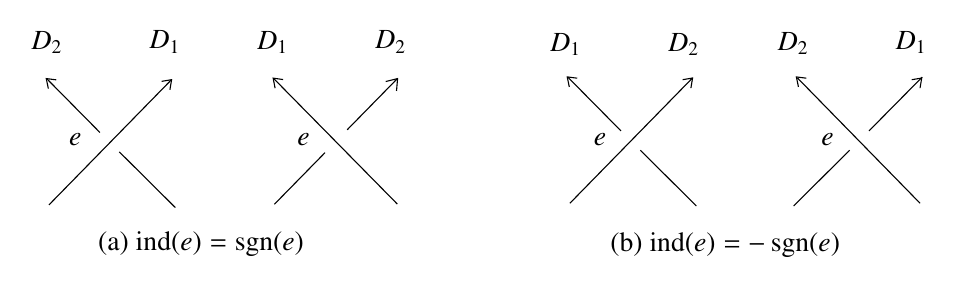
\begin{tikzpicture}[x=0.75pt,y=0.75pt,yscale=-1,xscale=1]
			\draw    (153.66,169.2) -- (94.57,229.58) ;
			\draw   (148.89,170.05) -- (153.68,169.24) -- (152.87,174.1) ; 
			\draw    (128.49,204.03) -- (155.49,230.86) ;
			\draw    (93.57,168.81) -- (119.16,194.7) ;
			\draw   (98.11,169.32) -- (93.29,168.71) -- (94.29,173.54) ;
			\draw    (404.66,168.4) -- (345.57,228.78) ;
			\draw   (399.89,169.25) -- (404.68,168.44) -- (403.87,173.3) ;
			\draw    (379.49,203.23) -- (406.49,230.06) ;
			\draw    (344.57,168.01) -- (370.16,193.9) ;
			\draw   (349.11,168.52) -- (344.29,167.91) -- (345.29,172.74) ;
			\draw    (262.31,168.86) -- (238.26,193.4) ;
			\draw    (203.1,168.93) -- (262.43,229.17) ;
			\draw   (256.84,170.13) -- (262.56,168.72) -- (262.03,174.68) ;
			\draw    (227.59,204.4) -- (203.22,229.24) ;
			\draw   (207.41,169.18) -- (202.6,168.49) -- (203.53,173.33) ;
			\draw    (455.2,168.4) -- (514.29,228.78) ;
			\draw   (510.29,169.25) -- (515.08,168.44) -- (514.27,173.3) ;
			\draw    (480.37,203.23) -- (453.37,230.06) ;
			\draw    (515.29,168.01) -- (489.7,193.9) ;
			\draw   (459.51,168.52) -- (454.69,167.91) -- (455.69,172.74) ;
			\draw (334.6,145.8) node [anchor=north west][inner sep=0.75pt]    {$D_{1}$};
			\draw (391.47,145.65) node [anchor=north west][inner sep=0.75pt]    {$D_{2}$};
			\draw (444.2,145) node [anchor=north west][inner sep=0.75pt]    {$D_{2}$};
			\draw (501.07,144.85) node [anchor=north west][inner sep=0.75pt]    {$D_{1}$};
			\draw (193.4,144.6) node [anchor=north west][inner sep=0.75pt]    {$D_{1}$};
			\draw (250.27,144.45) node [anchor=north west][inner sep=0.75pt]    {$D_{2}$};
			\draw (84.6,144.6) node [anchor=north west][inner sep=0.75pt]    {$D_{2}$};
			\draw (141.47,144.45) node [anchor=north west][inner sep=0.75pt]    {$D_{1}$};
			\draw (103.02,194) node [anchor=north west][inner sep=0.75pt]    {$e$};
			\draw (213.02,194) node [anchor=north west][inner sep=0.75pt]    {$e$};
			\draw (355.82,194) node [anchor=north west][inner sep=0.75pt]    {$e$};
			\draw (465.44,194) node [anchor=north west][inner sep=0.75pt]    {$e$};
			\draw (117,241.2) node [anchor=north west][inner sep=0.75pt]    {(a) $\operatorname{ind}(e)=\operatorname{sgn}(e)$};
			\draw (363.8,241.8) node [anchor=north west][inner sep=0.75pt]    {(b) $\operatorname{ind}(e)=-\operatorname{sgn}(e)$};
		\end{tikzpicture}
		\caption{The $\operatorname{ind}(e)$ for $e \in D_1 \cap D_2$.} \label{fig511}
	\end{center}
\end{figure}

Let $D$ be an oriented knotoid diagram. Denote by $C(D)$ the set of classical crossings of $D$. Using the parity of crossings, we split $C(D)$ into two subsets: the set $O(D)$ of odd crossings and the set $E(D)$ of even crossings. Clearly, $C(D) = O(D) \cup E(D)$ is a disjoint union. Moreover, both sets $O(D)$ and $E(D)$ are invariant under reversing the orientation of $D$.

In \cite[Thm. 2.6]{Lee}, Lee presented an invariant of virtual knots. We extend its parity-enhanced form to virtual knotoids. 

\begin{definition} \label{def2.1}
	{\rm 
		With the above notation, \textit{the two-variable parity polynomial} $\mathbf{P}_D(x,y) \in \mathbb Z[x^{\pm 1}, y^{\pm 1}]$ of $D$ is defined by	
		$$
		\mathbf{P}_D(x,y)=\sum_{c \in E(D)} \operatorname{sgn}(c) i(c) x^{W_D(c)} + \sum_{c \in O(D)} \operatorname{sgn}(c) i(c) y^{W_D(c)}. 
		$$
	}
\end{definition}

\begin{theorem} \label{th2.1}
	Let $K$ be a virtual knotoid with diagram $D$. Then $\mathbf{P}_D(x,y)$ is an invariant of $K$.
\end{theorem}

\begin{proof}
	Let $D'$ be an oriented diagram of $K$ obtained from $D$ by applying one $M$-move, where $M$ belongs to the set of generalized Reidemeister moves. We consider the following moves.
	
	\noindent
	\textbf{Case (i):} $M =\Omega_1$. Assume that $c^*$ is the new classical crossing generated by the $\Omega_1$-move and $C(D')=C(D)\cup \{c^*\}$. Let $\alpha$ be an arc of $D$ with its integer labeling $\ell(\alpha)$, and  $\alpha_1, \alpha_2, \alpha_3$ be three arcs in $D'$ corresponding to $\alpha$. Then, from Fig.~\ref{fig1122}, the integer labels are  $\ell(\alpha_1) = \ell(\alpha)$, $\ell(\alpha_2) = \ell(\alpha)+1$, $\ell(\alpha_3) = \ell(\alpha)$. For any other arc $\gamma$ of $D$, denote by $\gamma'$ its corresponding arc in $D'$, then $\ell(\gamma') =  \ell(\gamma)$. Moreover, $W_{D'}(c^*)=0$, regardless of whether $\operatorname{sgn}(c^*)=1$ or $\operatorname{sgn}(c^*)=-1$. Obviously, $I(c^*)=0$ and $i(c^*)=0$. The set of odd crossings remains unchanged, while the new crossing $c^*$ is even. Thus, $O(D') = O(D)$ and $E(D') = E(D) \cup \{c^*\}$. 
	\begin{figure}[!ht]
		\begin{center}
			\tikzset{every picture/.style={line width=1.0pt}}  
			\begin{tikzpicture}[x=0.75pt,y=0.75pt,yscale=-1,xscale=1]	
				\draw    (188.51,242.37) .. controls (188.45,201.75) and (124.57,201.96) .. (124.83,242.58) ;
				\draw    (358.43,225.98) .. controls (303.62,180.58) and (471.22,202.41) .. (331.55,244.72) ;
				\draw    (371.6,236.78) .. controls (379.23,243.58) and (388.79,248.5) .. (400.94,250.73) ;
				\draw    (549.39,227.26) .. controls (604.51,182.22) and (436.77,202.94) .. (576.15,246.17) ;
				\draw    (536.15,237.97) .. controls (528.47,244.72) and (518.88,249.58) .. (506.72,251.72) ;
				\draw    (236.26,226.03) -- (286.48,225.69) ;
				\draw [shift={(288.48,225.68)}, rotate = 179.62] [color={rgb, 255:red, 0; green, 0; blue, 0 }  ][line width=0.75]    (10.93,-3.29) .. controls (6.95,-1.4) and (3.31,-0.3) .. (0,0) .. controls (3.31,0.3) and (6.95,1.4) .. (10.93,3.29)   ;
				\draw [shift={(234.26,226.04)}, rotate = 359.62] [color={rgb, 255:red, 0; green, 0; blue, 0 }  ][line width=0.75]    (10.93,-3.29) .. controls (6.95,-1.4) and (3.31,-0.3) .. (0,0) .. controls (3.31,0.3) and (6.95,1.4) .. (10.93,3.29)   ;
				\draw   (397.09,246.85) -- (401.14,250.66) -- (396,252.73) ;
				\draw   (572.71,241.87) -- (576.13,246.26) -- (570.73,247.51) ;
				\draw   (191.47,238.41) -- (188.4,243.05) -- (185.49,238.33) ;
				\draw (448.33,210.67) node [anchor=north west][inner sep=0.75pt]   [align=left] {or};
				\draw (353.67,234) node [anchor=north west][inner sep=0.75pt]    [font=\small]  {$c^{*}$};
				\draw (534.33,236) node [anchor=north west][inner sep=0.75pt]    [font=\small]  {$c^{*}$};
				\draw (107,236.67) node [anchor=north west][inner sep=0.75pt]    {$\alpha $};
				\draw (311.33,243) node [anchor=north west][inner sep=0.75pt]    {$\alpha _{1}$};
				\draw (355.33,188) node [anchor=north west][inner sep=0.75pt]    {$\alpha _{2}$};
				\draw (579,246) node [anchor=north west][inner sep=0.75pt]    {$\alpha _{3}$};
				\draw (489,246) node [anchor=north west][inner sep=0.75pt]    {$\alpha _{1}$};
				\draw (529,188.67) node [anchor=north west][inner sep=0.75pt]    {$\alpha _{2}$};
				\draw (402.67,248) node [anchor=north west][inner sep=0.75pt]    {$\alpha _{3}$};
			\end{tikzpicture}
			\caption{$\Omega_1$-move.} \label{fig1122}
		\end{center}
	\end{figure}
	
	Let $c\in C(D)$ be any classical crossing of $D$, and $c'\in C(D')$ the classical crossing of $D'$ corresponding to $c$. It is clear that $\operatorname{sgn}(c)=\operatorname{sgn}(c')$, and $W_D(c)=W_{D'}(c')$. Then $i(c^*)=0$ implies 
	$$
	\mathbf{P}_{D'}(x,y) - \mathbf{P}_D(x,y) = \operatorname{sgn}(c^*)i(c^*)x^0 =0.
	$$
	
	\noindent
	\textbf{Case (ii):} $M =\Omega_2$. Assume that $c_1$, $c_2$ are the new classical crossings generated by the $\Omega_2$-move and $C(D')=C(D)\cup \{c_1,c_2\}$. Let $\alpha$ and $\beta$ be arcs in $D$ with  integer labels $\ell(\alpha)$ and $\ell(\beta)$, respectively.  Denote the corresponding six arcs in $D'$ by $\alpha_1, \alpha_2, \alpha_3$ and $\beta_1, \beta_2, \beta_3$.  Then, from Fig.~\ref{fig1133} we get the integer labels $\ell(\alpha_1) = \ell(\alpha)$, $\ell(\alpha_2) = \ell(\alpha) - 1$, $\ell(\alpha_3) = \ell(\alpha)$ and $\ell(\beta_1) = \ell(\beta)$, $\ell(\beta_2) = \ell(\beta) + 1$, $\ell(\beta_3) = \ell(\beta)$. 
	For any other arc $\gamma$ of $D$, denote by $\gamma'$ its corresponding arc in $D'$, we have $\ell(\gamma') = \ell(\gamma)$. Moreover, $W_{D'}(c_1)=W_{D'}(c_2)=\ell(\beta)-\ell(\alpha)+1$. Since $I(c_1)=I(c_2)$, see Fig.~\ref{fig2233}, the crossings $c_1$ and $c_2$ have the same parity, that is, either $c_1, c_2 \in O(D')$ or $c_1, c_2 \in E(D')$. Equivalently, $\bigl(O(D'), E(D')\bigr) = \bigl(O(D) \cup \{c_1, c_2\}, E(D)\bigr)$ or $\bigl(O(D'), E(D')\bigr) = \bigl(O(D), E(D) \cup \{c_1, c_2\}\bigr)$. Moreover, $\operatorname{sgn}(c_1)=- \operatorname{sgn}(c_2)$ and $i(c_1)=i(c_2)$.
	
	\begin{figure}[!ht]
		\begin{center}
			\tikzset{every picture/.style={line width=1.0pt}}  
			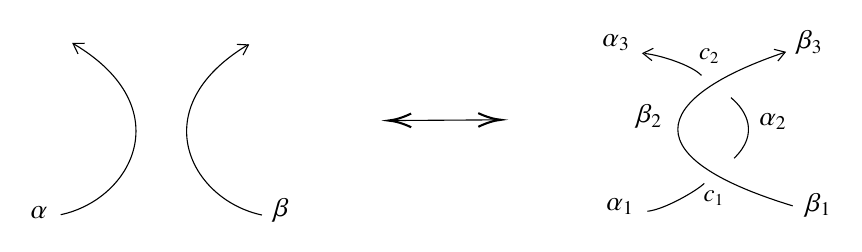
\begin{tikzpicture}[x=0.75pt,y=0.75pt,yscale=-1,xscale=1]		
				\draw    (441.35,405.47) .. controls (357.73,379.88) and (379.24,351.14) .. (437.51,331.5) ;
				\draw    (371.37,408.07) .. controls (379.43,407.31) and (395.05,398.27) .. (398.76,394.64) ;
				\draw    (411.59,353.32) .. controls (419.23,359.66) and (425.32,370.81) .. (413.12,382.51) ;
				\draw    (370.19,332.07) .. controls (377.2,332.81) and (392.49,337.49) .. (397.42,342.64) ;
				\draw    (88.68,409.73) .. controls (123.38,402.34) and (146.12,357.94) .. (95.2,327.59) ;
				\draw    (248.59,364.36) -- (298.81,364.03) ;
				\draw [shift={(300.81,364.01)}, rotate = 179.62] [color={rgb, 255:red, 0; green, 0; blue, 0 }  ][line width=0.75]    (10.93,-3.29) .. controls (6.95,-1.4) and (3.31,-0.3) .. (0,0) .. controls (3.31,0.3) and (6.95,1.4) .. (10.93,3.29)   ;
				\draw [shift={(246.59,364.37)}, rotate = 359.62] [color={rgb, 255:red, 0; green, 0; blue, 0 }  ][line width=0.75]    (10.93,-3.29) .. controls (6.95,-1.4) and (3.31,-0.3) .. (0,0) .. controls (3.31,0.3) and (6.95,1.4) .. (10.93,3.29)   ;
				\draw    (185.62,409.88) .. controls (150.92,402.49) and (128.18,358.09) .. (179.1,327.74) ;
				\draw   (97.03,332.24) -- (94.62,327.22) -- (100.17,327.15) ;
				\draw   (432.32,330.06) -- (437.72,331.41) -- (434.23,335.72) ;
				\draw   (373.54,335.49) -- (369.22,331.99) -- (374.2,329.55) ;
				\draw   (173.53,327.66) -- (179.09,327.93) -- (176.52,332.84) ;
				\draw (397.23,396.68) node [anchor=north west][inner sep=0.75pt]  [font=\small,rotate=-0.11]  {$c_{1}$};
				\draw (394.99,328.57) node [anchor=north west][inner sep=0.75pt]  [font=\small,rotate=-0.11]  {$c_{2}$};
				\draw (73.04,404.27) node [anchor=north west][inner sep=0.75pt]  [font=\normalsize]  {$\alpha $};
				\draw (190.33,400.43) node [anchor=north west][inner sep=0.75pt]  [font=\normalsize]  {$\beta $};
				\draw (424.15,359.45) node [anchor=north west][inner sep=0.75pt]  [font=\normalsize,rotate=-0.11]  {$\alpha _{2}$};
				\draw (348.52,321.36) node [anchor=north west][inner sep=0.75pt]  [font=\normalsize,rotate=-0.11]  {$\alpha _{3}$};
				\draw (350.48,400.47) node [anchor=north west][inner sep=0.75pt]  [font=\normalsize,rotate=-0.11]  {$\alpha _{1}$};
				\draw (442.57,319.89) node [anchor=north west][inner sep=0.75pt]  [font=\normalsize,rotate=-0.11]  {$\beta _{3}$};
				\draw (365.31,355.5) node [anchor=north west][inner sep=0.75pt]  [font=\normalsize,rotate=-0.11]  {$\beta _{2}$};
				\draw (446.75,398.14) node [anchor=north west][inner sep=0.75pt]  [font=\normalsize,rotate=-0.11]  {$\beta _{1}$};	
			\end{tikzpicture}
			\caption{$\Omega_2$-move.} \label{fig1133}
		\end{center}
	\end{figure}
	
	\begin{figure}[!ht]
		\begin{center}
			\tikzset{every picture/.style={line width=1.0pt}}  
			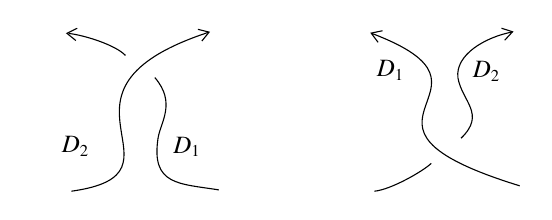
\begin{tikzpicture}[x=0.75pt,y=0.75pt,yscale=-1,xscale=1]	
				\draw    (419.35,125.79) .. controls (320.03,95.22) and (420.88,79.93) .. (348.19,52.4) ;
				\draw    (349.37,128.39) .. controls (357.43,127.63) and (373.05,118.6) .. (376.76,114.96) ;
				\draw    (389.59,73.65) .. controls (391.45,85.08) and (403.32,91.13) .. (391.12,102.84) ;
				\draw    (389.59,73.65) .. controls (388.31,62.79) and (402.3,54.3) .. (415.86,51.65) ;
				\draw   (410.63,49.87) -- (415.92,51.58) -- (412.15,55.65) ;
				\draw   (351.14,56.68) -- (347.82,52.21) -- (353.25,51.09) ;
				\draw    (203.37,128.39) .. controls (265.32,119.77) and (182.58,80.33) .. (269.51,51.82) ;
				\draw    (245.12,102.84) .. controls (241.7,125.63) and (255.23,124.66) .. (274.43,127.77) ;
				\draw    (243.59,73.65) .. controls (254.03,85.86) and (246.3,95.16) .. (245.12,102.84) ;
				\draw    (202.19,52.4) .. controls (209.2,53.14) and (224.49,57.81) .. (229.42,62.97) ;
				\draw   (264.32,50.39) -- (269.72,51.74) -- (266.23,56.05) ;
				\draw   (205.54,55.82) -- (201.22,52.32) -- (206.2,49.88) ;
				\draw (251,101) node [anchor=north west][inner sep=0.75pt]  [font=\small]  {$D_{1}$};
				\draw (197.27,100.65) node [anchor=north west][inner sep=0.75pt]  [font=\small]  {$D_{2}$};
				\draw (349,64) node [anchor=north west][inner sep=0.75pt] [font=\small]   {$D_{1}$};
				\draw (395.27,64.65) node [anchor=north west][inner sep=0.75pt]  [font=\small]  {$D_{2}$};
			\end{tikzpicture}
			\caption{The diagrams obtained by orientation-preserving smoothing at $c_1$ and $c_2$.} \label{fig2233}
		\end{center}
	\end{figure}
	
	Let $c\in C(D)$ be any classical crossing of $D$, and $c'\in C(D')$ the classical crossing of $D'$ corresponding to $c$. It is clear that $\operatorname{sgn}(c)=\operatorname{sgn}(c')$ and $W_D(c)=W_{D'}(c')$. Then
	\begin{flalign*}
		&\mathbf{P}_{D'}(x,y)-\mathbf{P}_D(x,y) = \\
		&\begin{cases}
			\operatorname{sgn}(c_1)i(c_1)x^{\ell(\beta)-\ell(\alpha)+1} + \operatorname{sgn}(c_2)i(c_2)x^{\ell(\beta)-\ell(\alpha)+1} = 0, & \text{if } c_1,c_2\in E(D),\\[6pt]
			\operatorname{sgn}(c_1)i(c_1)y^{\ell(\beta)-\ell(\alpha)+1} + \operatorname{sgn}(c_2)i(c_2)y^{\ell(\beta)-\ell(\alpha)+1} = 0, & \text{if } c_1,c_2\in O(D).
		\end{cases}
	\end{flalign*}
	The case of $\Omega_2$ when $\beta$ has the opposite orientation can be shown in a similar way.
	
	\noindent
	\textbf{Case (iii):} $M =\Omega_3$. Assume that $c_1, c_2,c_3\in D$ are the classical crossings involved in $\Omega_3$-move. Denote by $c'_1, c'_2,c'_3$ the corresponding crossings in $D'$. Let $\alpha_1$, $\alpha_2$, $\alpha_3$, $\beta_1$, $\beta_2$, $\beta_3$, $\delta_1$, $\delta_2$, and $\delta_3$ be nine arcs of $D$, participating in the $\Omega_3$-move. Let $\alpha'_1$, $\alpha'_2$, $\alpha'_3$, $\beta'_1$, $\beta'_2$, $\beta'_3$, $\delta'_1$, $\delta'_2$, and $\delta'_3$ be the corresponding arcs in $D'$. For any other arc $\gamma$ of $D$, denote by $\gamma'$ its corresponding arc in $D'$. It is easy to see that  $\ell(\gamma') = \ell(\gamma)$. 
	\begin{figure}[!ht]
		\begin{center}
			\tikzset{every picture/.style={line width=1.0pt}}  
			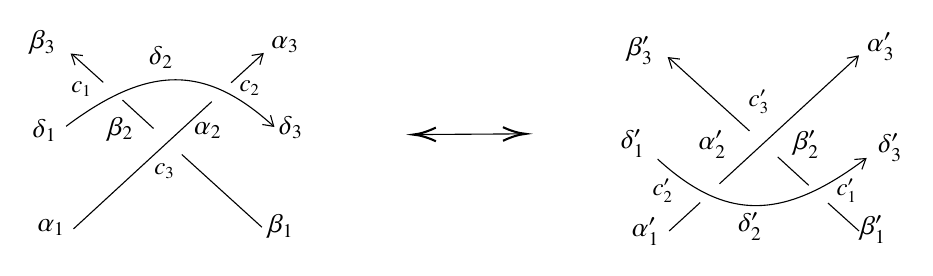
\begin{tikzpicture}[x=0.75pt,y=0.75pt,yscale=-1,xscale=1]	
				\draw    (153.24,488.05) -- (86.62,549.38) ;
				\draw    (138.78,513.53) -- (177.4,548.59) ;
				\draw    (110.25,487.34) -- (125.17,501) ;
				\draw    (86.04,465.34) -- (100.96,478.79) ;
				\draw    (162.54,479) -- (177.47,465.34) ;
				\draw    (83.04,499.96) .. controls (123.04,469.96) and (150.45,470.19) .. (183.04,499.96) ;
				\draw    (397.84,527.66) -- (464.46,466.34) ; 
				\draw    (412.3,502.19) -- (373.68,467.13) ;
				\draw    (440.83,528.38) -- (425.91,514.72) ;
				\draw    (465.04,550.37) -- (450.12,536.93) ;
				\draw    (388.54,536.71) -- (373.61,550.38) ;
				\draw    (468.04,515.76) .. controls (428.04,545.76) and (400.63,545.53) .. (368.04,515.76) ;
				\draw    (252.26,503.93) -- (302.48,503.6) ;
				\draw [shift={(304.48,503.59)}, rotate = 179.62] [color={rgb, 255:red, 0; green, 0; blue, 0 }  ][line width=0.75]    (10.93,-3.29) .. controls (6.95,-1.4) and (3.31,-0.3) .. (0,0) .. controls (3.31,0.3) and (6.95,1.4) .. (10.93,3.29)   ;
				\draw [shift={(250.26,503.95)}, rotate = 359.62] [color={rgb, 255:red, 0; green, 0; blue, 0 }  ][line width=0.75]    (10.93,-3.29) .. controls (6.95,-1.4) and (3.31,-0.3) .. (0,0) .. controls (3.31,0.3) and (6.95,1.4) .. (10.93,3.29)   ;
				\draw   (181.54,494.62) -- (183.06,499.97) -- (177.58,499.09) ;
				\draw   (87.34,470.48) -- (85.63,465.19) -- (91.13,465.86) ;
				\draw   (172.44,465.8) -- (177.94,464.94) -- (176.41,470.27) ;
				\draw   (466.46,520.71) -- (468.39,515.49) -- (462.86,515.93) ;
				\draw   (374.96,472.18) -- (373.25,466.89) -- (378.75,467.56) ;
				\draw   (459.24,467.14) -- (464.7,466.07) -- (463.37,471.45) ;
				\draw (68.13,543.54) node [anchor=north west][inner sep=0.75pt]    {$\alpha _{1}$};
				\draw (143.62,496.71) node [anchor=north west][inner sep=0.75pt]    {$\alpha _{2}$};
				\draw (180.8,455.21) node [anchor=north west][inner sep=0.75pt]    {$\alpha _{3}$};
				\draw (179.47,541.38) node [anchor=north west][inner sep=0.75pt]    {$\beta _{1}$};
				\draw (102.29,494.55) node [anchor=north west][inner sep=0.75pt]    {$\beta _{2}$};
				\draw (64.8,452.71) node [anchor=north west][inner sep=0.75pt]    {$\beta _{3}$};
				\draw (65.8,495.38) node [anchor=north west][inner sep=0.75pt]    {$\delta _{1}$};
				\draw (121.96,460.22) node [anchor=north west][inner sep=0.75pt]    {$\delta _{2}$};
				\draw (184.47,493.71) node [anchor=north west][inner sep=0.75pt]    {$\delta _{3}$};
				\draw (354.51,542.54) node [anchor=north west][inner sep=0.75pt]    {$\alpha'_{1}$};
				\draw (386.66,500.71) node [anchor=north west][inner sep=0.75pt]    {$\alpha'_{2}$};
				\draw (467.84,453.54) node [anchor=north west][inner sep=0.75pt]    {$\alpha'_{3}$};
				\draw (464.84,541.71) node [anchor=north west][inner sep=0.75pt]    {$\beta'_{1}$};
				\draw (432.66,500.55) node [anchor=north west][inner sep=0.75pt]    {$\beta'_{2}$};
				\draw (352.51,455.38) node [anchor=north west][inner sep=0.75pt]    {$\beta'_{3}$};
				\draw (349.17,500.04) node [anchor=north west][inner sep=0.75pt]    {$\delta'_{1}$};
				\draw (405.66,540.22) node [anchor=north west][inner sep=0.75pt]    {$\delta'_{2}$};
				\draw (473.17,502.04) node [anchor=north west][inner sep=0.75pt]    {$\delta'_{3}$};
				\draw (84.33,477.04) node [anchor=north west][inner sep=0.75pt]    [font=\small] {$c_{1}$};
				\draw (124.33,516.5) node [anchor=north west][inner sep=0.75pt]    [font=\small] {$c_{3}$};
				\draw (165.33,476.83) node [anchor=north west][inner sep=0.75pt]    [font=\small] {$c_{2}$};
				\draw (453,523.83) node [anchor=north west][inner sep=0.75pt]    [font=\small] {$c'_{1}$};
				\draw (410.67,480.83) node [anchor=north west][inner sep=0.75pt]    [font=\small] {$c'_{3}$};
				\draw (364.33,523.83) node [anchor=north west][inner sep=0.75pt]    [font=\small] {$c'_{2}$};
			\end{tikzpicture}
			\caption{$\Omega_3$-move.} \label{fig1144}
		\end{center}
	\end{figure}
	
	From Fig.~\ref{fig1144}, we have 
	\begin{equation}
		\operatorname{sgn}(c'_i)=\operatorname{sgn}(c_i), \label{2.2}
	\end{equation}
	where $i=1,2,3$. Moreover, for $D$ we have 
	$$
	\begin{gathered}
		\ell(\alpha_2)=\ell(\alpha_1)-1, \quad \ell(\alpha_3)=\ell(\alpha_1), \quad 
		\ell(\beta_2)=\ell(\beta_1)+1,  \cr 
		\ell(\beta_3)=\ell(\beta_1)+2, \quad  \ell(\delta_2)=\ell(\delta_1)-1, \quad
		\ell(\delta_3)=\ell(\delta_1)-2, 
	\end{gathered}
	$$
	and for $D'$ we have
	$$
	\begin{gathered}	
		\ell(\alpha'_1)=\ell(\alpha_1), \quad 
		\ell(\alpha'_2)=\ell(\alpha_1)+1, \quad  
		\ell(\alpha'_3)=\ell(\alpha_1), \cr 
		\ell(\beta'_1)=\ell(\beta_1), \quad
		\ell(\beta'_2)=\ell(\beta_1)+1, \quad   
		\ell(\beta'_3)=\ell(\beta_1)+2, \cr
		\ell(\delta'_1)=\ell(\delta_1), \quad 
		\ell(\delta'_2)=\ell(\delta_1)-1, \quad 
		\ell(\delta'_3)=\ell(\delta_1)-2.
	\end{gathered}
	$$
	Therefore,
	\begin{align}
		W_{D'}(c'_1) &= W_D(c_1) = \ell(\delta_1)-\ell(\beta_1)-2, \label{2.3} \\
		W_{D'}(c'_2) &= W_D(c_2) = \ell(\delta_1)-\ell(\alpha_1)-1, \label{2.4} \\
		W_{D'}(c'_3) &= W_D(c_3) = \ell(\alpha_1)-\ell(\beta_1)-1.  \label{2.5} 
	\end{align}
	
	\begin{figure}[!ht]
		\centering
		\tikzset{every picture/.style={line width=1.0pt}}  
		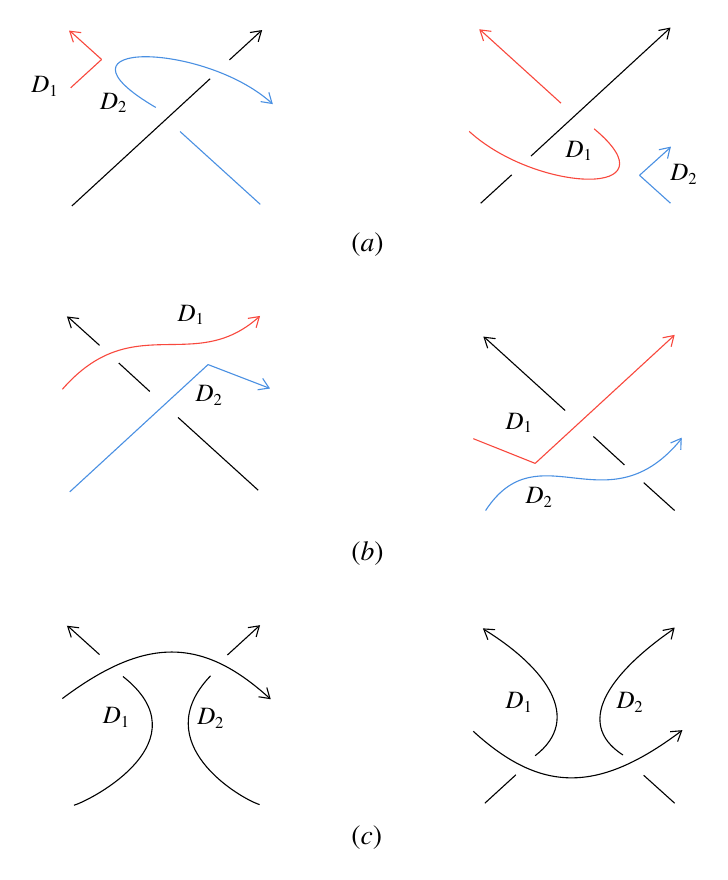
\begin{tikzpicture}[x=0.75pt,y=0.75pt,yscale=-1.0,xscale=1.0]	
			\draw    (114.24,269.68) -- (47.62,331) ;
			\draw [color={rgb, 255:red, 74; green, 144; blue, 226 }  ,draw opacity=1 ]   (99.78,295.15) -- (138.4,330.21) ;
			\draw [color={rgb, 255:red, 248; green, 72; blue, 61 }  ,draw opacity=1 ]   (61.96,260.41) -- (47.03,274.08) ;
			\draw [color={rgb, 255:red, 248; green, 72; blue, 61 }  ,draw opacity=1 ]   (47.04,246.97) -- (61.96,260.41) ;
			\draw    (123.54,260.63) -- (138.47,246.96) ;
			\draw [color={rgb, 255:red, 74; green, 144; blue, 226 }  ,draw opacity=1 ]   (88.04,283.52) .. controls (32.04,250.72) and (111.45,251.82) .. (144.04,281.58) ;
			\draw  [color={rgb, 255:red, 74; green, 144; blue, 226 }  ,draw opacity=1 ] (142.54,276.24) -- (144.06,281.59) -- (138.58,280.71) ;
			\draw  [color={rgb, 255:red, 248; green, 72; blue, 61 }  ,draw opacity=1 ] (48.34,252.1) -- (46.63,246.81) -- (52.13,247.48) ;
			\draw   (133.44,247.42) -- (138.94,246.56) -- (137.41,251.89) ;
			\draw    (268.84,306.95) -- (335.46,245.63) ;
			\draw [color={rgb, 255:red, 248; green, 72; blue, 61 }  ,draw opacity=1 ]   (283.3,281.48) -- (244.68,246.42) ;
			\draw [color={rgb, 255:red, 74; green, 144; blue, 226 }  ,draw opacity=1 ]   (336.04,329.66) -- (321.12,316.22) ;
			\draw    (259.54,316) -- (244.61,329.67) ;
			\draw [color={rgb, 255:red, 248; green, 72; blue, 61 }  ,draw opacity=1 ]   (299.24,293.81) .. controls (339.24,327.15) and (271.63,324.81) .. (239.04,295.05) ;
			\draw  [color={rgb, 255:red, 74; green, 144; blue, 226 }  ,draw opacity=1 ] (334.62,308.17) -- (335.86,302.75) -- (330.44,303.9) ;
			\draw  [color={rgb, 255:red, 248; green, 72; blue, 61 }  ,draw opacity=1 ] (245.96,251.47) -- (244.25,246.17) -- (249.75,246.85) ;
			\draw   (330.24,246.43) -- (335.7,245.36) -- (334.37,250.74) ;
			\draw [color={rgb, 255:red, 74; green, 144; blue, 226 }  ,draw opacity=1 ]   (321.12,316.22) -- (336.04,302.77) ;
			\draw    (46.04,533.7) -- (60.96,547.15) ;
			\draw    (122.54,547.36) -- (137.47,533.7) ;
			\draw    (43.04,568.32) .. controls (83.04,538.32) and (110.45,538.55) .. (143.04,568.32) ;
			\draw    (338.04,618.73) -- (323.12,605.28) ;
			\draw    (261.54,605.07) -- (246.61,618.73) ;
			\draw    (341.04,584.11) .. controls (301.04,614.11) and (273.63,613.88) .. (241.04,584.11) ;
			\draw   (141.54,562.97) -- (143.06,568.33) -- (137.58,567.45) ;
			\draw   (47.34,538.83) -- (45.63,533.54) -- (51.13,534.21) ;
			\draw   (132.44,534.15) -- (137.94,533.29) -- (136.41,538.62) ;
			\draw   (339.46,589.06) -- (341.39,583.84) -- (335.86,584.29) ;
			\draw   (248.08,539.98) -- (246.05,534.79) -- (251.59,535.14) ;
			\draw   (332.24,535.49) -- (337.7,534.43) -- (336.37,539.81) ;
			\draw    (72.25,557.69) .. controls (111.51,588.59) and (57.51,617.05) .. (48.62,619.73) ;
			\draw    (114.45,557.36) .. controls (83.17,589.93) and (129.19,616.71) .. (138.07,619.4) ;
			\draw    (246.68,535.32) .. controls (276.3,553.72) and (293.9,578.12) .. (270.84,595.85) ;
			\draw    (337.33,534.99) .. controls (309.83,553.93) and (287.9,579.32) .. (313.17,595.52) ;
			\draw [color={rgb, 255:red, 74; green, 144; blue, 226 }  ,draw opacity=1 ]   (113.24,407.41) -- (46.62,468.73) ;
			\draw    (98.78,432.88) -- (137.4,467.94) ;
			\draw    (70.25,406.69) -- (85.17,420.36) ;
			\draw    (46.04,384.7) -- (60.96,398.15) ;
			\draw [color={rgb, 255:red, 74; green, 144; blue, 226 }  ,draw opacity=1 ]   (113.24,407.41) -- (142.65,418.74) ;
			\draw [color={rgb, 255:red, 248; green, 72; blue, 61 }  ,draw opacity=1 ]   (43.04,419.32) .. controls (76.99,380.41) and (106.32,412.41) .. (137.47,384.7) ;
			\draw [color={rgb, 255:red, 248; green, 72; blue, 61 }  ,draw opacity=1 ]   (270.84,455.02) -- (337.46,393.7) ;
			\draw    (285.3,429.55) -- (246.68,394.49) ;
			\draw    (313.83,455.73) -- (298.91,442.07) ;
			\draw    (338.04,477.73) -- (323.12,464.28) ;
			\draw [color={rgb, 255:red, 74; green, 144; blue, 226 }  ,draw opacity=1 ]   (341.37,443.11) .. controls (305.72,487.03) and (272.72,438.37) .. (246.95,477.73) ;
			\draw  [color={rgb, 255:red, 74; green, 144; blue, 226 }  ,draw opacity=1 ] (139.57,414.08) -- (142.63,418.73) -- (137.14,419.54) ;
			\draw   (47.34,389.83) -- (45.63,384.54) -- (51.13,385.21) ;
			\draw  [color={rgb, 255:red, 248; green, 72; blue, 61 }  ,draw opacity=1 ] (132.44,385.15) -- (137.94,384.29) -- (136.41,389.62) ;
			\draw  [color={rgb, 255:red, 74; green, 144; blue, 226 }  ,draw opacity=1 ] (341,448.55) -- (341.18,442.99) -- (336.08,445.17) ;
			\draw   (247.96,399.53) -- (246.25,394.24) -- (251.75,394.91) ;
			\draw  [color={rgb, 255:red, 248; green, 72; blue, 61 }  ,draw opacity=1 ] (332.24,394.49) -- (337.7,393.43) -- (336.37,398.81) ;
			\draw [color={rgb, 255:red, 248; green, 72; blue, 61 }  ,draw opacity=1 ]   (270.84,455.02) -- (241.04,443.11) ;
			\draw (181,342.91) node [anchor=north west][inner sep=0.75pt]    {$(a)$};
			\draw (181,628.51) node [anchor=north west][inner sep=0.75pt]    {$(c)$};
			\draw (26.6,267.35) node [anchor=north west][inner sep=0.75pt]  [font=\small]  {$D_{1}$};
			\draw (59.67,275.2) node [anchor=north west][inner sep=0.75pt]  [font=\small]  {$D_{2}$};
			\draw (284,298.35) node [anchor=north west][inner sep=0.75pt]  [font=\small]  {$D_{1}$};
			\draw (334.47,309.8) node [anchor=north west][inner sep=0.75pt]  [font=\small]  {$D_{2}$};
			\draw (61,571.35) node [anchor=north west][inner sep=0.75pt]  [font=\small]  {$D_{1}$};
			\draw (255.08,563.9) node [anchor=north west][inner sep=0.75pt]  [font=\small]  {$D_{1}$};
			\draw (106.47,571.8) node [anchor=north west][inner sep=0.75pt]  [font=\small]  {$D_{2}$};
			\draw (308.47,563.9) node [anchor=north west][inner sep=0.75pt]  [font=\small]  {$D_{2}$};
			\draw (181,491.51) node [anchor=north west][inner sep=0.75pt]    {$(b)$};
			\draw (97,377.35) node [anchor=north west][inner sep=0.75pt]  [font=\small]  {$D_{1}$};
			\draw (255,429.35) node [anchor=north west][inner sep=0.75pt]  [font=\small]  {$D_{1}$};
			\draw (105.67,416.2) node [anchor=north west][inner sep=0.75pt]  [font=\small]  {$D_{2}$};
			\draw (264.67,465.2) node [anchor=north west][inner sep=0.75pt]  [font=\small]  {$D_{2}$};	
		\end{tikzpicture}
		\caption{(a) Orientation-preserving smoothings at crossings $c_1$ and $c'_1$. (b) Orientation-preserving smoothings at crossings $c_2$ and $c'_2$.(c) Orientation-preserving smoothings at crossings $c_3$ and $c'_3$.} \label{fig2244}
	\end{figure}
	
	Let us discuss the parity of crossings $c_i$ and $c'_i$, where $i=1, 2, 3$. For $c_1$ and $c'_1$, consider the diagrams obtained by applying the orientation-preserving smoothings at $c_1$ and $c'_1$, respectively, see Fig.~\ref{fig2244}(a). Then there are two cases:
	\begin{itemize}
		\item[{(1)}] If the red part belongs to one component, say $D_1$, and the blue and black parts belong to the other component , say $D_2$, then $I(c'_1) - I(c_1) = 2$;
		\item[{(2)}] If the blue part belongs to one component, say $D_2$, and the red and black parts belong to the other, say $D_1$, then $I(c'_1) - I(c_1) = -2$.
	\end{itemize}
	
	For $c_2$ and $c'_2$, consider the diagrams obtained by applying the orientation-preserving smoothings at $c_2$ and $c'_2$, respectively, see Fig.~\ref{fig2244}(b). Then there are two cases:
	\begin{itemize}
		\item[{(1)}] If the red part belongs to one component, say $D_1$, and the blue and black parts belong to the other component , say $D_2$, then $I(c'_2) - I(c_2) = 0$;
		\item[{(2)}] If the blue part belongs to one component, say $D_2$, and the red and black parts belong to the other, say $D_1$, then $I(c'_2) - I(c_2) = 0$.
	\end{itemize}
	
	For $c_3$ and $c'_3$, from Fig.~\ref{fig2244}(c), one can easily obtain $I(c'_3) = I(c_3)$. Therefore, crossings $c'_i$ and $c_i$ have the same parity, for $i=1, 2, 3$. Moreover, $i(c'_i) = i(c_i)$ for $i=1, 2, 3$. Combining formulas \eqref{2.2}--\eqref{2.5}, we obtain that the contribution of $c'_i$ in $\mathbf{P}_{D'}(x,y)$ is the same as that of $c_i$ in $\mathbf{P}_{D}(x,y)$, where $i=1, 2, 3$. 
	
	Let $c\in C(D)$ be any classical crossing of $D$ not involved in $\Omega_3$-move, and $c'\in C(D')$ the classical crossing of $D'$ corresponding to $c$. It is clear that $\operatorname{sgn}(c)=\operatorname{sgn}(c')$ and $W_D(c)=W_{D'}(c')$. Therefore, the contribution of $c$ in $\mathbf{P}_D(x,y)$ is the same as that of $c'$ in $\mathbf{P}_{D'}(x,y)$. Hence, $\mathbf{P}_{D'}(x,y)=\mathbf{P}_D(x,y).$ The oriented $\Omega_3$-move has eight possible orientation configurations. Up to simultaneous reversal of all orientations, these reduce to four distinct cases. The remaining three cases can be proved individually by the same method.
	
	\noindent
	\textbf{Case (iv):} $M = \Omega^{m}_3$. The classical crossings involved in $\Omega^{m}_3$ remain unchanged, so this move has no effect on $\mathbf{P}_D(x,y)$. Hence $\mathbf{P}_{D'}(x,y) = \mathbf{P}_D(x,y)$.
	
	\noindent
	\textbf{Case (v):} $M = \Omega^{v}_i$ $(i=1,2,3)$ or $M = \Omega_v$. These moves do not involve classical crossings, so they have no effect on the definition of $\mathbf{P}_D(x,y)$. Hence, $\mathbf{P}_{D'}(x,y)=\mathbf{P}_D(x,y)$.
	
	It follows from the above cases that $\mathbf{P}_D(x,y)$ is an invariant of an oriented virtual knotoid $K$.
\end{proof}
Thus, for a virtual knotoid $K$ with diagram $D$, we may write $\mathbf{P}_K(x,y)=\mathbf{P}_D(x,y)$. 

\begin{remark}
	{\rm
		The invariant $P_K(x,y)$ is defined using the sign of classical crossing together with the parity of crossing, and the computation of $P_K(x,y)$ requires a single traversal of all crossings in a virtual knotoid diagram. Therefore, the overall computational complexity is linear in the number of classical crossings.
	}	
\end{remark}

\subsection{An example of calculation of $\mathbf{P}_K(x,y)$}

The following example shows that the invariant $\mathbf{P}(x,y)$ is non-trivial. 
\begin{example} \label{exp2.1}{\rm
		Consider the virtual knotoid $K_+$, whose diagram $D_+$ is presented in Fig.~\ref{fig1119} (a).  The diagram $D_+$ contains two virtual crossings and four classical crossings $c_1$, $c_2$, $c_3$ and $c_+$.  We will demonstrate that $\mathbf{P}_{D_+}(x,y) \neq 0$. 
		\begin{figure}[!ht]
			\begin{center}
				\tikzset{every picture/.style={line width=1.0pt}}  
				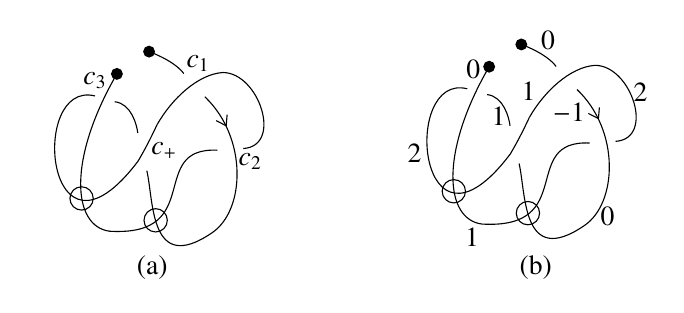
\begin{tikzpicture}[x=0.75pt,y=0.75pt,yscale=-0.85,xscale=0.85]	
					\draw    (144.72,101.18) .. controls (154.23,102.16) and (157.28,114.59) .. (157.77,118.86) ;
					\draw    (162.91,140.27) .. controls (166.93,157.69) and (164.49,199.46) .. (199.76,175.52) ; 
					\draw    (157.95,134.8) .. controls (105.46,204.41) and (95.68,88.39) .. (133.53,97.89) ; 
					\draw    (145.94,85.38) .. controls (117.92,133.68) and (120.53,171.93) .. (141.94,174.58) ;
					\draw    (141.94,174.58) .. controls (196.24,177.63) and (162.84,126.75) .. (202.88,128.64) ;
					\draw    (217.56,127.69) .. controls (240.24,126.27) and (226.48,84.67) .. (206.01,84.6) ; 
					\draw    (195.76,98.34) .. controls (220.22,121.54) and (218.71,162.91) .. (199.76,175.52) ;
					\draw    (168.76,114.09) .. controls (177.08,99.49) and (191.84,85.55) .. (206.01,84.6) ;
					\draw    (164.18,72.76) .. controls (166.85,73.71) and (178.86,78.45) .. (183.87,85.23) ;
					\draw    (157.95,134.8) .. controls (163.24,125.82) and (166.34,119.12) .. (168.76,114.09) ; 
					\draw   (119.31,155.97) .. controls (119.31,152.32) and (122.27,149.37) .. (125.92,149.37) .. controls (129.57,149.37) and (132.52,152.32) .. (132.52,155.97) .. controls (132.52,159.62) and (129.57,162.58) .. (125.92,162.58) .. controls (122.27,162.58) and (119.31,159.62) .. (119.31,155.97) -- cycle ;
					\draw   (161.31,168.37) .. controls (161.31,164.72) and (164.27,161.77) .. (167.92,161.77) .. controls (171.57,161.77) and (174.52,164.72) .. (174.52,168.37) .. controls (174.52,172.02) and (171.57,174.98) .. (167.92,174.98) .. controls (164.27,174.98) and (161.31,172.02) .. (161.31,168.37) -- cycle ;
					\draw  [fill={rgb, 255:red, 0; green, 0; blue, 0 }  ,fill opacity=1 ] (142.9,85.38) .. controls (142.9,83.7) and (144.26,82.34) .. (145.94,82.34) .. controls (147.62,82.34) and (148.98,83.7) .. (148.98,85.38) .. controls (148.98,87.06) and (147.62,88.42) .. (145.94,88.42) .. controls (144.26,88.42) and (142.9,87.06) .. (142.9,85.38) -- cycle ;
					\draw  [fill={rgb, 255:red, 0; green, 0; blue, 0 }  ,fill opacity=1 ] (161.14,72.76) .. controls (161.14,71.09) and (162.5,69.73) .. (164.18,69.73) .. controls (165.85,69.73) and (167.21,71.09) .. (167.21,72.76) .. controls (167.21,74.44) and (165.85,75.8) .. (164.18,75.8) .. controls (162.5,75.8) and (161.14,74.44) .. (161.14,72.76) -- cycle ;
					\draw   (208.43,108.41) -- (207.87,114.79) -- (202.18,111.86) ;
					\draw    (355.72,97.11) .. controls (365.23,98.09) and (368.28,110.52) .. (368.77,114.79) ;
					\draw    (373.91,136.2) .. controls (377.93,153.62) and (375.49,195.39) .. (410.76,171.45) ;
					\draw    (368.95,130.73) .. controls (316.46,200.34) and (306.68,84.32) .. (344.53,93.82) ; 
					\draw    (356.94,81.31) .. controls (328.92,129.61) and (331.53,167.86) .. (352.94,170.51) ;
					\draw    (352.94,170.51) .. controls (407.24,173.56) and (373.84,122.68) .. (413.88,124.57) ;
					\draw    (428.56,123.62) .. controls (451.24,122.2) and (437.48,80.6) .. (417.01,80.53) ;
					\draw    (406.76,94.27) .. controls (431.22,117.47) and (429.71,158.84) .. (410.76,171.45) ; 
					\draw    (379.76,110.02) .. controls (388.08,95.42) and (402.84,81.48) .. (417.01,80.53) ;
					\draw    (375.18,68.69) .. controls (377.85,69.64) and (389.86,74.38) .. (394.87,81.16) ;
					\draw    (368.95,130.73) .. controls (374.24,121.75) and (377.34,115.05) .. (379.76,110.02) ;
					\draw   (330.31,151.9) .. controls (330.31,148.25) and (333.27,145.3) .. (336.92,145.3) .. controls (340.57,145.3) and (343.52,148.25) .. (343.52,151.9) .. controls (343.52,155.55) and (340.57,158.51) .. (336.92,158.51) .. controls (333.27,158.51) and (330.31,155.55) .. (330.31,151.9) -- cycle ;
					\draw   (372.31,164.3) .. controls (372.31,160.65) and (375.27,157.7) .. (378.92,157.7) .. controls (382.57,157.7) and (385.52,160.65) .. (385.52,164.3) .. controls (385.52,167.95) and (382.57,170.91) .. (378.92,170.91) .. controls (375.27,170.91) and (372.31,167.95) .. (372.31,164.3) -- cycle ;
					\draw  [fill={rgb, 255:red, 0; green, 0; blue, 0 }  ,fill opacity=1 ] (353.9,81.31) .. controls (353.9,79.63) and (355.26,78.27) .. (356.94,78.27) .. controls (358.62,78.27) and (359.98,79.63) .. (359.98,81.31) .. controls (359.98,82.99) and (358.62,84.35) .. (356.94,84.35) .. controls (355.26,84.35) and (353.9,82.99) .. (353.9,81.31) -- cycle ;
					\draw  [fill={rgb, 255:red, 0; green, 0; blue, 0 }  ,fill opacity=1 ] (372.14,68.69) .. controls (372.14,67.02) and (373.5,65.66) .. (375.18,65.66) .. controls (376.85,65.66) and (378.21,67.02) .. (378.21,68.69) .. controls (378.21,70.37) and (376.85,71.73) .. (375.18,71.73) .. controls (373.5,71.73) and (372.14,70.37) .. (372.14,68.69) -- cycle ;
					\draw   (419.43,104.34) -- (418.87,110.72) -- (413.18,107.79) ;
					\draw (164.01,122.84) node [anchor=north west][inner sep=0.75pt]    {$c_+$};
					\draw (155.73,187.18) node [anchor=north west][inner sep=0.75pt]    {(a)};
					\draw (184,73.07) node [anchor=north west][inner sep=0.75pt]    {$c_{1}$};
					\draw (213.5,129.07) node [anchor=north west][inner sep=0.75pt]    {$c_{2}$};
					\draw (125.5,83.07) node [anchor=north west][inner sep=0.75pt]    {$c_{3}$};
					\draw (372.73,187.18) node [anchor=north west][inner sep=0.75pt]    {(b)};
					\draw (384.88,59.5) node [anchor=north west][inner sep=0.75pt]    {$0$};
					\draw (437.38,88.79) node [anchor=north west][inner sep=0.75pt]    {$2$};
					\draw (356.81,102.93) node [anchor=north west][inner sep=0.75pt]    {$1$};
					\draw (391.88,100.64) node [anchor=north west][inner sep=0.75pt]    {$-1$};
					\draw (342.53,76.21) node [anchor=north west][inner sep=0.75pt]    {$0$};
					\draw (341.81,171.07) node [anchor=north west][inner sep=0.75pt]    {$1$};
					\draw (418.67,159.36) node [anchor=north west][inner sep=0.75pt]    {$0$};
					\draw (309.24,123.5) node [anchor=north west][inner sep=0.75pt]    {$2$};
					\draw (373.81,88.21) node [anchor=north west][inner sep=0.75pt]    {$1$};
				\end{tikzpicture}
				\caption{A virtual knotoid diagram $D_+$ and its integer labeling.} \label{fig1119}
			\end{center}
		\end{figure}  
		
		As can be seen from Fig.~\ref{fig1119}(a), $\operatorname{sgn}(c_1)=\operatorname{sgn}(c_2) =-1$ and $ \operatorname{sgn}(c_3) = \operatorname{sgn}(c_+)= 1$.
		\begin{figure}[!ht]
			\begin{center}
				\tikzset{every picture/.style={line width=1.0pt}}  
				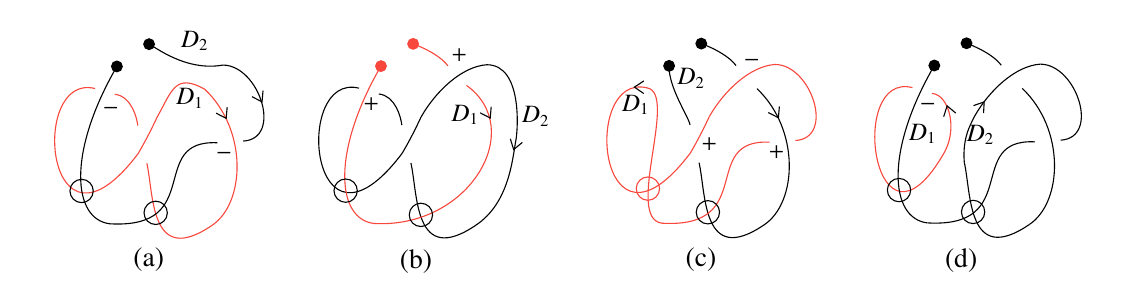
\begin{tikzpicture}[x=0.75pt,y=0.75pt,yscale=-0.85,xscale=0.85]	
					\draw    (204.55,71.94) .. controls (214.06,72.92) and (217.12,85.35) .. (217.61,89.62) ; 
					\draw    (222.74,111.04) .. controls (226.76,128.46) and (224.32,170.22) .. (259.6,146.29) ;
					\draw    (217.78,105.56) .. controls (165.3,175.17) and (155.51,59.15) .. (193.36,68.66) ;
					\draw [color={rgb, 255:red, 248; green, 72; blue, 61 }  ,draw opacity=1 ]   (205.77,56.14) .. controls (177.75,104.44) and (180.36,142.7) .. (201.77,145.34) ;
					\draw [color={rgb, 255:red, 248; green, 72; blue, 61 }  ,draw opacity=1 ]   (201.77,145.34) .. controls (256.07,148.39) and (288.61,91.74) .. (254.27,67.08) ;
					\draw    (282.27,98.08) .. controls (283.27,93.08) and (286.31,55.44) .. (265.84,55.36) ;
					\draw    (282.27,98.08) .. controls (280.27,108.74) and (278.54,133.68) .. (259.6,146.29) ;
					\draw    (228.59,84.85) .. controls (236.92,70.26) and (251.68,56.31) .. (265.84,55.36) ;
					\draw [color={rgb, 255:red, 248; green, 72; blue, 61 }  ,draw opacity=1 ]   (224.01,43.53) .. controls (226.68,44.47) and (238.69,49.21) .. (243.71,55.99) ;
					\draw    (217.78,105.56) .. controls (223.07,96.58) and (226.18,89.88) .. (228.59,84.85) ;
					\draw   (179.15,126.73) .. controls (179.15,123.09) and (182.1,120.13) .. (185.75,120.13) .. controls (189.4,120.13) and (192.36,123.09) .. (192.36,126.73) .. controls (192.36,130.38) and (189.4,133.34) .. (185.75,133.34) .. controls (182.1,133.34) and (179.15,130.38) .. (179.15,126.73) -- cycle ;
					\draw   (221.81,140.47) .. controls (221.81,136.82) and (224.77,133.86) .. (228.42,133.86) .. controls (232.07,133.86) and (235.02,136.82) .. (235.02,140.47) .. controls (235.02,144.12) and (232.07,147.07) .. (228.42,147.07) .. controls (224.77,147.07) and (221.81,144.12) .. (221.81,140.47) -- cycle ;
					\draw  [color={rgb, 255:red, 248; green, 72; blue, 61 }  ,draw opacity=1 ][fill={rgb, 255:red, 248; green, 72; blue, 61 }  ,fill opacity=1 ] (202.74,56.14) .. controls (202.74,54.47) and (204.1,53.11) .. (205.77,53.11) .. controls (207.45,53.11) and (208.81,54.47) .. (208.81,56.14) .. controls (208.81,57.82) and (207.45,59.18) .. (205.77,59.18) .. controls (204.1,59.18) and (202.74,57.82) .. (202.74,56.14) -- cycle ;
					\draw  [color={rgb, 255:red, 248; green, 72; blue, 61 }  ,draw opacity=1 ][fill={rgb, 255:red, 248; green, 72; blue, 61 }  ,fill opacity=1 ] (220.97,43.53) .. controls (220.97,41.85) and (222.33,40.49) .. (224.01,40.49) .. controls (225.69,40.49) and (227.05,41.85) .. (227.05,43.53) .. controls (227.05,45.2) and (225.69,46.56) .. (224.01,46.56) .. controls (222.33,46.56) and (220.97,45.2) .. (220.97,43.53) -- cycle ;
					\draw   (268.26,79.18) -- (267.7,85.56) -- (262.01,82.62) ;
					\draw [color={rgb, 255:red, 248; green, 72; blue, 61 }  ,draw opacity=1 ]   (54.88,72.12) .. controls (64.4,73.11) and (67.45,85.53) .. (67.94,89.8) ;
					\draw [color={rgb, 255:red, 248; green, 72; blue, 61 }  ,draw opacity=1 ]   (73.07,111.22) .. controls (77.1,128.64) and (74.65,170.41) .. (109.93,146.47) ;
					\draw [color={rgb, 255:red, 248; green, 72; blue, 61 }  ,draw opacity=1 ]   (68.12,105.74) .. controls (15.63,175.35) and (5.84,59.34) .. (43.7,68.84) ;
					\draw    (56.11,56.32) .. controls (28.08,104.63) and (30.69,142.88) .. (52.1,145.52) ;
					\draw    (52.1,145.52) .. controls (106.4,148.57) and (73.01,97.69) .. (113.04,99.59) ;
					\draw    (127.72,98.64) .. controls (150.41,97.22) and (136.64,55.62) .. (116.17,55.55) ;
					\draw [color={rgb, 255:red, 248; green, 72; blue, 61 }  ,draw opacity=1 ]   (105.93,69.28) .. controls (130.39,92.48) and (128.87,133.86) .. (109.93,146.47) ;
					\draw [color={rgb, 255:red, 248; green, 72; blue, 61 }  ,draw opacity=1 ]   (78.92,85.03) .. controls (87.25,70.44) and (88.94,59.71) .. (105.93,69.28) ;
					\draw    (74.34,43.71) .. controls (77.01,44.66) and (94.94,59.38) .. (116.17,55.55) ; 
					\draw [color={rgb, 255:red, 248; green, 72; blue, 61 }  ,draw opacity=1 ]   (68.12,105.74) .. controls (73.41,96.76) and (76.51,90.06) .. (78.92,85.03) ;
					\draw   (29.48,126.92) .. controls (29.48,123.27) and (32.44,120.31) .. (36.09,120.31) .. controls (39.73,120.31) and (42.69,123.27) .. (42.69,126.92) .. controls (42.69,130.56) and (39.73,133.52) .. (36.09,133.52) .. controls (32.44,133.52) and (29.48,130.56) .. (29.48,126.92) -- cycle ;
					\draw   (71.48,139.32) .. controls (71.48,135.67) and (74.44,132.71) .. (78.09,132.71) .. controls (81.73,132.71) and (84.69,135.67) .. (84.69,139.32) .. controls (84.69,142.96) and (81.73,145.92) .. (78.09,145.92) .. controls (74.44,145.92) and (71.48,142.96) .. (71.48,139.32) -- cycle ;
					\draw  [fill={rgb, 255:red, 0; green, 0; blue, 0 }  ,fill opacity=1 ] (53.07,56.32) .. controls (53.07,54.65) and (54.43,53.29) .. (56.11,53.29) .. controls (57.78,53.29) and (59.14,54.65) .. (59.14,56.32) .. controls (59.14,58) and (57.78,59.36) .. (56.11,59.36) .. controls (54.43,59.36) and (53.07,58) .. (53.07,56.32) -- cycle ;
					\draw  [fill={rgb, 255:red, 0; green, 0; blue, 0 }  ,fill opacity=1 ] (71.31,43.71) .. controls (71.31,42.03) and (72.67,40.67) .. (74.34,40.67) .. controls (76.02,40.67) and (77.38,42.03) .. (77.38,43.71) .. controls (77.38,45.39) and (76.02,46.75) .. (74.34,46.75) .. controls (72.67,46.75) and (71.31,45.39) .. (71.31,43.71) -- cycle ;
					\draw   (118.6,79.36) -- (118.04,85.74) -- (112.34,82.81) ;
					\draw   (138.93,70.02) -- (138.37,76.41) -- (132.68,73.47) ;
					\draw [color={rgb, 255:red, 248; green, 72; blue, 61 }  ,draw opacity=1 ]   (518.22,71.61) .. controls (527.73,72.59) and (532.64,91.08) .. (525.3,104.74) ;
					\draw    (536.41,110.7) .. controls (540.43,128.12) and (537.99,169.89) .. (573.26,145.95) ;
					\draw [color={rgb, 255:red, 248; green, 72; blue, 61 }  ,draw opacity=1 ]   (525.3,104.74) .. controls (485.64,174.74) and (469.18,58.82) .. (507.03,68.32) ;
					\draw    (519.44,55.81) .. controls (491.42,104.11) and (494.03,142.36) .. (515.44,145.01) ;
					\draw    (515.44,145.01) .. controls (569.74,148.06) and (536.34,97.18) .. (576.38,99.07) ;
					\draw    (591.06,98.12) .. controls (613.74,96.7) and (599.98,55.1) .. (579.51,55.03) ;
					\draw    (569.26,68.77) .. controls (593.72,91.97) and (592.21,133.34) .. (573.26,145.95) ;
					\draw    (542.26,84.52) .. controls (550.58,69.92) and (565.34,55.98) .. (579.51,55.03) ;
					\draw    (537.68,43.19) .. controls (540.35,44.14) and (552.36,48.88) .. (557.37,55.66) ;
					\draw    (536.41,110.7) .. controls (535.3,96.74) and (539.84,89.55) .. (542.26,84.52) ;
					\draw   (492.81,126.4) .. controls (492.81,122.75) and (495.77,119.8) .. (499.42,119.8) .. controls (503.07,119.8) and (506.02,122.75) .. (506.02,126.4) .. controls (506.02,130.05) and (503.07,133.01) .. (499.42,133.01) .. controls (495.77,133.01) and (492.81,130.05) .. (492.81,126.4) -- cycle ;
					\draw   (534.81,138.8) .. controls (534.81,135.15) and (537.77,132.2) .. (541.42,132.2) .. controls (545.07,132.2) and (548.02,135.15) .. (548.02,138.8) .. controls (548.02,142.45) and (545.07,145.41) .. (541.42,145.41) .. controls (537.77,145.41) and (534.81,142.45) .. (534.81,138.8) -- cycle ;
					\draw  [fill={rgb, 255:red, 0; green, 0; blue, 0 }  ,fill opacity=1 ] (516.4,55.81) .. controls (516.4,54.13) and (517.76,52.77) .. (519.44,52.77) .. controls (521.12,52.77) and (522.48,54.13) .. (522.48,55.81) .. controls (522.48,57.49) and (521.12,58.85) .. (519.44,58.85) .. controls (517.76,58.85) and (516.4,57.49) .. (516.4,55.81) -- cycle ;
					\draw  [fill={rgb, 255:red, 0; green, 0; blue, 0 }  ,fill opacity=1 ] (534.64,43.19) .. controls (534.64,41.52) and (536,40.16) .. (537.68,40.16) .. controls (539.35,40.16) and (540.71,41.52) .. (540.71,43.19) .. controls (540.71,44.87) and (539.35,46.23) .. (537.68,46.23) .. controls (536,46.23) and (534.64,44.87) .. (534.64,43.19) -- cycle ;
					\draw    (369.11,55.99) .. controls (368.65,68.31) and (380.45,85.2) .. (380.94,89.47) ;
					\draw    (386.07,110.89) .. controls (390.1,128.31) and (387.65,170.07) .. (422.93,146.13) ;
					\draw [color={rgb, 255:red, 248; green, 72; blue, 61 }  ,draw opacity=1 ]   (381.12,105.41) .. controls (328.63,175.02) and (318.84,59) .. (356.7,68.5) ;
					\draw [color={rgb, 255:red, 248; green, 72; blue, 61 }  ,draw opacity=1 ]   (356.7,68.5) .. controls (374.42,71.77) and (343.69,142.54) .. (365.1,145.19) ;
					\draw [color={rgb, 255:red, 248; green, 72; blue, 61 }  ,draw opacity=1 ]   (365.1,145.19) .. controls (419.4,148.24) and (386.01,97.36) .. (426.04,99.25) ;
					\draw [color={rgb, 255:red, 248; green, 72; blue, 61 }  ,draw opacity=1 ]   (440.72,98.31) .. controls (463.41,96.89) and (449.64,55.29) .. (429.17,55.21) ;
					\draw    (418.93,68.95) .. controls (443.39,92.15) and (441.87,133.53) .. (422.93,146.13) ;
					\draw [color={rgb, 255:red, 248; green, 72; blue, 61 }  ,draw opacity=1 ]   (391.92,84.7) .. controls (400.25,70.11) and (415.01,56.16) .. (429.17,55.21) ;
					\draw    (387.34,43.38) .. controls (390.01,44.32) and (402.02,49.06) .. (407.04,55.84) ;
					\draw [color={rgb, 255:red, 248; green, 72; blue, 61 }  ,draw opacity=1 ]   (381.12,105.41) .. controls (386.41,96.43) and (389.51,89.73) .. (391.92,84.7) ;
					\draw  [color={rgb, 255:red, 248; green, 72; blue, 61 }  ,draw opacity=1 ] (350.48,125.58) .. controls (350.48,121.93) and (353.44,118.98) .. (357.09,118.98) .. controls (360.73,118.98) and (363.69,121.93) .. (363.69,125.58) .. controls (363.69,129.23) and (360.73,132.19) .. (357.09,132.19) .. controls (353.44,132.19) and (350.48,129.23) .. (350.48,125.58) -- cycle ;
					\draw   (384.48,138.98) .. controls (384.48,135.33) and (387.44,132.38) .. (391.09,132.38) .. controls (394.73,132.38) and (397.69,135.33) .. (397.69,138.98) .. controls (397.69,142.63) and (394.73,145.59) .. (391.09,145.59) .. controls (387.44,145.59) and (384.48,142.63) .. (384.48,138.98) -- cycle ;
					\draw  [fill={rgb, 255:red, 0; green, 0; blue, 0 }  ,fill opacity=1 ] (366.07,55.99) .. controls (366.07,54.31) and (367.43,52.95) .. (369.11,52.95) .. controls (370.78,52.95) and (372.14,54.31) .. (372.14,55.99) .. controls (372.14,57.67) and (370.78,59.03) .. (369.11,59.03) .. controls (367.43,59.03) and (366.07,57.67) .. (366.07,55.99) -- cycle ;
					\draw  [fill={rgb, 255:red, 0; green, 0; blue, 0 }  ,fill opacity=1 ] (384.31,43.38) .. controls (384.31,41.7) and (385.67,40.34) .. (387.34,40.34) .. controls (389.02,40.34) and (390.38,41.7) .. (390.38,43.38) .. controls (390.38,45.05) and (389.02,46.41) .. (387.34,46.41) .. controls (385.67,46.41) and (384.31,45.05) .. (384.31,43.38) -- cycle ;
					\draw   (431.6,79.02) -- (431.04,85.41) -- (425.34,82.47) ;
					\draw   (285.94,99.37) -- (280.99,103.44) -- (279.09,97.33) ;
					\draw   (524.74,84.79) -- (526.67,78.68) -- (531.6,82.78) ;
					\draw   (541.63,78.53) -- (547.69,76.44) -- (547.33,82.84) ;
					\draw   (354.71,71.67) -- (349.43,68.05) -- (354.78,64.53) ;
					\draw (88,67.33) node [anchor=north west][inner sep=0.75pt]  [font=\small]  {$D_{1}$};
					\draw (90.67,34.67) node [anchor=north west][inner sep=0.75pt]  [font=\small]  {$D_{2}$};
					\draw (244,76.67) node [anchor=north west][inner sep=0.75pt]  [font=\small]  {$D_{1}$};
					\draw (284,77.33) node [anchor=north west][inner sep=0.75pt]  [font=\small]  {$D_{2}$};
					\draw (536,88) node [anchor=north west][inner sep=0.75pt]  [font=\small]  {$D_{2}$};
					\draw (503.33,87.33) node [anchor=north west][inner sep=0.75pt]  [font=\small]  {$D_{1}$};
					\draw (340.67,71) node [anchor=north west][inner sep=0.75pt]  [font=\small]  {$D_{1}$};
					\draw (372.14,55.99) node [anchor=north west][inner sep=0.75pt]  [font=\small]  {$D_{2}$};
					\draw (110.8,100.4) node [anchor=north west][inner sep=0.75pt]  [font=\small]  {$-$};
					\draw (46.7,74.84) node [anchor=north west][inner sep=0.75pt]  [font=\small]  {$-$};
					\draw (244.2,44.8) node [anchor=north west][inner sep=0.75pt]  [font=\small]  {$+$};
					\draw (194.36,72.66) node [anchor=north west][inner sep=0.75pt]  [font=\small]  {$+$};
					\draw (509.8,72.6) node [anchor=north west][inner sep=0.75pt]  [font=\small]  {$-$};
					\draw (424,99.8) node [anchor=north west][inner sep=0.75pt]  [font=\small]  {$+$};
					\draw (385.94,95.47) node [anchor=north west][inner sep=0.75pt]  [font=\small]  {$+$};
					\draw (410,47.8) node [anchor=north west][inner sep=0.75pt]  [font=\small]  {$-$};
					\draw (64,157.85) node [anchor=north west][inner sep=0.75pt]   [align=left] {(a)};
					\draw (377,157.85) node [anchor=north west][inner sep=0.75pt]   [align=left] {(c)};
					\draw (524,157.85) node [anchor=north west][inner sep=0.75pt]   [align=left] {(d)};
					\draw (215,158.85) node [anchor=north west][inner sep=0.75pt]   [align=left] {(b)};
				\end{tikzpicture}
				\caption{(a)--(d): Diagrams obtained by orientation-preserving smoothing at classical crossings $c_1$, $c_2$, $c_3$ and $c_+$. }  \label{fig13}
			\end{center}
		\end{figure} 
		
		According to Fig.~\ref{fig1119}(b), the straightforward calculations give
		$$
		\begin{aligned}
			W_{D_+}(c_1) &= -(0-2) = 2, \quad W_{D_+}(c_2) =-(2-0)= -2, \\ W_{D_+}(c_3) &=1-2= -1, \quad W_{D_+}(c_+) =2-1= 1.
		\end{aligned}
		$$ 
		From Fig.~\ref{fig13}, we see that $I(c_1)=I(c_2)=2$, $I(c_3)=3$ and $I(c_+)=1$, thus $c_1, c_2 \in E(D_+)$ and $c_3, c_+ \in O(D_+)$. Moreover, $i(c_1)=-2$, $i(c_2)=2$, $i(c_3)=1$, and $i(c_+)=-1$. Therefore, 
		\begin{eqnarray*}
			\mathbf{P}_{D_+}(x,y)&=&\operatorname{sgn}(c_1) i(c_1) x^{W_{D_+}(c_1)}+\operatorname{sgn}(c_2) i(c_2) x^{W_{D_+}(c_2)}\\
			&&+\operatorname{sgn}(c_3) i(c_3) y^{W_{D_+}(c_3)}+\operatorname{sgn}(c_+) i(c_+) y^{W_{D_+}(c_+)}\\
			&=& -(-2) x^{2}-2 x^{-2} + y^{-1} +(-1) y= 2x^2-2x^{-2}+y^{-1}-y \neq 0.
	\end{eqnarray*} }
\end{example} 

%%%%%
\section{The properties of $\mathbf{P}_K(x,y)$} \label{section3}


\subsection{$\mathbf{P}_K(x,y)$ and the odd writhe} \label{subsection3.0}

For a virtual knotoid $K$, the odd writhe invariant introduced in~\cite{GK} is given by
$
J(K)=\sum_{c\in O(K)}\operatorname{sgn}(c),
$
where $O(K)$ denotes the set of odd crossings of $K$. We now exhibit two virtual knotoids $K_1$ and $K_2$ that cannot be distinguished by $J(K)$, while $\mathbf{P}_K(x,y)$ successfully distinguishes them.

\begin{example} \label{example3.0}
	{\rm
		Let $K_1$ and $K_2$ be oriented virtual knotoids with diagrams $D_1$ and $D_2$ presented in Fig.~\ref{fig602}. 
		\begin{figure}[!ht]
			\begin{center}
				\tikzset{every picture/.style={line width=1.pt}}  
				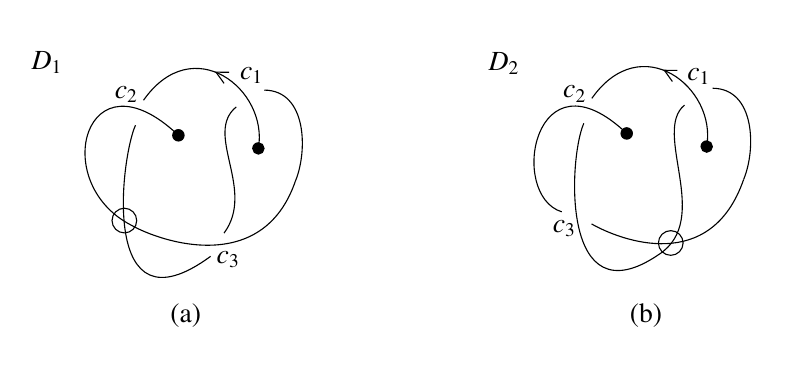
\begin{tikzpicture}[x=0.75pt,y=0.75pt,yscale=-0.9,xscale=0.9]		
					\draw    (131.96,87.54) .. controls (158.32,49.99) and (198.95,81.67) .. (193.46,113.35) ;
					\draw    (125.37,154.41) .. controls (80.55,131.4) and (101.21,59.38) .. (150.63,106.31) ; 
					\draw    (125.37,154.41) .. controls (141.32,163.47) and (195.69,181.71) .. (213.22,130.95) ; 
					\draw    (196.59,82.12) .. controls (219.32,82.22) and (220.02,114.58) .. (213.22,130.95) ;
					\draw    (181.58,91.12) .. controls (164.01,105.59) and (192.27,135.23) .. (175.06,158.7) ;
					\draw    (127.66,100.9) .. controls (119.6,118.89) and (108.39,214.8) .. (167.86,171.1) ;
					\draw  [fill={rgb, 255:red, 0; green, 0; blue, 0 }  ,fill opacity=1 ] (147.59,106.31) .. controls (147.59,104.63) and (148.95,103.27) .. (150.63,103.27) .. controls (152.31,103.27) and (153.67,104.63) .. (153.67,106.31) .. controls (153.67,107.99) and (152.31,109.35) .. (150.63,109.35) .. controls (148.95,109.35) and (147.59,107.99) .. (147.59,106.31) -- cycle ;
					\draw  [fill={rgb, 255:red, 0; green, 0; blue, 0 }  ,fill opacity=1 ] (190.42,113.35) .. controls (190.42,111.67) and (191.78,110.31) .. (193.46,110.31) .. controls (195.13,110.31) and (196.49,111.67) .. (196.49,113.35) .. controls (196.49,115.02) and (195.13,116.38) .. (193.46,116.38) .. controls (191.78,116.38) and (190.42,115.02) .. (190.42,113.35) -- cycle ;
					\draw   (115.1,151.96) .. controls (115.1,148.31) and (118.06,145.35) .. (121.71,145.35) .. controls (125.35,145.35) and (128.31,148.31) .. (128.31,151.96) .. controls (128.31,155.6) and (125.35,158.56) .. (121.71,158.56) .. controls (118.06,158.56) and (115.1,155.6) .. (115.1,151.96) -- cycle ;
					\draw   (175.08,78.51) -- (170.77,72.5) -- (177.73,72.58) ;
					\draw    (371.96,86.54) .. controls (398.32,48.99) and (438.95,80.67) .. (433.46,112.35) ; 
					\draw    (355.84,147.27) .. controls (326.84,138.27) and (341.21,58.38) .. (390.63,105.31) ;
					\draw    (371.84,153.77) .. controls (387.78,162.83) and (435.69,180.71) .. (453.22,129.95) ;
					\draw    (436.59,81.12) .. controls (459.32,81.22) and (460.02,113.58) .. (453.22,129.95) ;
					\draw    (421.58,90.12) .. controls (404.01,104.59) and (436.84,151.27) .. (407.86,170.1) ;
					\draw    (367.66,99.9) .. controls (359.6,117.89) and (354.84,206.27) .. (407.86,170.1) ;
					\draw  [fill={rgb, 255:red, 0; green, 0; blue, 0 }  ,fill opacity=1 ] (387.59,105.31) .. controls (387.59,103.63) and (388.95,102.27) .. (390.63,102.27) .. controls (392.31,102.27) and (393.67,103.63) .. (393.67,105.31) .. controls (393.67,106.99) and (392.31,108.35) .. (390.63,108.35) .. controls (388.95,108.35) and (387.59,106.99) .. (387.59,105.31) -- cycle ;
					\draw  [fill={rgb, 255:red, 0; green, 0; blue, 0 }  ,fill opacity=1 ] (430.42,112.35) .. controls (430.42,110.67) and (431.78,109.31) .. (433.46,109.31) .. controls (435.13,109.31) and (436.49,110.67) .. (436.49,112.35) .. controls (436.49,114.02) and (435.13,115.38) .. (433.46,115.38) .. controls (431.78,115.38) and (430.42,114.02) .. (430.42,112.35) -- cycle ;
					\draw   (407.6,163.96) .. controls (407.6,160.31) and (410.56,157.35) .. (414.21,157.35) .. controls (417.85,157.35) and (420.81,160.31) .. (420.81,163.96) .. controls (420.81,167.6) and (417.85,170.56) .. (414.21,170.56) .. controls (410.56,170.56) and (407.6,167.6) .. (407.6,163.96) -- cycle ;
					\draw   (415.08,77.51) -- (410.77,71.5) -- (417.73,71.58) ;
					\draw (182.24,68.44) node [anchor=north west][inner sep=0.75pt]    {$c_{1}$};
					\draw (115.24,78.44) node [anchor=north west][inner sep=0.75pt]    {$c_{2}$};
					\draw (169.74,166.94) node [anchor=north west][inner sep=0.75pt]    {$c_{3}$};
					\draw (421.74,68.84) node [anchor=north west][inner sep=0.75pt]    {$c_{1}$};
					\draw (355.24,78.34) node [anchor=north west][inner sep=0.75pt]    {$c_{2}$};
					\draw (349.74,150.34) node [anchor=north west][inner sep=0.75pt]    {$c_{3}$};
					\draw (70.24,59.94) node [anchor=north west][inner sep=0.75pt]    {$D_{1}$};
					\draw (314.9,60.44) node [anchor=north west][inner sep=0.75pt]    {$D_{2}$};
					\draw (144.9,194.94) node [anchor=north west][inner sep=0.75pt]    {(a)};
					\draw (390.9,194.94) node [anchor=north west][inner sep=0.75pt]    {(b)};
				\end{tikzpicture}
				\caption{Virtual knotoid diagrams $D_1$ and $D_2$.} \label{fig602}
			\end{center}
		\end{figure} 
		The diagram $D_1$ contains one virtual crossing and three classical crossings $c_1$, $c_2$, and $c_3$. One can see from Fig.~\ref{fig602}(a) that 
		$\operatorname{sgn}(c_1)=\operatorname{sgn}(c_2)=\operatorname{sgn}(c_3)=-1$. 
		\begin{figure}[!ht]
			\begin{center}
				\tikzset{every picture/.style={line width=1.pt}}  
				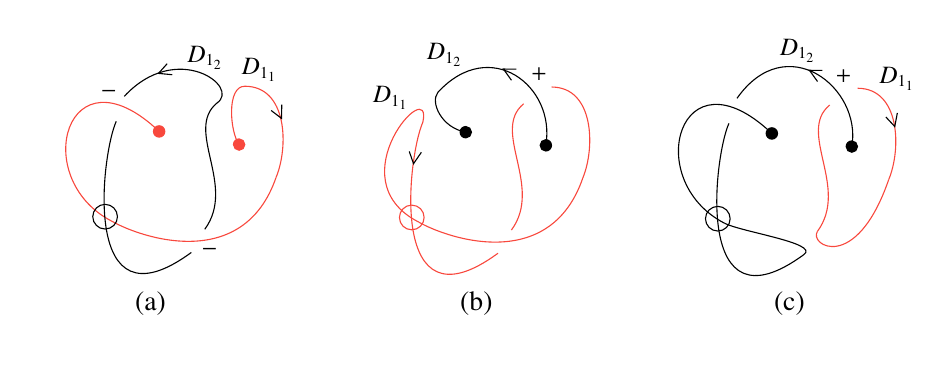
\begin{tikzpicture}[x=0.75pt,y=0.75pt,yscale=-0.9,xscale=0.9]		
					\draw    (74.46,477.6) .. controls (102.54,447.31) and (137.03,472.42) .. (124.08,481.18) ;
					\draw [color={rgb, 255:red, 248; green, 72; blue, 61 }  ,draw opacity=1 ]   (67.87,544.47) .. controls (23.05,521.46) and (43.71,449.44) .. (93.13,496.37) ;
					\draw [color={rgb, 255:red, 248; green, 72; blue, 61 }  ,draw opacity=1 ]   (67.87,544.47) .. controls (83.82,553.53) and (138.19,571.77) .. (155.72,521.01) ;
					\draw [color={rgb, 255:red, 248; green, 72; blue, 61 }  ,draw opacity=1 ]   (139.09,472.18) .. controls (161.82,472.28) and (162.52,504.64) .. (155.72,521.01) ;
					\draw    (124.08,481.18) .. controls (106.51,495.65) and (134.77,525.29) .. (117.56,548.76) ;
					\draw    (70.16,490.96) .. controls (62.1,508.95) and (50.89,604.86) .. (110.36,561.16) ;
					\draw  [color={rgb, 255:red, 248; green, 72; blue, 61 }  ,draw opacity=1 ][fill={rgb, 255:red, 248; green, 72; blue, 61 }  ,fill opacity=1 ] (90.09,496.37) .. controls (90.09,494.69) and (91.45,493.33) .. (93.13,493.33) .. controls (94.81,493.33) and (96.17,494.69) .. (96.17,496.37) .. controls (96.17,498.05) and (94.81,499.41) .. (93.13,499.41) .. controls (91.45,499.41) and (90.09,498.05) .. (90.09,496.37) -- cycle ;
					\draw  [color={rgb, 255:red, 248; green, 72; blue, 61 }  ,draw opacity=1 ][fill={rgb, 255:red, 248; green, 72; blue, 61 }  ,fill opacity=1 ] (132.92,503.41) .. controls (132.92,501.73) and (134.28,500.37) .. (135.96,500.37) .. controls (137.63,500.37) and (138.99,501.73) .. (138.99,503.41) .. controls (138.99,505.08) and (137.63,506.44) .. (135.96,506.44) .. controls (134.28,506.44) and (132.92,505.08) .. (132.92,503.41) -- cycle ;
					\draw   (57.6,542.02) .. controls (57.6,538.37) and (60.56,535.41) .. (64.21,535.41) .. controls (67.85,535.41) and (70.81,538.37) .. (70.81,542.02) .. controls (70.81,545.66) and (67.85,548.62) .. (64.21,548.62) .. controls (60.56,548.62) and (57.6,545.66) .. (57.6,542.02) -- cycle ;
					\draw   (100.15,466.02) -- (92.79,465.3) -- (97.43,460.11) ;
					\draw [color={rgb, 255:red, 248; green, 72; blue, 61 }  ,draw opacity=1 ]   (139.09,472.18) .. controls (129.03,472.02) and (131.03,496.82) .. (135.96,503.41) ;
					\draw   (158.79,482) -- (158.63,489.39) -- (153.11,485.16) ;
					\draw    (242.36,475.45) .. controls (270.36,444.95) and (305.61,472.14) .. (300.12,503.82) ;
					\draw [color={rgb, 255:red, 248; green, 72; blue, 61 }  ,draw opacity=1 ]   (232.04,544.88) .. controls (187.22,521.87) and (239.86,464.95) .. (234.32,491.37) ;
					\draw [color={rgb, 255:red, 248; green, 72; blue, 61 }  ,draw opacity=1 ]   (232.04,544.88) .. controls (247.98,553.94) and (302.36,572.18) .. (319.89,521.42) ;
					\draw [color={rgb, 255:red, 248; green, 72; blue, 61 }  ,draw opacity=1 ]   (303.26,472.6) .. controls (325.99,472.69) and (326.68,505.06) .. (319.89,521.42) ;
					\draw [color={rgb, 255:red, 248; green, 72; blue, 61 }  ,draw opacity=1 ]   (288.25,481.59) .. controls (270.68,496.06) and (298.93,525.7) .. (281.73,549.17) ;
					\draw [color={rgb, 255:red, 248; green, 72; blue, 61 }  ,draw opacity=1 ]   (234.32,491.37) .. controls (226.27,509.36) and (215.06,605.27) .. (274.53,561.57) ;
					\draw  [fill={rgb, 255:red, 0; green, 0; blue, 0 }  ,fill opacity=1 ] (254.26,496.78) .. controls (254.26,495.1) and (255.62,493.74) .. (257.3,493.74) .. controls (258.97,493.74) and (260.33,495.1) .. (260.33,496.78) .. controls (260.33,498.46) and (258.97,499.82) .. (257.3,499.82) .. controls (255.62,499.82) and (254.26,498.46) .. (254.26,496.78) -- cycle ;
					\draw  [fill={rgb, 255:red, 0; green, 0; blue, 0 }  ,fill opacity=1 ] (297.09,503.82) .. controls (297.09,502.14) and (298.45,500.78) .. (300.12,500.78) .. controls (301.8,500.78) and (303.16,502.14) .. (303.16,503.82) .. controls (303.16,505.5) and (301.8,506.86) .. (300.12,506.86) .. controls (298.45,506.86) and (297.09,505.5) .. (297.09,503.82) -- cycle ;
					\draw  [color={rgb, 255:red, 248; green, 72; blue, 61 }  ,draw opacity=1 ] (221.77,542.43) .. controls (221.77,538.78) and (224.72,535.82) .. (228.37,535.82) .. controls (232.02,535.82) and (234.98,538.78) .. (234.98,542.43) .. controls (234.98,546.08) and (232.02,549.04) .. (228.37,549.04) .. controls (224.72,549.04) and (221.77,546.08) .. (221.77,542.43) -- cycle ;
					\draw   (281.74,468.98) -- (277.44,462.97) -- (284.4,463.05) ;
					\draw    (402.46,478.68) .. controls (428.82,441.13) and (469.45,472.81) .. (463.96,504.49) ;
					\draw    (395.87,545.55) .. controls (351.05,522.54) and (371.71,450.52) .. (421.13,497.45) ;
					\draw [color={rgb, 255:red, 248; green, 72; blue, 61 }  ,draw opacity=1 ]   (445.56,549.84) .. controls (440.59,557.19) and (466.19,572.85) .. (483.72,522.09) ;
					\draw [color={rgb, 255:red, 248; green, 72; blue, 61 }  ,draw opacity=1 ]   (467.09,473.26) .. controls (489.82,473.36) and (490.52,505.72) .. (483.72,522.09) ;
					\draw [color={rgb, 255:red, 248; green, 72; blue, 61 }  ,draw opacity=1 ]   (452.08,482.26) .. controls (434.51,496.73) and (462.77,526.37) .. (445.56,549.84) ;
					\draw    (398.16,492.04) .. controls (390.1,510.03) and (378.89,605.94) .. (438.36,562.24) ;
					\draw  [fill={rgb, 255:red, 0; green, 0; blue, 0 }  ,fill opacity=1 ] (418.09,497.45) .. controls (418.09,495.77) and (419.45,494.41) .. (421.13,494.41) .. controls (422.81,494.41) and (424.17,495.77) .. (424.17,497.45) .. controls (424.17,499.13) and (422.81,500.49) .. (421.13,500.49) .. controls (419.45,500.49) and (418.09,499.13) .. (418.09,497.45) -- cycle ;
					\draw  [fill={rgb, 255:red, 0; green, 0; blue, 0 }  ,fill opacity=1 ] (460.92,504.49) .. controls (460.92,502.81) and (462.28,501.45) .. (463.96,501.45) .. controls (465.63,501.45) and (466.99,502.81) .. (466.99,504.49) .. controls (466.99,506.16) and (465.63,507.52) .. (463.96,507.52) .. controls (462.28,507.52) and (460.92,506.16) .. (460.92,504.49) -- cycle ;
					\draw   (385.6,543.1) .. controls (385.6,539.45) and (388.56,536.49) .. (392.21,536.49) .. controls (395.85,536.49) and (398.81,539.45) .. (398.81,543.1) .. controls (398.81,546.74) and (395.85,549.7) .. (392.21,549.7) .. controls (388.56,549.7) and (385.6,546.74) .. (385.6,543.1) -- cycle ;
					\draw   (445.58,469.65) -- (441.27,463.64) -- (448.23,463.72) ;
					\draw    (242.36,475.45) .. controls (238.06,480.82) and (244.36,494.45) .. (257.3,496.78) ;
					\draw   (233.5,507.55) -- (229.32,513.65) -- (227.02,507.08) ;
					\draw    (395.87,545.55) .. controls (405.35,550.29) and (446.59,556.19) .. (438.36,562.24) ;
					\draw   (488.32,486.49) -- (486.93,493.75) -- (482.18,488.66) ;
					\draw (135.7,455.75) node [anchor=north west][inner sep=0.75pt]  [font=\small]  {$D_{1_{1}}$};
					\draw (106.6,449.15) node [anchor=north west][inner sep=0.75pt]  [font=\small]  {$D_{1_{2}}$};
					\draw (205.95,470.88) node [anchor=north west][inner sep=0.75pt]  [font=\small]  {$D_{1_{1}}$};
					\draw (234.85,447.88) node [anchor=north west][inner sep=0.75pt]  [font=\small]  {$D_{1_{2}}$};
					\draw (423.85,445.38) node [anchor=north west][inner sep=0.75pt]  [font=\small]  {$D_{1_{2}}$};
					\draw (477.06,460.38) node [anchor=north west][inner sep=0.75pt]  [font=\small]  {$D_{1_{1}}$};
					\draw (78.9,580.94) node [anchor=north west][inner sep=0.75pt]    {(a)};
					\draw (252.9,580.9) node [anchor=north west][inner sep=0.75pt]    {(b)};
					\draw (420.9,580.94) node [anchor=north west][inner sep=0.75pt]    {(c)};
					\draw (60.5,470.18) node [anchor=north west][inner sep=0.75pt]  [font=\small]  {$-$};
					\draw (290.82,460.68) node [anchor=north west][inner sep=0.75pt]  [font=\small]  {$+$};
					\draw (453.82,462.18) node [anchor=north west][inner sep=0.75pt]  [font=\small]  {$+$};
					\draw (114.5,554.68) node [anchor=north west][inner sep=0.75pt]  [font=\small]  {$-$};
				\end{tikzpicture}
				\caption{(a)--(c): Diagrams obtained by orientation-preserving smoothing at classical crossings $c_1$, $c_2$, and $c_3$ in $D_1$.} \label{fig604}
			\end{center}
		\end{figure} 
		From Fig.~\ref{fig604}, we obtain $I(c_1)=2$, $I(c_2)=I(c_3)=1$, thus $c_2,c_3\in O(D_1)$ and $c_1\in E(D_1)$. The diagram $D_2$ contains one virtual crossing and three classical crossings $c_1$, $c_2$, and $c_3$. One can see from Fig.~\ref{fig602}(b) that 
		$\operatorname{sgn}(c_1)=\operatorname{sgn}(c_2)=\operatorname{sgn}(c_3)=-1$. 
		\begin{figure}[!ht]
			\begin{center}
				\tikzset{every picture/.style={line width=1.pt}}  
				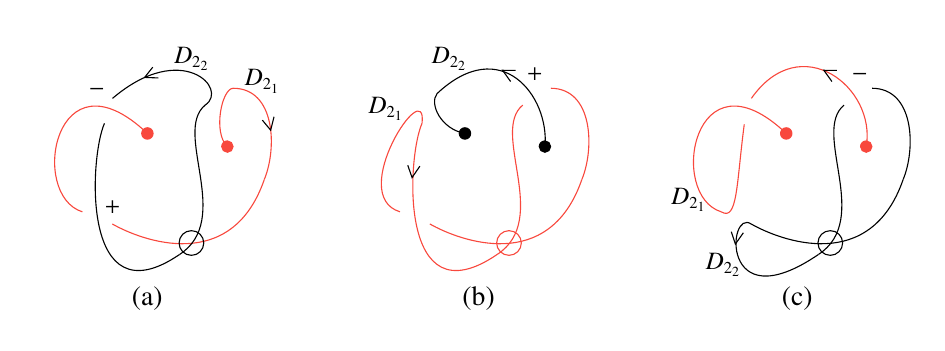
\begin{tikzpicture}[x=0.75pt,y=0.75pt,yscale=-0.9,xscale=0.9]		
					\draw    (85.96,656.6) .. controls (123.04,625.01) and (148.54,651.51) .. (135.58,660.18) ;
					\draw [color={rgb, 255:red, 248; green, 72; blue, 61 }  ,draw opacity=1 ]   (69.84,717.33) .. controls (40.84,708.33) and (55.21,628.44) .. (104.63,675.37) ;
					\draw [color={rgb, 255:red, 248; green, 72; blue, 61 }  ,draw opacity=1 ]   (85.84,723.83) .. controls (101.78,732.89) and (149.69,750.77) .. (167.22,700.01) ;
					\draw [color={rgb, 255:red, 248; green, 72; blue, 61 }  ,draw opacity=1 ]   (150.59,651.18) .. controls (173.32,651.28) and (174.02,683.64) .. (167.22,700.01) ;
					\draw    (135.58,660.18) .. controls (118.01,674.65) and (150.84,721.33) .. (121.86,740.16) ;
					\draw    (81.66,669.96) .. controls (73.6,687.95) and (68.84,776.33) .. (121.86,740.16) ; 
					\draw  [color={rgb, 255:red, 248; green, 72; blue, 61 }  ,draw opacity=1 ][fill={rgb, 255:red, 248; green, 72; blue, 61 }  ,fill opacity=1 ] (101.59,675.37) .. controls (101.59,673.69) and (102.95,672.33) .. (104.63,672.33) .. controls (106.31,672.33) and (107.67,673.69) .. (107.67,675.37) .. controls (107.67,677.05) and (106.31,678.41) .. (104.63,678.41) .. controls (102.95,678.41) and (101.59,677.05) .. (101.59,675.37) -- cycle ;
					\draw  [color={rgb, 255:red, 248; green, 72; blue, 61 }  ,draw opacity=1 ][fill={rgb, 255:red, 248; green, 72; blue, 61 }  ,fill opacity=1 ] (144.42,682.41) .. controls (144.42,680.73) and (145.78,679.37) .. (147.46,679.37) .. controls (149.13,679.37) and (150.49,680.73) .. (150.49,682.41) .. controls (150.49,684.08) and (149.13,685.44) .. (147.46,685.44) .. controls (145.78,685.44) and (144.42,684.08) .. (144.42,682.41) -- cycle ;
					\draw   (121.6,734.02) .. controls (121.6,730.37) and (124.56,727.41) .. (128.21,727.41) .. controls (131.85,727.41) and (134.81,730.37) .. (134.81,734.02) .. controls (134.81,737.66) and (131.85,740.62) .. (128.21,740.62) .. controls (124.56,740.62) and (121.6,737.66) .. (121.6,734.02) -- cycle ;
					\draw   (110.55,645.66) -- (103.16,645.37) -- (107.49,639.92) ;
					\draw    (259.69,654.04) .. controls (293.91,621.93) and (319.91,655.27) .. (317.46,682.41) ;
					\draw [color={rgb, 255:red, 248; green, 72; blue, 61 }  ,draw opacity=1 ]   (239.84,717.33) .. controls (210.84,708.33) and (254.57,642.6) .. (251.66,669.96) ;
					\draw [color={rgb, 255:red, 248; green, 72; blue, 61 }  ,draw opacity=1 ]   (255.84,723.83) .. controls (271.78,732.89) and (319.69,750.77) .. (337.22,700.01) ;
					\draw [color={rgb, 255:red, 248; green, 72; blue, 61 }  ,draw opacity=1 ]   (320.59,651.18) .. controls (343.32,651.28) and (344.02,683.64) .. (337.22,700.01) ;
					\draw [color={rgb, 255:red, 248; green, 72; blue, 61 }  ,draw opacity=1 ]   (305.58,660.18) .. controls (288.01,674.65) and (320.84,721.33) .. (291.86,740.16) ;
					\draw [color={rgb, 255:red, 248; green, 72; blue, 61 }  ,draw opacity=1 ]   (251.66,669.96) .. controls (243.6,687.95) and (238.84,776.33) .. (291.86,740.16) ;
					\draw  [fill={rgb, 255:red, 0; green, 0; blue, 0 }  ,fill opacity=1 ] (271.59,675.37) .. controls (271.59,673.69) and (272.95,672.33) .. (274.63,672.33) .. controls (276.31,672.33) and (277.67,673.69) .. (277.67,675.37) .. controls (277.67,677.05) and (276.31,678.41) .. (274.63,678.41) .. controls (272.95,678.41) and (271.59,677.05) .. (271.59,675.37) -- cycle ;
					\draw  [fill={rgb, 255:red, 0; green, 0; blue, 0 }  ,fill opacity=1 ] (314.42,682.41) .. controls (314.42,680.73) and (315.78,679.37) .. (317.46,679.37) .. controls (319.13,679.37) and (320.49,680.73) .. (320.49,682.41) .. controls (320.49,684.08) and (319.13,685.44) .. (317.46,685.44) .. controls (315.78,685.44) and (314.42,684.08) .. (314.42,682.41) -- cycle ;
					\draw  [color={rgb, 255:red, 248; green, 72; blue, 61 }  ,draw opacity=1 ] (291.6,734.02) .. controls (291.6,730.37) and (294.56,727.41) .. (298.21,727.41) .. controls (301.85,727.41) and (304.81,730.37) .. (304.81,734.02) .. controls (304.81,737.66) and (301.85,740.62) .. (298.21,740.62) .. controls (294.56,740.62) and (291.6,737.66) .. (291.6,734.02) -- cycle ;
					\draw   (299.08,647.57) -- (294.77,641.56) -- (301.73,641.64) ;
					\draw [color={rgb, 255:red, 248; green, 72; blue, 61 }  ,draw opacity=1 ]   (427.96,656.6) .. controls (454.32,619.05) and (494.95,650.73) .. (489.46,682.41) ;
					\draw [color={rgb, 255:red, 248; green, 72; blue, 61 }  ,draw opacity=1 ]   (411.84,717.33) .. controls (382.84,708.33) and (397.21,628.44) .. (446.63,675.37) ;
					\draw    (427.84,723.83) .. controls (443.78,732.89) and (491.69,750.77) .. (509.22,700.01) ;
					\draw    (492.59,651.18) .. controls (515.32,651.28) and (516.02,683.64) .. (509.22,700.01) ;
					\draw    (477.58,660.18) .. controls (460.01,674.65) and (492.84,721.33) .. (463.86,740.16) ;
					\draw    (427.84,723.83) .. controls (415.27,715.27) and (410.84,776.33) .. (463.86,740.16) ;
					\draw  [color={rgb, 255:red, 248; green, 72; blue, 61 }  ,draw opacity=1 ][fill={rgb, 255:red, 248; green, 72; blue, 61 }  ,fill opacity=1 ] (443.59,675.37) .. controls (443.59,673.69) and (444.95,672.33) .. (446.63,672.33) .. controls (448.31,672.33) and (449.67,673.69) .. (449.67,675.37) .. controls (449.67,677.05) and (448.31,678.41) .. (446.63,678.41) .. controls (444.95,678.41) and (443.59,677.05) .. (443.59,675.37) -- cycle ;
					\draw  [color={rgb, 255:red, 248; green, 72; blue, 61 }  ,draw opacity=1 ][fill={rgb, 255:red, 248; green, 72; blue, 61 }  ,fill opacity=1 ] (486.42,682.41) .. controls (486.42,680.73) and (487.78,679.37) .. (489.46,679.37) .. controls (491.13,679.37) and (492.49,680.73) .. (492.49,682.41) .. controls (492.49,684.08) and (491.13,685.44) .. (489.46,685.44) .. controls (487.78,685.44) and (486.42,684.08) .. (486.42,682.41) -- cycle ;
					\draw   (463.6,734.02) .. controls (463.6,730.37) and (466.56,727.41) .. (470.21,727.41) .. controls (473.85,727.41) and (476.81,730.37) .. (476.81,734.02) .. controls (476.81,737.66) and (473.85,740.62) .. (470.21,740.62) .. controls (466.56,740.62) and (463.6,737.66) .. (463.6,734.02) -- cycle ;
					\draw   (471.08,647.57) -- (466.77,641.56) -- (473.73,641.64) ;
					\draw [color={rgb, 255:red, 248; green, 72; blue, 61 }  ,draw opacity=1 ]   (150.59,651.18) .. controls (144.47,651.16) and (139.54,675.01) .. (147.46,682.41) ;
					\draw   (172.43,666.45) -- (170.61,673.61) -- (166.18,668.25) ;
					\draw    (259.69,654.04) .. controls (255.39,659.4) and (261.69,673.04) .. (274.63,675.37) ;
					\draw   (250.5,692.89) -- (246.32,698.98) -- (244.02,692.41) ;
					\draw [color={rgb, 255:red, 248; green, 72; blue, 61 }  ,draw opacity=1 ]   (411.84,717.33) .. controls (420.6,722.6) and (419.93,702.6) .. (424.15,670.51) ;
					\draw   (423.68,728.54) -- (419.41,734.57) -- (417.2,727.97) ;
					\draw (94.9,755.94) node [anchor=north west][inner sep=0.75pt]    {(a)};
					\draw (271.9,755.9) node [anchor=north west][inner sep=0.75pt]    {(b)};
					\draw (442.9,755.94) node [anchor=north west][inner sep=0.75pt]    {(c)};
					\draw (155.03,639.84) node [anchor=north west][inner sep=0.75pt]  [font=\small]  {$D_{2_{1}}$};
					\draw (117.27,627.84) node [anchor=north west][inner sep=0.75pt]  [font=\small]  {$D_{2_{2}}$};
					\draw (221.37,654.51) node [anchor=north west][inner sep=0.75pt]  [font=\small]  {$D_{2_{1}}$};
					\draw (255.18,627.84) node [anchor=north west][inner sep=0.75pt]  [font=\small]  {$D_{2_{2}}$};
					\draw (383.37,703.17) node [anchor=north west][inner sep=0.75pt]  [font=\small]  {$D_{2_{1}}$};
					\draw (401.85,738.17) node [anchor=north west][inner sep=0.75pt]  [font=\small]  {$D_{2_{2}}$};
					\draw (80.32,710.18) node [anchor=north west][inner sep=0.75pt]  [font=\small]  {$+$};
					\draw (71.84,646.58) node [anchor=north west][inner sep=0.75pt]  [font=\small]  {$-$};
					\draw (306.34,639.08) node [anchor=north west][inner sep=0.75pt]  [font=\small]  {$+$};
					\draw (480.34,638.58) node [anchor=north west][inner sep=0.75pt]  [font=\small]  {$-$};
				\end{tikzpicture}
				\caption{(a)--(c): Diagrams obtained by orientation-preserving smoothing at classical crossings $c_1$, $c_2$, and $c_3$ in $D_2$.} \label{fig605}
			\end{center}
		\end{figure}
		From Fig.~\ref{fig605}, we obtain $I(c_1)=2$, $I(c_2)=I(c_3)=1$, thus $c_2,c_3\in O(D_1)$ and $c_1\in E(D_1)$. Then we have $J(K_1)=J(K_2)=-2$.
		
		
		\begin{figure}[!ht]
			\begin{center}
				\tikzset{every picture/.style={line width=1.pt}}  
				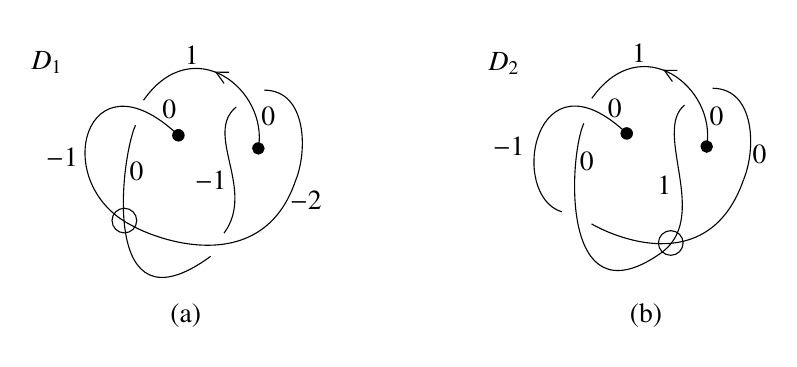
\begin{tikzpicture}[x=0.75pt,y=0.75pt,yscale=-0.9,xscale=0.9]		
					\draw    (130.96,275.54) .. controls (157.32,237.99) and (197.95,269.67) .. (192.46,301.35) ;
					\draw    (124.37,342.41) .. controls (79.55,319.4) and (100.21,247.38) .. (149.63,294.31) ;
					\draw    (124.37,342.41) .. controls (140.32,351.47) and (194.69,369.71) .. (212.22,318.95) ;
					\draw    (195.59,270.12) .. controls (218.32,270.22) and (219.02,302.58) .. (212.22,318.95) ;
					\draw    (180.58,279.12) .. controls (163.01,293.59) and (191.27,323.23) .. (174.06,346.7) ;
					\draw    (126.66,288.9) .. controls (118.6,306.89) and (107.39,402.8) .. (166.86,359.1) ; 
					\draw  [fill={rgb, 255:red, 0; green, 0; blue, 0 }  ,fill opacity=1 ] (146.59,294.31) .. controls (146.59,292.63) and (147.95,291.27) .. (149.63,291.27) .. controls (151.31,291.27) and (152.67,292.63) .. (152.67,294.31) .. controls (152.67,295.99) and (151.31,297.35) .. (149.63,297.35) .. controls (147.95,297.35) and (146.59,295.99) .. (146.59,294.31) -- cycle ;
					\draw  [fill={rgb, 255:red, 0; green, 0; blue, 0 }  ,fill opacity=1 ] (189.42,301.35) .. controls (189.42,299.67) and (190.78,298.31) .. (192.46,298.31) .. controls (194.13,298.31) and (195.49,299.67) .. (195.49,301.35) .. controls (195.49,303.02) and (194.13,304.38) .. (192.46,304.38) .. controls (190.78,304.38) and (189.42,303.02) .. (189.42,301.35) -- cycle ;
					\draw   (114.1,339.96) .. controls (114.1,336.31) and (117.06,333.35) .. (120.71,333.35) .. controls (124.35,333.35) and (127.31,336.31) .. (127.31,339.96) .. controls (127.31,343.6) and (124.35,346.56) .. (120.71,346.56) .. controls (117.06,346.56) and (114.1,343.6) .. (114.1,339.96) -- cycle ;
					\draw   (174.08,266.51) -- (169.77,260.5) -- (176.73,260.58) ;
					\draw    (370.96,274.54) .. controls (397.32,236.99) and (437.95,268.67) .. (432.46,300.35) ;
					\draw    (354.84,335.27) .. controls (325.84,326.27) and (340.21,246.38) .. (389.63,293.31) ;
					\draw    (370.84,341.77) .. controls (386.78,350.83) and (434.69,368.71) .. (452.22,317.95) ;
					\draw    (435.59,269.12) .. controls (458.32,269.22) and (459.02,301.58) .. (452.22,317.95) ;
					\draw    (420.58,278.12) .. controls (403.01,292.59) and (435.84,339.27) .. (406.86,358.1) ; 
					\draw    (366.66,287.9) .. controls (358.6,305.89) and (353.84,394.27) .. (406.86,358.1) ;
					\draw  [fill={rgb, 255:red, 0; green, 0; blue, 0 }  ,fill opacity=1 ] (386.59,293.31) .. controls (386.59,291.63) and (387.95,290.27) .. (389.63,290.27) .. controls (391.31,290.27) and (392.67,291.63) .. (392.67,293.31) .. controls (392.67,294.99) and (391.31,296.35) .. (389.63,296.35) .. controls (387.95,296.35) and (386.59,294.99) .. (386.59,293.31) -- cycle ;
					\draw  [fill={rgb, 255:red, 0; green, 0; blue, 0 }  ,fill opacity=1 ] (429.42,300.35) .. controls (429.42,298.67) and (430.78,297.31) .. (432.46,297.31) .. controls (434.13,297.31) and (435.49,298.67) .. (435.49,300.35) .. controls (435.49,302.02) and (434.13,303.38) .. (432.46,303.38) .. controls (430.78,303.38) and (429.42,302.02) .. (429.42,300.35) -- cycle ;
					\draw   (406.6,351.96) .. controls (406.6,348.31) and (409.56,345.35) .. (413.21,345.35) .. controls (416.85,345.35) and (419.81,348.31) .. (419.81,351.96) .. controls (419.81,355.6) and (416.85,358.56) .. (413.21,358.56) .. controls (409.56,358.56) and (406.6,355.6) .. (406.6,351.96) -- cycle ;
					\draw   (414.08,265.51) -- (409.77,259.5) -- (416.73,259.58) ;
					\draw (69.24,247.94) node [anchor=north west][inner sep=0.75pt]    {$D_{1}$};
					\draw (313.9,248.44) node [anchor=north west][inner sep=0.75pt]    {$D_{2}$};
					\draw (143.9,382.94) node [anchor=north west][inner sep=0.75pt]    {(a)};
					\draw (389.9,382.94) node [anchor=north west][inner sep=0.75pt]    {(b)};
					\draw (192.66,277.54) node [anchor=north west][inner sep=0.75pt]    {$0$};
					\draw (157.16,312.04) node [anchor=north west][inner sep=0.75pt]    {$-1$};
					\draw (151.66,245.04) node [anchor=north west][inner sep=0.75pt]    {$1$};
					\draw (432.66,277.94) node [anchor=north west][inner sep=0.75pt]    {$0$};
					\draw (77.66,299.44) node [anchor=north west][inner sep=0.75pt]    {$-1$};
					\draw (122.16,307.44) node [anchor=north west][inner sep=0.75pt]    {$0$};
					\draw (208.16,322.94) node [anchor=north west][inner sep=0.75pt]    {$-2$};
					\draw (391.16,243.94) node [anchor=north west][inner sep=0.75pt]    {$1$};
					\draw (139.66,273.94) node [anchor=north west][inner sep=0.75pt]    {$0$};
					\draw (316.66,293.94) node [anchor=north west][inner sep=0.75pt]    {$-1$};
					\draw (404.66,314.44) node [anchor=north west][inner sep=0.75pt]    {$1$};
					\draw (363.16,301.94) node [anchor=north west][inner sep=0.75pt]    {$0$};
					\draw (455.66,297.94) node [anchor=north west][inner sep=0.75pt]    {$0$};
					\draw (378.16,273.44) node [anchor=north west][inner sep=0.75pt]    {$0$};
				\end{tikzpicture}
				\caption{Integer labeling for $D_1$ and $D_2$, respectively.} \label{fig603}
			\end{center}
		\end{figure}     
		Now we compute $\mathbf{P}_{K_1}(x,y)$ and $\mathbf{P}_{K_2}(x,y)$.  Based on Fig.~\ref{fig603}(a), we have 
		$$
		W_{D_1}(c_1)=-(-1-1)=2, \quad W_{D_1}(c_2)=-(1-0)=-1, \quad
		W_{D_1}(c_3)=-(0-(-1))=-1.
		$$  
		From Fig.~\ref{fig604} we get $i(c_1)=-2$, $i(c_2)=1$, $i(c_3)=1$. Therefore, 
		$$
		\mathbf{P}_{K_1}(x,y)=-(-2)x^2-y^{-1}-y^{-1}=2x^2-2y^{-1}.
		$$ 
		
		Based on Fig.~\ref{fig603}(b), we have 
		$$
		W_{D_2}(c_1)=-(1-1)=0, \quad W_{D_2}(c_2)=-(1-0)=-1, \quad
		W_{D_2}(c_3)=-(0-1)=1.
		$$ 
		From Fig.~\ref{fig605} we get $i(c_1)=0$, $i(c_2)=1$, $i(c_3)=-1$. Therefore, 
		$$
		\mathbf{P}_{K_2}(x,y)=-0-y^{-1}-(-1)y=y-y^{-1}.
		$$ 
		From the foregoing considerations, we conclude that $\mathbf{P}_{K_1}(x,y)\neq \mathbf{P}_{K_2}(x,y)$. Hence, $K_1$ and $K_2$ are distinct virtual knotoids.    
	}
\end{example}

\subsection{$\mathbf{P}_K(x,y)$ and the affine index polynomial} \label{subsection3.1}

For an oriented virtual knotoid $K$, let $AI_K(t)$ be the affine index polynomial of $K$ defined in~\cite{GK}. Recall that for a virtual or classical knotoid diagram $K$, its affine index polynomial is defined by $AI_K(t)=\sum_{c}\operatorname{sgn}(c)\bigl(t^{w_K(c)}-1\bigr)$. We show that $\mathbf{P}_K(x,y)$ is equivalent to $AI_K(t)$.


We begin with the following lemma, which will be needed in the proof of Theorem~\ref{thm2}.	

\begin{lemma}\label{lm2}
	Let $D$ be an oriented virtual knotoid diagram and let $c$ be a classical crossing of $D$. Then the intersection index $i(c)$ has the same parity as the crossing $c$.
\end{lemma}

\begin{proof}
	Suppose that the orientation-preserving smoothing at $c$ produces the ordered two-component virtual knotoid diagram $D_1\cup D_2$.
	
	By definition,
	$ i(c)=\sum_{e\in D_1\cap D_2}\operatorname{ind}(e)$,	
	where $\operatorname{ind}(e)=\pm1$. Hence,
	$$
	i(c)\equiv
	\sum_{e\in D_1\cap D_2}1=I(c)\pmod2,
	$$
	where $I(c)$ denotes the number of classical crossings between the two components $D_1$ and $D_2$. Since the parity of the crossing $c$ is defined by the parity of $I(c)$, see subsection~\ref{subsection2.2}, it follows that $i(c)$ and $c$ have the same parity.
\end{proof}

Let $D$ be an oriented virtual knotoid diagram and let $c$ be a classical crossing of $D$. Consider the diagram obtained by applying the orientation-preserving smoothing, also known as  $1$-smoothing, at the crossing $c$. This operation produces a two-component diagram, denoted by $D_1 \cup D_2$. The following relation between the $i(c)$ and the $W_D(c)$ will be useful, where $i(c)$ denotes the intersection index of $c$ and $W_D(c)$ denotes the weight of $c$.

We note that $i(c) = -W(D_1\cup D_2)$, where $W(D_1\cup D_2)$ denotes the wiggle number defined in~\cite{FK}. From the proof of Theorem 7 in~\cite{FK}, we have $W(D_1\cup D_2)=W_D(c)$, which yields the following conclusion.

\begin{lemma}
	$i(c)=-W_D(c)$. \label{lm1}
\end{lemma}

Combined with Lemma~\ref{lm2}, we have

\begin{corollary} \label{cor:weight-parity}
	Let $D$ be an oriented virtual knotoid diagram and let $c$ be a classical crossing of $D$.	Then $W_D(c)$ and $c$ have the same parity.
\end{corollary}

We now turn to a discussion of the relation between $\mathbf{P}_K(x,y)$ and $AI_K(t)$.

\begin{definition}
	Let $\mathbf{Q}^1$ and $\mathbf{Q}^2$ be two invariants of virtual knotoid. We say that $\mathbf{Q}^1$ and $\mathbf{Q}^2$ are equivalent if $$\mathbf{Q}^1_{K_1}=\mathbf{Q}^1_{K_2} \iff \mathbf{Q}^2_{K_1}=\mathbf{Q}^2_{K_2},$$ for any virtual knotoids $K_1$ and $K_2$.
\end{definition}


\begin{theorem}\label{thm2} 
	The two-variable parity polynomial $\mathbf{P}_D(x,y)$ and the affine index polynomial $AI_K(t)$ are equivalent invariants, that is, for any two oriented virtual knotoids $K_1$ and $K_2$,
	$$
	AI_{K_1}(t)=AI_{K_2}(t)
	\iff
	\mathbf P_{K_1}(x,y)=
	\mathbf P_{K_2}(x,y).
	$$
\end{theorem}

\begin{proof}
	For every oriented virtual knotoid diagram $D$, write
	\[
	AI_D(t)=
	\sum_{m\neq0}
	a_m(D)(t^m-1),
	\]
	where
	$
	a_m(D)=
	\sum_{\substack{c\in C(D)\\W_D(c)=m}}
	\operatorname{sgn}(c).
	$
	Let $V$ be the free abelian group with basis
	$\{\,t^m-1\mid m\neq0\,\}$, there exists a unique
	$\mathbb Z$-linear map
	$
	\Phi:V\longrightarrow
	\mathbb Z[x^{\pm1},y^{\pm1}]
	$
	defined by
	\[
	\Phi(t^m-1)=
	\begin{cases}
		-mx^m,&m\text{ even},\\[1ex]
		-my^m,&m\text{ odd}.
	\end{cases}
	\]
	
	By Lemma~\ref{lm1} and Corollary~\ref{cor:weight-parity}, we have
	$i(c)=-W_D(c)$, and the weight $W_D(c)$ has the same parity as the crossing $c$.
	Hence,
	\begin{equation} \label{equ6}
		\mathbf P_D(x,y)
		=
		\Phi(AI_D(t)).	
	\end{equation}
	Suppose first that
	$
	AI_{K_1}(t)=AI_{K_2}(t).
	$
	Applying $\Phi$ to both sides gives
	\[
	\mathbf P_{K_1}(x,y)
	=
	\Phi(AI_{K_1}(t))
	=
	\Phi(AI_{K_2}(t))
	=
	\mathbf P_{K_2}(x,y).
	\]
	Conversely, suppose that
	$
	\mathbf P_{K_1}(x,y)
	=
	\mathbf P_{K_2}(x,y).
	$
	Then
	$
	\Phi\!\left(
	AI_{K_1}(t)-AI_{K_2}(t)
	\right)=0.
	$
	Since
	\[
	\Phi\!\left(
	\sum_{m\neq0}a_m(t^m-1)
	\right)
	=
	-\sum_{\substack{m\neq0\\m\text{ even}}}
	ma_mx^m
	-
	\sum_{\substack{m\text{ odd}}}
	ma_my^m,
	\]
	and the monomials
	$
	\{x^m\mid m\neq0,\;m\text{ even}\}
	\cup
	\{y^m\mid m\neq0,\;m\text{ odd}\}
	$
	are linearly independent over $\mathbb Z$, it follows that
	$ma_m=0$ for every $m\neq0$, and hence $a_m=0$ for all $m\neq0$.
	Therefore,
	$
	AI_{K_1}(t)-AI_{K_2}(t)=0,
	$
	that is,
	$
	AI_{K_1}(t)=AI_{K_2}(t).
	$
	
	This completes the proof.	
\end{proof}


Although the two-variable parity polynomial $\mathbf{P}_K(x,y)$ is equivalent to the affine index polynomial $AI_K(t)$, under the specialization $x=y=t$, the two polynomials are, in general, not equal. The following example illustrates this.


\begin{example} \label{exp3}
	{\rm
		Let $K_1$ and $K_2$  be oriented virtual knotoids with diagrams $D_1$ and $D_2$ presented in Fig.~\ref{fig514}. 
		\begin{figure}[!ht]
			\begin{center}
				\tikzset{every picture/.style={line width=1.pt}}  
				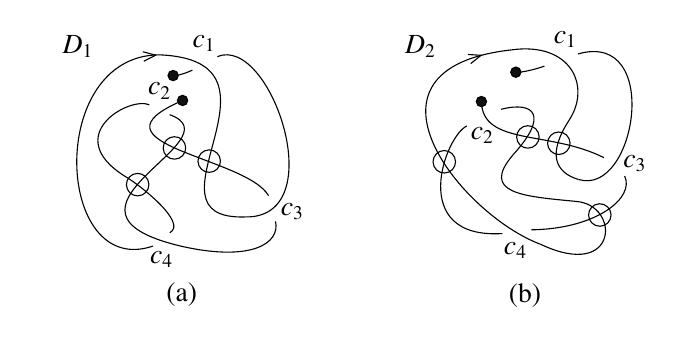
\begin{tikzpicture}[x=0.75pt,y=0.75pt,yscale=-1,xscale=1]	
					\draw    (115.14,104.96) .. controls (68,121.01) and (63.39,13.38) .. (118.06,12.81) ;
					\draw    (118.06,12.81) .. controls (187.45,15.54) and (105.67,92.64) .. (159.61,90.92) ;
					\draw    (129.41,34.81) .. controls (80.38,55.91) and (159.89,61.87) .. (170.84,80.67) ;
					\draw    (159.61,90.92) .. controls (201.79,91.67) and (171.87,3.02) .. (146.16,13.67) ;
					\draw    (123.15,41.64) .. controls (157.08,53.83) and (55.04,87.97) .. (129.54,105.2) ; 
					\draw    (113.36,36.87) .. controls (103.64,32.72) and (70.83,51.6) .. (101.2,71.06) ; 
					\draw    (101.2,71.06) .. controls (108.49,75.21) and (132.14,93.76) .. (123.23,98.55) ; 
					\draw    (129.54,105.2) .. controls (162.75,112.54) and (176.56,103.59) .. (174.18,93.04) ;
					\draw   (130.9,57.58) .. controls (130.96,60.57) and (128.57,63.04) .. (125.58,63.09) .. controls (122.59,63.15) and (120.12,60.76) .. (120.07,57.77) .. controls (120.02,54.78) and (122.4,52.31) .. (125.39,52.26) .. controls (128.38,52.21) and (130.85,54.59) .. (130.9,57.58) -- cycle ;
					\draw   (113.18,75.26) .. controls (113.23,78.25) and (110.85,80.72) .. (107.85,80.77) .. controls (104.86,80.82) and (102.39,78.44) .. (102.34,75.45) .. controls (102.29,72.46) and (104.67,69.99) .. (107.67,69.94) .. controls (110.66,69.88) and (113.13,72.27) .. (113.18,75.26) -- cycle ; 
					\draw   (147.65,63.93) .. controls (147.71,66.92) and (145.32,69.39) .. (142.33,69.44) .. controls (139.34,69.49) and (136.87,67.11) .. (136.82,64.12) .. controls (136.77,61.12) and (139.15,58.66) .. (142.14,58.6) .. controls (145.13,58.55) and (147.6,60.93) .. (147.65,63.93) -- cycle ;
					\draw    (124.86,22.8) .. controls (126.77,23.15) and (132.11,21.19) .. (134.11,20.18) ;
					\draw  [fill={rgb, 255:red, 17; green, 16; blue, 16 }  ,fill opacity=1 ] (127.34,22.77) .. controls (127.32,21.41) and (126.2,20.31) .. (124.84,20.32) .. controls (123.47,20.34) and (122.38,21.46) .. (122.39,22.83) .. controls (122.41,24.2) and (123.53,25.3) .. (124.89,25.28) .. controls (126.26,25.26) and (127.35,24.14) .. (127.34,22.77) -- cycle ; 
					\draw  [fill={rgb, 255:red, 17; green, 16; blue, 16 }  ,fill opacity=1 ] (131.88,34.78) .. controls (131.86,33.41) and (130.75,32.31) .. (129.38,32.33) .. controls (128.02,32.34) and (126.92,33.46) .. (126.94,34.83) .. controls (126.95,36.2) and (128.07,37.3) .. (129.44,37.28) .. controls (130.8,37.27) and (131.89,36.15) .. (131.88,34.78) -- cycle ;
					\draw   (110.26,11.32) -- (116.43,12.98) -- (110.75,15.9) ;
					\draw    (301.98,104.13) .. controls (264.01,90.12) and (206.42,19.46) .. (287.98,10.42) ;
					\draw    (287.98,10.42) .. controls (316.61,6.52) and (326.3,27.93) .. (315.71,44.18) .. controls (305.13,60.44) and (308.7,69.46) .. (320.19,72.88) ;
					\draw    (273.38,35.33) .. controls (273.93,56.8) and (305.9,49.01) .. (332.43,62.37) ;
					\draw    (320.19,72.88) .. controls (347.88,81.3) and (360.67,0.64) .. (319.89,12.41) ; 
					\draw    (282.87,39.06) .. controls (298.99,34.96) and (305.86,42.04) .. (288.84,60.74) ;
					\draw    (266.42,47.05) .. controls (255.87,51.85) and (237.49,101.74) .. (283.47,98.92) ; 
					\draw    (301.98,104.13) .. controls (339.6,121.87) and (340.49,85.08) .. (319,83.44) ; 
					\draw    (288.84,60.74) .. controls (272.42,79.7) and (293.62,80.98) .. (319,83.44) ;
					\draw    (289.96,21.18) .. controls (292.8,21.57) and (300.75,19.38) .. (303.74,18.25) ;
					\draw  [fill={rgb, 255:red, 17; green, 16; blue, 16 }  ,fill opacity=1 ] (292.43,21.15) .. controls (292.41,19.78) and (291.3,18.69) .. (289.93,18.7) .. controls (288.57,18.72) and (287.47,19.84) .. (287.49,21.21) .. controls (287.5,22.58) and (288.62,23.68) .. (289.99,23.66) .. controls (291.35,23.64) and (292.44,22.52) .. (292.43,21.15) -- cycle ;
					\draw  [fill={rgb, 255:red, 17; green, 16; blue, 16 }  ,fill opacity=1 ] (275.85,35.3) .. controls (275.83,33.93) and (274.71,32.84) .. (273.35,32.85) .. controls (271.98,32.87) and (270.89,33.99) .. (270.9,35.36) .. controls (270.92,36.73) and (272.04,37.82) .. (273.4,37.81) .. controls (274.77,37.79) and (275.86,36.67) .. (275.85,35.3) -- cycle ;
					\draw   (266.85,12.65) -- (273.23,13.04) -- (268.25,17.04) ;
					\draw    (297.5,97.12) .. controls (329.74,96.61) and (347.34,81.21) .. (342.37,71.22) ;
					\draw   (260.91,64.25) .. controls (260.97,67.24) and (258.58,69.71) .. (255.59,69.76) .. controls (252.6,69.81) and (250.13,67.43) .. (250.08,64.44) .. controls (250.03,61.45) and (252.41,58.98) .. (255.4,58.93) .. controls (258.39,58.87) and (260.86,61.26) .. (260.91,64.25) -- cycle ;
					\draw   (316.09,55.32) .. controls (316.14,58.31) and (313.76,60.78) .. (310.77,60.83) .. controls (307.78,60.88) and (305.31,58.5) .. (305.26,55.51) .. controls (305.2,52.52) and (307.59,50.05) .. (310.58,50) .. controls (313.57,49.94) and (316.04,52.33) .. (316.09,55.32) -- cycle ; 
					\draw   (335.84,89.89) .. controls (335.89,92.88) and (333.51,95.35) .. (330.52,95.4) .. controls (327.53,95.46) and (325.06,93.07) .. (325.01,90.08) .. controls (324.95,87.09) and (327.34,84.62) .. (330.33,84.57) .. controls (333.32,84.52) and (335.79,86.9) .. (335.84,89.89) -- cycle ;
					\draw   (301.2,52.28) .. controls (301.25,55.27) and (298.87,57.74) .. (295.88,57.79) .. controls (292.88,57.84) and (290.42,55.46) .. (290.36,52.47) .. controls (290.31,49.48) and (292.7,47.01) .. (295.69,46.96) .. controls (298.68,46.9) and (301.15,49.29) .. (301.2,52.28) -- cycle ;
					\draw (120.33,121.67) node [anchor=north west][inner sep=0.75pt]    {(a)};
					\draw (285.33,121.67) node [anchor=north west][inner sep=0.75pt]    {(b)};
					\draw (70,2) node [anchor=north west][inner sep=0.75pt]    {$D_{1}$};
					\draw (235,2) node [anchor=north west][inner sep=0.75pt]    {$D_{2}$};
					\draw (133,2) node [anchor=north west][inner sep=0.75pt]    {$c_{1}$};
					\draw (111.5,25) node [anchor=north west][inner sep=0.75pt]    {$c_{2}$};
					\draw (175.5,83) node [anchor=north west][inner sep=0.75pt]    {$c_{3}$};
					\draw (112.5,106) node [anchor=north west][inner sep=0.75pt]    {$c_{4}$};
					\draw (307,0) node [anchor=north west][inner sep=0.75pt]    {$c_{1}$};
					\draw (267,46.5) node [anchor=north west][inner sep=0.75pt]    {$c_{2}$};
					\draw (340.5,60) node [anchor=north west][inner sep=0.75pt]    {$c_{3}$};
					\draw (283,102) node [anchor=north west][inner sep=0.75pt]    {$c_{4}$};	    
				\end{tikzpicture}
				\caption{Virtual knotoid diagrams $D_1$ and $D_2$.} \label{fig514}
			\end{center}
		\end{figure} 
		The diagram $D_1$ contains three virtual crossings and four classical crossings $c_1$, $c_2$, $c_3$ and $c_4$. One can see from Fig.~\ref{fig514}(a) that 
		$$
		\operatorname{sgn}(c_1)=\operatorname{sgn}(c_2)=\operatorname{sgn}(c_3)=-1, \quad \operatorname{sgn}(c_4)=1.
		$$ 
		\begin{figure}[!ht]
			\begin{center}
				\tikzset{every picture/.style={line width=1.0pt}}  
				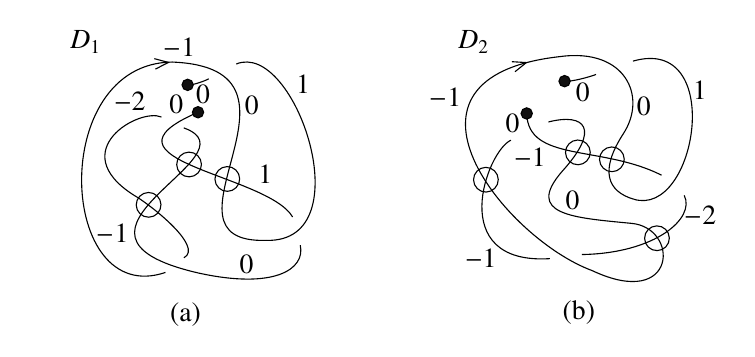
\begin{tikzpicture}[x=0.75pt,y=0.75pt,yscale=-1.1,xscale=1.1]
					\draw    (118.14,286.96) .. controls (71,303.01) and (66.39,195.38) .. (121.06,194.81) ;
					\draw    (121.06,194.81) .. controls (190.45,197.54) and (108.67,274.64) .. (162.61,272.92) ;
					\draw    (132.41,216.81) .. controls (83.38,237.91) and (162.89,243.87) .. (173.84,262.67) ;
					\draw    (162.61,272.92) .. controls (204.79,273.67) and (174.87,185.02) .. (149.16,195.67) ; 
					\draw    (126.15,223.64) .. controls (160.08,235.83) and (58.04,269.97) .. (132.54,287.2) ; 
					\draw    (116.36,218.87) .. controls (106.64,214.72) and (73.83,233.6) .. (104.2,253.06) ; 
					\draw    (104.2,253.06) .. controls (111.49,257.21) and (135.14,275.76) .. (126.23,280.55) ; 
					\draw    (132.54,287.2) .. controls (165.75,294.54) and (179.56,285.59) .. (177.18,275.04) ; 
					\draw   (133.9,239.58) .. controls (133.96,242.57) and (131.57,245.04) .. (128.58,245.09) .. controls (125.59,245.15) and (123.12,242.76) .. (123.07,239.77) .. controls (123.02,236.78) and (125.4,234.31) .. (128.39,234.26) .. controls (131.38,234.21) and (133.85,236.59) .. (133.9,239.58) -- cycle ; 
					\draw   (116.18,257.26) .. controls (116.23,260.25) and (113.85,262.72) .. (110.85,262.77) .. controls (107.86,262.82) and (105.39,260.44) .. (105.34,257.45) .. controls (105.29,254.46) and (107.67,251.99) .. (110.67,251.94) .. controls (113.66,251.88) and (116.13,254.27) .. (116.18,257.26) -- cycle ; 
					\draw   (150.65,245.93) .. controls (150.71,248.92) and (148.32,251.39) .. (145.33,251.44) .. controls (142.34,251.49) and (139.87,249.11) .. (139.82,246.12) .. controls (139.77,243.12) and (142.15,240.66) .. (145.14,240.6) .. controls (148.13,240.55) and (150.6,242.93) .. (150.65,245.93) -- cycle ;
					\draw    (127.86,204.8) .. controls (129.77,205.15) and (135.11,203.19) .. (137.11,202.18) ; 
					\draw  [fill={rgb, 255:red, 17; green, 16; blue, 16 }  ,fill opacity=1 ] (130.34,204.77) .. controls (130.32,203.41) and (129.2,202.31) .. (127.84,202.32) .. controls (126.47,202.34) and (125.38,203.46) .. (125.39,204.83) .. controls (125.41,206.2) and (126.53,207.3) .. (127.89,207.28) .. controls (129.26,207.26) and (130.35,206.14) .. (130.34,204.77) -- cycle ; 
					\draw  [fill={rgb, 255:red, 17; green, 16; blue, 16 }  ,fill opacity=1 ] (134.88,216.78) .. controls (134.86,215.41) and (133.75,214.31) .. (132.38,214.33) .. controls (131.02,214.34) and (129.92,215.46) .. (129.94,216.83) .. controls (129.95,218.2) and (131.07,219.3) .. (132.44,219.28) .. controls (133.8,219.27) and (134.89,218.15) .. (134.88,216.78) -- cycle ;
					\draw   (113.26,193.32) -- (119.43,194.98) -- (113.75,197.9) ;
					\draw    (304.98,286.13) .. controls (267.01,272.12) and (209.42,201.46) .. (290.98,192.42) ;
					\draw    (290.98,192.42) .. controls (319.61,188.52) and (329.3,209.93) .. (318.71,226.18) .. controls (308.13,242.44) and (311.7,251.46) .. (323.19,254.88) ; 
					\draw    (276.38,217.33) .. controls (276.93,238.8) and (308.9,231.01) .. (335.43,244.37) ;
					\draw    (323.19,254.88) .. controls (350.88,263.3) and (363.67,182.64) .. (322.89,194.41) ; 
					\draw    (285.87,221.06) .. controls (301.99,216.96) and (308.86,224.04) .. (291.84,242.74) ;
					\draw    (269.42,229.05) .. controls (258.87,233.85) and (240.49,283.74) .. (286.47,280.92) ; 
					\draw    (304.98,286.13) .. controls (342.6,303.87) and (343.49,267.08) .. (322,265.44) ; 
					\draw    (291.84,242.74) .. controls (275.42,261.7) and (296.62,262.98) .. (322,265.44) ;
					\draw    (292.96,203.18) .. controls (295.8,203.57) and (303.75,201.38) .. (306.74,200.25) ; 
					\draw  [fill={rgb, 255:red, 17; green, 16; blue, 16 }  ,fill opacity=1 ] (295.43,203.15) .. controls (295.41,201.78) and (294.3,200.69) .. (292.93,200.7) .. controls (291.57,200.72) and (290.47,201.84) .. (290.49,203.21) .. controls (290.5,204.58) and (291.62,205.68) .. (292.99,205.66) .. controls (294.35,205.64) and (295.44,204.52) .. (295.43,203.15) -- cycle ; 
					\draw  [fill={rgb, 255:red, 17; green, 16; blue, 16 }  ,fill opacity=1 ] (278.85,217.3) .. controls (278.83,215.93) and (277.71,214.84) .. (276.35,214.85) .. controls (274.98,214.87) and (273.89,215.99) .. (273.9,217.36) .. controls (273.92,218.73) and (275.04,219.82) .. (276.4,219.81) .. controls (277.77,219.79) and (278.86,218.67) .. (278.85,217.3) -- cycle ;
					\draw   (269.85,194.65) -- (276.23,195.04) -- (271.25,199.04) ;
					\draw    (300.5,279.12) .. controls (332.74,278.61) and (350.34,263.21) .. (345.37,253.22) ; 
					\draw   (263.91,246.25) .. controls (263.97,249.24) and (261.58,251.71) .. (258.59,251.76) .. controls (255.6,251.81) and (253.13,249.43) .. (253.08,246.44) .. controls (253.03,243.45) and (255.41,240.98) .. (258.4,240.93) .. controls (261.39,240.87) and (263.86,243.26) .. (263.91,246.25) -- cycle ; 
					\draw   (319.09,237.32) .. controls (319.14,240.31) and (316.76,242.78) .. (313.77,242.83) .. controls (310.78,242.88) and (308.31,240.5) .. (308.26,237.51) .. controls (308.2,234.52) and (310.59,232.05) .. (313.58,232) .. controls (316.57,231.94) and (319.04,234.33) .. (319.09,237.32) -- cycle ;
					\draw   (338.84,271.89) .. controls (338.89,274.88) and (336.51,277.35) .. (333.52,277.4) .. controls (330.53,277.46) and (328.06,275.07) .. (328.01,272.08) .. controls (327.95,269.09) and (330.34,266.62) .. (333.33,266.57) .. controls (336.32,266.52) and (338.79,268.9) .. (338.84,271.89) -- cycle ;
					\draw   (304.2,234.28) .. controls (304.25,237.27) and (301.87,239.74) .. (298.88,239.79) .. controls (295.88,239.84) and (293.42,237.46) .. (293.36,234.47) .. controls (293.31,231.48) and (295.7,229.01) .. (298.69,228.96) .. controls (301.68,228.9) and (304.15,231.29) .. (304.2,234.28) -- cycle ;
					\draw (118.73,208) node [anchor=north west][inner sep=0.75pt]    {$0$};
					\draw (174.23,199.39) node [anchor=north west][inner sep=0.75pt]    {$1$};
					\draw (116.23,183.14) node [anchor=north west][inner sep=0.75pt]    {$-1$};
					\draw (94.48,206.89) node [anchor=north west][inner sep=0.75pt]    {$-2$};
					\draw (323.48,209) node [anchor=north west][inner sep=0.75pt]    {$0$};
					\draw (292.23,250) node [anchor=north west][inner sep=0.75pt]    {$0$};
					\draw (296.73,203) node [anchor=north west][inner sep=0.75pt]    {$0$};
					\draw (347.98,201.89) node [anchor=north west][inner sep=0.75pt]    {$1$};
					\draw (265.98,216.25) node [anchor=north west][inner sep=0.75pt]    {$0$};
					\draw (232.73,204.89) node [anchor=north west][inner sep=0.75pt]    {$-1$};
					\draw (151.73,208.5) node [anchor=north west][inner sep=0.75pt]    {$0$};
					\draw (269.73,231.14) node [anchor=north west][inner sep=0.75pt]    {$-1$};
					\draw (149.48,278.25) node [anchor=north west][inner sep=0.75pt]    {$0$};
					\draw (248.23,275.64) node [anchor=north west][inner sep=0.75pt]    {$-1$};
					\draw (344.48,256.64) node [anchor=north west][inner sep=0.75pt]    {$-2$};
					\draw (130.48,203.5) node [anchor=north west][inner sep=0.75pt]    {$0$};
					\draw (157.73,238.89) node [anchor=north west][inner sep=0.75pt]    {$1$};
					\draw (86.98,264.39) node [anchor=north west][inner sep=0.75pt]    {$-1$};
					\draw (119,299.13) node [anchor=north west][inner sep=0.75pt]    {(a)};
					\draw (291,298.28) node [anchor=north west][inner sep=0.75pt]    {(b)};
					\draw (75,180) node [anchor=north west][inner sep=0.75pt]    {$D_1$};
					\draw (245,180) node [anchor=north west][inner sep=0.75pt]    {$D_2$};
				\end{tikzpicture}
				\caption{Integer labeling for $D_1$ and $D_2$, respectively.} \label{fig515}
			\end{center}
		\end{figure} 
		Based on Fig.~\ref{fig515}(a), we have 
		$$
		\begin{gathered}
			W_{D_1}(c_1)=-(1-0)=-1, \quad W_{D_1}(c_2)=-(-1-1)=2, \cr 
			W_{D_1}(c_3)=-(1-1)=0, \quad W_{D_1}(c_4)=0-(-1)=1.
		\end{gathered}
		$$
		The diagram $D_2$ contains four virtual crossings and four classical crossings $c_1$, $c_2$, $c_3$ and $c_4$. One can see from Fig.~\ref{fig514}(b) that 
		$$
		\operatorname{sgn}(c_1)=\operatorname{sgn}(c_3)=-1, \quad \operatorname{sgn}(c_2)=\operatorname{sgn}(c_4)=1.
		$$ 
		Based on Fig.~\ref{fig515}(b), we have 
		$$
		\begin{gathered} 
			W_{D_2}(c_1)=-(1-0)=-1, \quad W_{D_2}(c_2)=0-0=0, \cr 
			W_{D_2}(c_3)=-(-1-1)=2, \quad W_{D_2}(c_4)=0-(-1)=1.
		\end{gathered}
		$$
		
		Then we have $AI_{K_1}(t)=AI_{K_2}(t)=-t^2+t-t^{-1}+1$.
		
		Now we compute $\mathbf{P}_{K_1}(x,y)$ and $\mathbf{P}_{K_2}(x,y)$. 
		From Fig.~\ref{fig516}, we obtain $I(c_1)=I(c_4)=1$, $I(c_2)=I(c_3)=2$, thus $c_1,c_4\in O(D_1)$ and $c_2,c_3\in E(D_1)$. Moreover, $i(c_1)=1$, $i(c_2)=-2$, $i(c_3)=0$, $i(c_4)=-1$. Therefore, 
		$$
		\mathbf{P}_{K_1}(x,y)=2x^2-y-y^{-1}.
		$$ 
		
		
		From Fig.~\ref{fig517}, we obtain $I(c_1)=I(c_4)=1$, $I(c_2)=I(c_3)=2$, thus $c_1,c_4\in O(D_2)$ and $c_2,c_3\in E(D_2)$. Moreover, $i(c_1)=1$, $i(c_2)=0$, $i(c_3)=-2$, $i(c_4)=-1$. Therefore, 
		$$
		\mathbf{P}_{K_2}(x,y)=2x^2-y-y^{-1}.
		$$
		\begin{figure}[!ht]
			\centering
				\tikzset{every picture/.style={line width=1.0pt}}  
				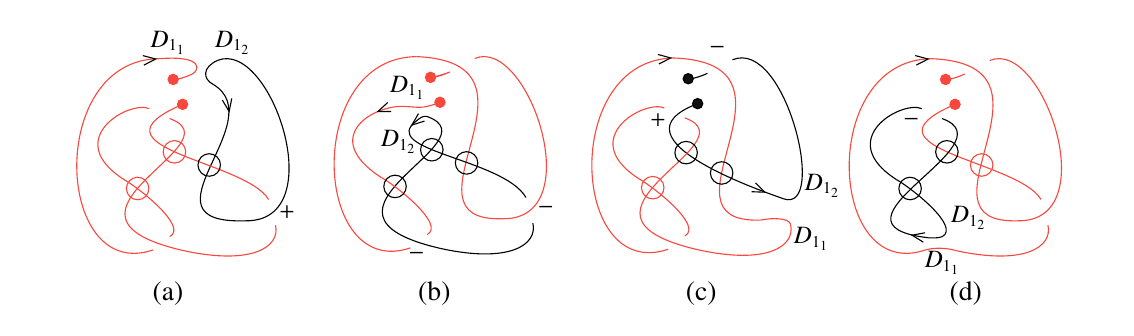
\begin{tikzpicture}[x=0.75pt,y=0.75pt,yscale=-1.0,xscale=1.0]
					\draw [color={rgb, 255:red, 248; green, 72; blue, 61 }  ,draw opacity=1 ]   (70.47,131.63) .. controls (23.34,147.68) and (18.73,40.05) .. (73.39,39.48) ;
					\draw    (99.49,51.86) .. controls (128.49,69.38) and (61,119.31) .. (114.94,117.58) ;
					\draw [color={rgb, 255:red, 248; green, 72; blue, 61 }  ,draw opacity=1 ]   (84.74,61.47) .. controls (35.72,82.58) and (115.23,88.54) .. (126.18,107.33) ;
					\draw    (114.94,117.58) .. controls (157.13,118.34) and (127.21,29.68) .. (101.5,40.34) ;
					\draw [color={rgb, 255:red, 248; green, 72; blue, 61 }  ,draw opacity=1 ]   (78.48,68.31) .. controls (112.41,80.5) and (10.37,114.64) .. (84.88,131.87) ;
					\draw [color={rgb, 255:red, 248; green, 72; blue, 61 }  ,draw opacity=1 ]   (68.69,63.53) .. controls (58.97,59.39) and (26.16,78.26) .. (56.53,97.73) ;
					\draw [color={rgb, 255:red, 248; green, 72; blue, 61 }  ,draw opacity=1 ]   (56.53,97.73) .. controls (63.82,101.87) and (87.47,120.43) .. (78.57,125.21) ;
					\draw [color={rgb, 255:red, 248; green, 72; blue, 61 }  ,draw opacity=1 ]   (84.88,131.87) .. controls (118.08,139.2) and (131.89,130.26) .. (129.51,119.71) ;
					\draw  [color={rgb, 255:red, 248; green, 72; blue, 61 }  ,draw opacity=1 ] (86.24,84.25) .. controls (86.29,87.24) and (83.91,89.71) .. (80.91,89.76) .. controls (77.92,89.81) and (75.45,87.43) .. (75.4,84.44) .. controls (75.35,81.45) and (77.73,78.98) .. (80.72,78.93) .. controls (83.72,78.87) and (86.18,81.26) .. (86.24,84.25) -- cycle ;
					\draw  [color={rgb, 255:red, 248; green, 72; blue, 61 }  ,draw opacity=1 ] (68.51,101.93) .. controls (68.56,104.92) and (66.18,107.39) .. (63.19,107.44) .. controls (60.2,107.49) and (57.73,105.11) .. (57.68,102.12) .. controls (57.62,99.12) and (60.01,96.66) .. (63,96.6) .. controls (65.99,96.55) and (68.46,98.93) .. (68.51,101.93) -- cycle ;
					\draw   (102.99,90.59) .. controls (103.04,93.59) and (100.66,96.05) .. (97.66,96.11) .. controls (94.67,96.16) and (92.2,93.77) .. (92.15,90.78) .. controls (92.1,87.79) and (94.48,85.32) .. (97.47,85.27) .. controls (100.47,85.22) and (102.93,87.6) .. (102.99,90.59) -- cycle ; 
					\draw [color={rgb, 255:red, 248; green, 72; blue, 61 }  ,draw opacity=1 ]   (80.2,49.47) .. controls (82.1,49.81) and (87.44,47.86) .. (89.45,46.85) ;
					\draw  [color={rgb, 255:red, 248; green, 72; blue, 61 }  ,draw opacity=1 ][fill={rgb, 255:red, 248; green, 72; blue, 61 }  ,fill opacity=1 ] (82.67,49.44) .. controls (82.65,48.07) and (81.53,46.98) .. (80.17,46.99) .. controls (78.81,47.01) and (77.71,48.13) .. (77.73,49.5) .. controls (77.74,50.87) and (78.86,51.96) .. (80.23,51.95) .. controls (81.59,51.93) and (82.68,50.81) .. (82.67,49.44) -- cycle ;
					\draw  [color={rgb, 255:red, 248; green, 72; blue, 61 }  ,draw opacity=1 ][fill={rgb, 255:red, 248; green, 72; blue, 61 }  ,fill opacity=1 ] (87.21,61.44) .. controls (87.2,60.08) and (86.08,58.98) .. (84.71,58.99) .. controls (83.35,59.01) and (82.26,60.13) .. (82.27,61.5) .. controls (82.29,62.87) and (83.4,63.97) .. (84.77,63.95) .. controls (86.13,63.93) and (87.23,62.81) .. (87.21,61.44) -- cycle ;
					\draw   (65.59,37.98) -- (71.77,39.64) -- (66.08,42.57) ;
					\draw [color={rgb, 255:red, 248; green, 72; blue, 61 }  ,draw opacity=1 ]   (194.47,130.63) .. controls (147.34,146.68) and (142.73,39.05) .. (197.39,38.48) ;
					\draw [color={rgb, 255:red, 248; green, 72; blue, 61 }  ,draw opacity=1 ]   (197.39,38.48) .. controls (266.78,41.21) and (185,118.31) .. (238.94,116.58) ;
					\draw    (197.74,69.19) .. controls (177.88,83.76) and (239.23,87.54) .. (250.18,106.33) ; 
					\draw [color={rgb, 255:red, 248; green, 72; blue, 61 }  ,draw opacity=1 ]   (238.94,116.58) .. controls (281.13,117.34) and (251.21,28.68) .. (225.5,39.34) ;
					\draw    (202.48,67.31) .. controls (236.41,79.5) and (134.37,113.64) .. (208.88,130.87) ;
					\draw [color={rgb, 255:red, 248; green, 72; blue, 61 }  ,draw opacity=1 ]   (192.69,62.53) .. controls (177.02,61) and (150.16,77.26) .. (180.53,96.73) ; 
					\draw [color={rgb, 255:red, 248; green, 72; blue, 61 }  ,draw opacity=1 ]   (180.53,96.73) .. controls (187.82,100.87) and (211.47,119.43) .. (202.57,124.21) ;
					\draw    (208.88,130.87) .. controls (242.08,138.2) and (255.89,129.26) .. (253.51,118.71) ;
					\draw   (210.24,83.25) .. controls (210.29,86.24) and (207.91,88.71) .. (204.91,88.76) .. controls (201.92,88.81) and (199.45,86.43) .. (199.4,83.44) .. controls (199.35,80.45) and (201.73,77.98) .. (204.72,77.93) .. controls (207.72,77.87) and (210.18,80.26) .. (210.24,83.25) -- cycle ;
					\draw   (192.51,100.93) .. controls (192.56,103.92) and (190.18,106.39) .. (187.19,106.44) .. controls (184.2,106.49) and (181.73,104.11) .. (181.68,101.12) .. controls (181.62,98.12) and (184.01,95.66) .. (187,95.6) .. controls (189.99,95.55) and (192.46,97.93) .. (192.51,100.93) -- cycle ;
					\draw   (226.99,89.59) .. controls (227.04,92.59) and (224.66,95.05) .. (221.66,95.11) .. controls (218.67,95.16) and (216.2,92.77) .. (216.15,89.78) .. controls (216.1,86.79) and (218.48,84.32) .. (221.47,84.27) .. controls (224.47,84.22) and (226.93,86.6) .. (226.99,89.59) -- cycle ;
					\draw [color={rgb, 255:red, 248; green, 72; blue, 61 }  ,draw opacity=1 ][fill={rgb, 255:red, 248; green, 72; blue, 61 }  ,fill opacity=1 ]   (204.2,48.47) .. controls (206.1,48.81) and (211.44,46.86) .. (213.45,45.85) ;
					\draw  [color={rgb, 255:red, 248; green, 72; blue, 61 }  ,draw opacity=1 ][fill={rgb, 255:red, 248; green, 72; blue, 61 }  ,fill opacity=1 ] (206.67,48.44) .. controls (206.65,47.07) and (205.53,45.98) .. (204.17,45.99) .. controls (202.81,46.01) and (201.71,47.13) .. (201.73,48.5) .. controls (201.74,49.87) and (202.86,50.96) .. (204.23,50.95) .. controls (205.59,50.93) and (206.68,49.81) .. (206.67,48.44) -- cycle ; 
					\draw  [color={rgb, 255:red, 248; green, 72; blue, 61 }  ,draw opacity=1 ][fill={rgb, 255:red, 248; green, 72; blue, 61 }  ,fill opacity=1 ] (211.21,60.44) .. controls (211.2,59.08) and (210.08,57.98) .. (208.71,57.99) .. controls (207.35,58.01) and (206.26,59.13) .. (206.27,60.5) .. controls (206.29,61.87) and (207.4,62.97) .. (208.77,62.95) .. controls (210.13,62.93) and (211.23,61.81) .. (211.21,60.44) -- cycle ;
					\draw   (185.24,64.9) -- (178.84,64.91) -- (183.57,60.6) ; 
					\draw [color={rgb, 255:red, 248; green, 72; blue, 61 }  ,draw opacity=1 ]   (318.63,131.3) .. controls (271.5,147.34) and (266.89,39.72) .. (321.55,39.14) ; 
					\draw [color={rgb, 255:red, 248; green, 72; blue, 61 }  ,draw opacity=1 ]   (321.55,39.14) .. controls (390.94,41.88) and (309.16,118.97) .. (363.1,117.25) ; 
					\draw    (332.9,61.14) .. controls (288.13,78.08) and (367.4,104.44) .. (374.34,107) ;
					\draw    (374.34,107) .. controls (395.77,114.26) and (375.37,29.35) .. (349.66,40.01) ; 
					\draw [color={rgb, 255:red, 248; green, 72; blue, 61 }  ,draw opacity=1 ]   (326.64,67.98) .. controls (360.57,80.16) and (258.53,114.3) .. (333.04,131.53) ;
					\draw [color={rgb, 255:red, 248; green, 72; blue, 61 }  ,draw opacity=1 ]   (316.85,63.2) .. controls (307.13,59.05) and (274.32,77.93) .. (304.69,97.39) ;
					\draw [color={rgb, 255:red, 248; green, 72; blue, 61 }  ,draw opacity=1 ]   (304.69,97.39) .. controls (311.98,101.54) and (335.63,120.09) .. (326.73,124.88) ; 
					\draw [color={rgb, 255:red, 248; green, 72; blue, 61 }  ,draw opacity=1 ]   (333.04,131.53) .. controls (366.24,138.87) and (380.05,129.92) .. (377.67,119.38) ;
					\draw   (332.76,84.64) .. controls (332.81,87.63) and (330.43,90.1) .. (327.44,90.15) .. controls (324.45,90.21) and (321.98,87.82) .. (321.93,84.83) .. controls (321.87,81.84) and (324.26,79.37) .. (327.25,79.32) .. controls (330.24,79.27) and (332.71,81.65) .. (332.76,84.64) -- cycle ;
					\draw  [color={rgb, 255:red, 248; green, 72; blue, 61 }  ,draw opacity=1 ] (316.67,101.53) .. controls (316.72,104.52) and (314.34,106.99) .. (311.35,107.04) .. controls (308.36,107.09) and (305.89,104.71) .. (305.84,101.72) .. controls (305.78,98.72) and (308.17,96.26) .. (311.16,96.2) .. controls (314.15,96.15) and (316.62,98.54) .. (316.67,101.53) -- cycle ;
					\draw   (349.88,94.44) .. controls (349.93,97.43) and (347.54,99.9) .. (344.55,99.95) .. controls (341.56,100.01) and (339.09,97.62) .. (339.04,94.63) .. controls (338.99,91.64) and (341.37,89.17) .. (344.36,89.12) .. controls (347.35,89.07) and (349.82,91.45) .. (349.88,94.44) -- cycle ;
					\draw    (328.36,49.14) .. controls (330.26,49.48) and (335.6,47.53) .. (337.61,46.52) ;
					\draw  [fill={rgb, 255:red, 17; green, 16; blue, 16 }  ,fill opacity=1 ] (330.83,49.11) .. controls (330.81,47.74) and (329.7,46.64) .. (328.33,46.66) .. controls (326.97,46.67) and (325.87,47.79) .. (325.89,49.16) .. controls (325.9,50.53) and (327.02,51.63) .. (328.39,51.61) .. controls (329.75,51.6) and (330.84,50.48) .. (330.83,49.11) -- cycle ;
					\draw  [fill={rgb, 255:red, 17; green, 16; blue, 16 }  ,fill opacity=1 ] (335.37,61.11) .. controls (335.36,59.74) and (334.24,58.65) .. (332.87,58.66) .. controls (331.51,58.68) and (330.42,59.8) .. (330.43,61.17) .. controls (330.45,62.54) and (331.57,63.63) .. (332.93,63.62) .. controls (334.29,63.6) and (335.39,62.48) .. (335.37,61.11) -- cycle ;
					\draw   (313.75,37.45) -- (319.93,39.11) -- (314.24,42.04) ;
					\draw [color={rgb, 255:red, 248; green, 72; blue, 61 }  ,draw opacity=1 ]   (442.63,131.63) .. controls (395.5,147.68) and (390.89,40.05) .. (445.55,39.48) ; 
					\draw [color={rgb, 255:red, 248; green, 72; blue, 61 }  ,draw opacity=1 ]   (445.55,39.48) .. controls (514.94,42.21) and (433.16,119.31) .. (487.1,117.58) ;
					\draw [color={rgb, 255:red, 248; green, 72; blue, 61 }  ,draw opacity=1 ]   (456.9,61.47) .. controls (407.88,82.58) and (487.39,88.54) .. (498.34,107.33) ; 
					\draw [color={rgb, 255:red, 248; green, 72; blue, 61 }  ,draw opacity=1 ]   (487.1,117.58) .. controls (529.29,118.34) and (499.37,29.68) .. (473.66,40.34) ;
					\draw    (450.64,68.31) .. controls (484.57,80.5) and (387.36,119.36) .. (444.16,125.76) ;
					\draw    (440.85,63.53) .. controls (431.13,59.39) and (398.32,78.26) .. (428.69,97.73) ;
					\draw    (428.69,97.73) .. controls (435.98,101.87) and (459.63,120.43) .. (450.73,125.21) ;
					\draw [color={rgb, 255:red, 248; green, 72; blue, 61 }  ,draw opacity=1 ]   (457.04,131.87) .. controls (490.24,139.2) and (504.05,130.26) .. (501.67,119.71) ;
					\draw   (458.4,84.25) .. controls (458.45,87.24) and (456.07,89.71) .. (453.07,89.76) .. controls (450.08,89.81) and (447.61,87.43) .. (447.56,84.44) .. controls (447.51,81.45) and (449.89,78.98) .. (452.89,78.93) .. controls (455.88,78.87) and (458.35,81.26) .. (458.4,84.25) -- cycle ;
					\draw   (440.67,101.93) .. controls (440.72,104.92) and (438.34,107.39) .. (435.35,107.44) .. controls (432.36,107.49) and (429.89,105.11) .. (429.84,102.12) .. controls (429.78,99.12) and (432.17,96.66) .. (435.16,96.6) .. controls (438.15,96.55) and (440.62,98.93) .. (440.67,101.93) -- cycle ;
					\draw  [color={rgb, 255:red, 248; green, 72; blue, 61 }  ,draw opacity=1 ] (475.15,90.59) .. controls (475.2,93.59) and (472.82,96.05) .. (469.82,96.11) .. controls (466.83,96.16) and (464.36,93.77) .. (464.31,90.78) .. controls (464.26,87.79) and (466.64,85.32) .. (469.64,85.27) .. controls (472.63,85.22) and (475.1,87.6) .. (475.15,90.59) -- cycle ;
					\draw [color={rgb, 255:red, 248; green, 72; blue, 61 }  ,draw opacity=1 ]   (452.36,49.47) .. controls (454.26,49.81) and (459.6,47.86) .. (461.61,46.85) ;
					\draw  [color={rgb, 255:red, 248; green, 72; blue, 61 }  ,draw opacity=1 ][fill={rgb, 255:red, 248; green, 72; blue, 61 }  ,fill opacity=1 ] (454.83,49.44) .. controls (454.81,48.07) and (453.7,46.98) .. (452.33,46.99) .. controls (450.97,47.01) and (449.87,48.13) .. (449.89,49.5) .. controls (449.9,50.87) and (451.02,51.96) .. (452.39,51.95) .. controls (453.75,51.93) and (454.84,50.81) .. (454.83,49.44) -- cycle ; 
					\draw  [color={rgb, 255:red, 248; green, 72; blue, 61 }  ,draw opacity=1 ][fill={rgb, 255:red, 248; green, 72; blue, 61 }  ,fill opacity=1 ] (459.37,61.44) .. controls (459.36,60.08) and (458.24,58.98) .. (456.87,58.99) .. controls (455.51,59.01) and (454.42,60.13) .. (454.43,61.5) .. controls (454.45,62.87) and (455.57,63.97) .. (456.93,63.95) .. controls (458.29,63.93) and (459.39,62.81) .. (459.37,61.44) -- cycle ;
					\draw   (437.75,37.98) -- (443.93,39.64) -- (438.24,42.57) ;
					\draw [color={rgb, 255:red, 248; green, 72; blue, 61 }  ,draw opacity=1 ]   (73.39,39.48) .. controls (95.76,37.75) and (92.53,45.36) .. (89.45,46.85) ;
					\draw    (101.5,40.34) .. controls (94.2,43.64) and (94.43,49.29) .. (99.49,51.86) ;
					\draw   (108.44,58.64) -- (107.15,64.9) -- (103.89,59.4) ;
					\draw    (197.74,69.19) .. controls (198.44,68.6) and (200.62,66.69) .. (202.48,67.31) ;
					\draw [color={rgb, 255:red, 248; green, 72; blue, 61 }  ,draw opacity=1 ]   (192.69,62.53) .. controls (198.72,63) and (199.93,63.1) .. (202.84,62.4) .. controls (205.74,61.7) and (208.11,60.76) .. (208.74,60.47) ;
					\draw   (201.3,69.52) -- (195.2,71.46) -- (198.41,65.93) ;
					\draw [color={rgb, 255:red, 248; green, 72; blue, 61 }  ,draw opacity=1 ]   (363.1,117.25) .. controls (369.04,116.02) and (377.22,116.2) .. (377.67,119.38) ;
					\draw   (360.74,99.32) -- (365.3,103.81) -- (358.91,103.56) ; 
					\draw    (444.16,125.76) .. controls (445.82,125.91) and (449.35,125.91) .. (450.73,125.21) ; 
					\draw [color={rgb, 255:red, 248; green, 72; blue, 61 }  ,draw opacity=1 ]   (442.63,131.63) .. controls (447.01,130.29) and (453.66,130.75) .. (457.04,131.87) ;
					\draw   (441.62,127.88) -- (436.18,124.51) -- (442.47,123.35) ;
					\draw (67.8,24.82) node [anchor=north west][inner sep=0.75pt]  [font=\small]  {$D_{1_1}$};
					\draw (98.8,24.8) node [anchor=north west][inner sep=0.75pt]  [font=\small]  {$D_{1_2}$};
					\draw (130,109) node [anchor=north west][inner sep=0.75pt]  [font=\small]  {$+$};
					\draw (183.11,46.44) node [anchor=north west][inner sep=0.75pt]  [font=\small]  {$D_{1_1}$};
					\draw (178.85,72.66) node [anchor=north west][inner sep=0.75pt]  [font=\small]  {$D_{1_2}$};
					\draw (254.7,106.55) node [anchor=north west][inner sep=0.75pt]  [font=\small]  {$-$};
					\draw (192.33,129.02) node [anchor=north west][inner sep=0.75pt]  [font=\small]  {$-$};
					\draw (308.76,64.93) node [anchor=north west][inner sep=0.75pt]  [font=\small]  {$+$};
					\draw (337.3,29.39) node [anchor=north west][inner sep=0.75pt]  [font=\small]  {$-$};
					\draw (377.67,119.38) node [anchor=north west][inner sep=0.75pt]  [font=\small]  {$D_{1_1}$};
					\draw (383.03,93.67) node [anchor=north west][inner sep=0.75pt]  [font=\small]  {$D_{1_2}$};
					\draw (440.75,130.88) node [anchor=north west][inner sep=0.75pt]  [font=\small]  {$D_{1_1}$};
					\draw (453.49,109.32) node [anchor=north west][inner sep=0.75pt]  [font=\small]  {$D_{1_2}$};
					\draw (430.7,64.12) node [anchor=north west][inner sep=0.75pt]  [font=\small]  {$-$};
					\draw (69,145.85) node [anchor=north west][inner sep=0.75pt]   [align=left] {(a)};
					\draw (453,145.85) node [anchor=north west][inner sep=0.75pt]   [align=left] {(d)};
					\draw (326,145.85) node [anchor=north west][inner sep=0.75pt]   [align=left] {(c)};
					\draw (197,145.85) node [anchor=north west][inner sep=0.75pt]   [align=left] {(b)};
				\end{tikzpicture}
			\caption{(a)--(d): Diagrams obtained by orientation-preserving smoothing at classical crossings $c_1$, $c_2$, $c_3$ and $c_4$ in $D_1$.} \label{fig516}
		\end{figure}
		
		\begin{figure}[!ht]
			\centering
				\tikzset{every picture/.style={line width=1.0pt}} 
				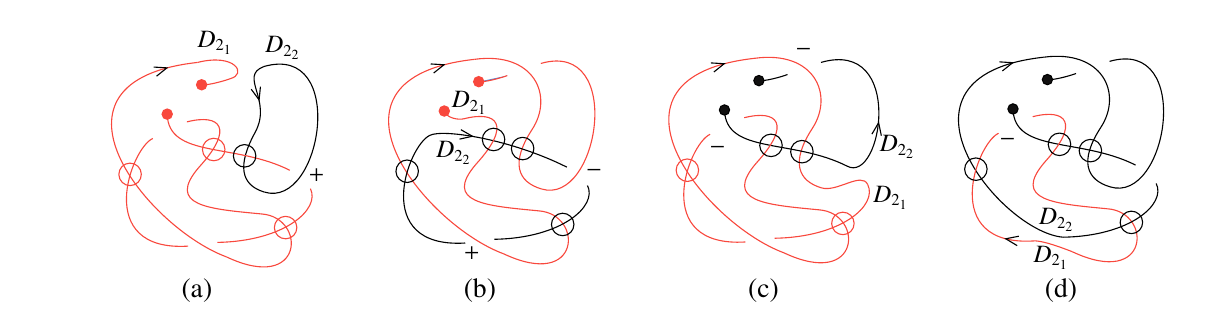
\begin{tikzpicture}[x=0.75pt,y=0.75pt,yscale=-1.0,xscale=1.0]
					\draw [color={rgb, 255:red, 248; green, 72; blue, 61 }  ,draw opacity=1 ]   (90.98,266.63) .. controls (53.01,252.62) and (-4.58,181.96) .. (76.98,172.92) ;
					\draw    (108.89,174.91) .. controls (96.65,179.65) and (113.32,190.98) .. (104.71,206.68) .. controls (96.1,222.38) and (97.7,231.96) .. (109.19,235.38) ;
					\draw [color={rgb, 255:red, 248; green, 72; blue, 61 }  ,draw opacity=1 ]   (62.38,197.83) .. controls (62.93,219.3) and (94.9,211.51) .. (121.43,224.87) ;
					\draw    (109.19,235.38) .. controls (136.88,243.8) and (149.67,163.14) .. (108.89,174.91) ;
					\draw [color={rgb, 255:red, 248; green, 72; blue, 61 }  ,draw opacity=1 ]   (71.87,201.56) .. controls (87.99,197.46) and (94.86,204.54) .. (77.84,223.24) ;
					\draw [color={rgb, 255:red, 248; green, 72; blue, 61 }  ,draw opacity=1 ]   (55.42,209.55) .. controls (44.87,214.35) and (26.49,264.24) .. (72.47,261.42) ;
					\draw [color={rgb, 255:red, 248; green, 72; blue, 61 }  ,draw opacity=1 ]   (90.98,266.63) .. controls (128.6,284.37) and (129.49,247.58) .. (108,245.94) ;
					\draw [color={rgb, 255:red, 248; green, 72; blue, 61 }  ,draw opacity=1 ]   (77.84,223.24) .. controls (61.42,242.2) and (82.62,243.48) .. (108,245.94) ;
					\draw [color={rgb, 255:red, 248; green, 72; blue, 61 }  ,draw opacity=1 ]   (78.96,183.68) .. controls (81.8,184.07) and (89.75,181.88) .. (92.74,180.75) ;
					\draw  [color={rgb, 255:red, 248; green, 72; blue, 61 }  ,draw opacity=1 ][fill={rgb, 255:red, 248; green, 72; blue, 61 }  ,fill opacity=1 ] (81.43,183.65) .. controls (81.41,182.28) and (80.3,181.19) .. (78.93,181.2) .. controls (77.57,181.22) and (76.47,182.34) .. (76.49,183.71) .. controls (76.5,185.08) and (77.62,186.18) .. (78.99,186.16) .. controls (80.35,186.14) and (81.44,185.02) .. (81.43,183.65) -- cycle ;
					\draw  [color={rgb, 255:red, 248; green, 72; blue, 61 }  ,draw opacity=1 ][fill={rgb, 255:red, 248; green, 72; blue, 61 }  ,fill opacity=1 ] (64.85,197.8) .. controls (64.83,196.43) and (63.71,195.34) .. (62.35,195.35) .. controls (60.98,195.37) and (59.89,196.49) .. (59.9,197.86) .. controls (59.92,199.23) and (61.04,200.32) .. (62.4,200.31) .. controls (63.77,200.29) and (64.86,199.17) .. (64.85,197.8) -- cycle ;
					\draw   (55.85,175.15) -- (62.23,175.54) -- (57.25,179.54) ;
					\draw [color={rgb, 255:red, 248; green, 72; blue, 61 }  ,draw opacity=1 ]   (86.5,259.62) .. controls (118.74,259.11) and (136.34,243.71) .. (131.37,233.72) ;
					\draw  [color={rgb, 255:red, 248; green, 72; blue, 61 }  ,draw opacity=1 ] (49.91,226.75) .. controls (49.97,229.74) and (47.58,232.21) .. (44.59,232.26) .. controls (41.6,232.31) and (39.13,229.93) .. (39.08,226.94) .. controls (39.03,223.95) and (41.41,221.48) .. (44.4,221.43) .. controls (47.39,221.37) and (49.86,223.76) .. (49.91,226.75) -- cycle ;
					\draw   (105.09,217.82) .. controls (105.14,220.81) and (102.76,223.28) .. (99.77,223.33) .. controls (96.78,223.38) and (94.31,221) .. (94.26,218.01) .. controls (94.2,215.02) and (96.59,212.55) .. (99.58,212.5) .. controls (102.57,212.44) and (105.04,214.83) .. (105.09,217.82) -- cycle ;
					\draw  [color={rgb, 255:red, 248; green, 72; blue, 61 }  ,draw opacity=1 ] (124.84,252.39) .. controls (124.89,255.38) and (122.51,257.85) .. (119.52,257.9) .. controls (116.53,257.96) and (114.06,255.57) .. (114.01,252.58) .. controls (113.95,249.59) and (116.34,247.12) .. (119.33,247.07) .. controls (122.32,247.02) and (124.79,249.4) .. (124.84,252.39) -- cycle ;
					\draw  [color={rgb, 255:red, 248; green, 72; blue, 61 }  ,draw opacity=1 ] (90.2,214.78) .. controls (90.25,217.77) and (87.87,220.24) .. (84.88,220.29) .. controls (81.88,220.34) and (79.42,217.96) .. (79.36,214.97) .. controls (79.31,211.98) and (81.7,209.51) .. (84.69,209.46) .. controls (87.68,209.4) and (90.15,211.79) .. (90.2,214.78) -- cycle ;
					\draw [color={rgb, 255:red, 248; green, 72; blue, 61 }  ,draw opacity=1 ]   (224.48,265.13) .. controls (186.51,251.12) and (128.92,180.46) .. (210.48,171.42) ;
					\draw [color={rgb, 255:red, 248; green, 72; blue, 61 }  ,draw opacity=1 ]   (210.48,171.42) .. controls (239.11,167.52) and (248.8,188.93) .. (238.21,205.18) .. controls (227.63,221.44) and (231.2,230.46) .. (242.69,233.88) ;
					\draw    (188.92,208.05) .. controls (195.32,204.79) and (228.4,210.01) .. (254.93,223.37) ;
					\draw [color={rgb, 255:red, 248; green, 72; blue, 61 }  ,draw opacity=1 ]   (242.69,233.88) .. controls (270.38,242.3) and (283.17,161.64) .. (242.39,173.41) ;
					\draw [color={rgb, 255:red, 248; green, 72; blue, 61 }  ,draw opacity=1 ]   (205.37,200.06) .. controls (221.49,195.96) and (228.36,203.04) .. (211.34,221.74) ;
					\draw    (188.92,208.05) .. controls (178.37,212.85) and (159.99,262.74) .. (205.97,259.92) ;
					\draw [color={rgb, 255:red, 248; green, 72; blue, 61 }  ,draw opacity=1 ]   (224.48,265.13) .. controls (262.1,282.87) and (262.99,246.08) .. (241.5,244.44) ;
					\draw [color={rgb, 255:red, 248; green, 72; blue, 61 }  ,draw opacity=1 ]   (211.34,221.74) .. controls (194.92,240.7) and (216.12,241.98) .. (241.5,244.44) ;
					\draw [color={rgb, 255:red, 248; green, 72; blue, 61 }  ,draw opacity=1 ][fill={rgb, 255:red, 74; green, 144; blue, 226 }  ,fill opacity=1 ]   (212.46,182.18) .. controls (215.3,182.57) and (223.25,180.38) .. (226.24,179.25) ;
					\draw  [color={rgb, 255:red, 248; green, 72; blue, 61 }  ,draw opacity=1 ][fill={rgb, 255:red, 248; green, 72; blue, 61 }  ,fill opacity=1 ] (214.93,182.15) .. controls (214.91,180.78) and (213.8,179.69) .. (212.43,179.7) .. controls (211.07,179.72) and (209.97,180.84) .. (209.99,182.21) .. controls (210,183.58) and (211.12,184.68) .. (212.49,184.66) .. controls (213.85,184.64) and (214.94,183.52) .. (214.93,182.15) -- cycle ; 
					\draw  [color={rgb, 255:red, 248; green, 72; blue, 61 }  ,draw opacity=1 ][fill={rgb, 255:red, 248; green, 72; blue, 61 }  ,fill opacity=1 ] (198.35,196.3) .. controls (198.33,194.93) and (197.21,193.84) .. (195.85,193.85) .. controls (194.48,193.87) and (193.39,194.99) .. (193.4,196.36) .. controls (193.42,197.73) and (194.54,198.82) .. (195.9,198.81) .. controls (197.27,198.79) and (198.36,197.67) .. (198.35,196.3) -- cycle ;
					\draw   (189.35,173.65) -- (195.73,174.04) -- (190.75,178.04) ;
					\draw    (220,258.12) .. controls (252.24,257.61) and (269.84,242.21) .. (264.87,232.22) ;
					\draw   (183.41,225.25) .. controls (183.47,228.24) and (181.08,230.71) .. (178.09,230.76) .. controls (175.1,230.81) and (172.63,228.43) .. (172.58,225.44) .. controls (172.53,222.45) and (174.91,219.98) .. (177.9,219.93) .. controls (180.89,219.87) and (183.36,222.26) .. (183.41,225.25) -- cycle ;
					\draw   (239.04,214.32) .. controls (239.09,217.31) and (236.71,219.78) .. (233.71,219.83) .. controls (230.72,219.88) and (228.25,217.5) .. (228.2,214.51) .. controls (228.15,211.52) and (230.53,209.05) .. (233.52,209) .. controls (236.52,208.94) and (238.98,211.33) .. (239.04,214.32) -- cycle ;
					\draw   (258.34,250.89) .. controls (258.39,253.88) and (256.01,256.35) .. (253.02,256.4) .. controls (250.03,256.46) and (247.56,254.07) .. (247.51,251.08) .. controls (247.45,248.09) and (249.84,245.62) .. (252.83,245.57) .. controls (255.82,245.52) and (258.29,247.9) .. (258.34,250.89) -- cycle ;
					\draw   (225.03,209.95) .. controls (225.08,212.94) and (222.7,215.41) .. (219.71,215.46) .. controls (216.72,215.51) and (214.25,213.13) .. (214.2,210.14) .. controls (214.15,207.14) and (216.53,204.68) .. (219.52,204.62) .. controls (222.51,204.57) and (224.98,206.95) .. (225.03,209.95) -- cycle ;
					\draw [color={rgb, 255:red, 248; green, 72; blue, 61 }  ,draw opacity=1 ]   (359.48,264.63) .. controls (321.51,250.62) and (263.92,179.96) .. (345.48,170.92) ;
					\draw [color={rgb, 255:red, 248; green, 72; blue, 61 }  ,draw opacity=1 ]   (345.48,170.92) .. controls (374.11,167.02) and (383.8,188.43) .. (373.21,204.68) .. controls (362.63,220.94) and (366.2,229.96) .. (377.69,233.38) ;
					\draw    (330.88,195.83) .. controls (331.43,217.3) and (363.4,209.51) .. (389.93,222.87) ;
					\draw    (389.93,222.87) .. controls (406.76,231.93) and (418.17,161.14) .. (377.39,172.91) ;
					\draw [color={rgb, 255:red, 248; green, 72; blue, 61 }  ,draw opacity=1 ]   (340.37,199.56) .. controls (356.49,195.46) and (363.36,202.54) .. (346.34,221.24) ;
					\draw [color={rgb, 255:red, 248; green, 72; blue, 61 }  ,draw opacity=1 ]   (323.92,207.55) .. controls (313.37,212.35) and (294.99,262.24) .. (340.97,259.42) ;
					\draw [color={rgb, 255:red, 248; green, 72; blue, 61 }  ,draw opacity=1 ]   (359.48,264.63) .. controls (397.1,282.37) and (397.99,245.58) .. (376.5,243.94) ;
					\draw [color={rgb, 255:red, 248; green, 72; blue, 61 }  ,draw opacity=1 ]   (346.34,221.24) .. controls (329.92,240.2) and (351.12,241.48) .. (376.5,243.94) ;
					\draw    (347.46,181.68) .. controls (350.3,182.07) and (358.25,179.88) .. (361.24,178.75) ;
					\draw  [fill={rgb, 255:red, 17; green, 16; blue, 16 }  ,fill opacity=1 ] (349.93,181.65) .. controls (349.91,180.28) and (348.8,179.19) .. (347.43,179.2) .. controls (346.07,179.22) and (344.97,180.34) .. (344.99,181.71) .. controls (345,183.08) and (346.12,184.18) .. (347.49,184.16) .. controls (348.85,184.14) and (349.94,183.02) .. (349.93,181.65) -- cycle ;
					\draw  [fill={rgb, 255:red, 17; green, 16; blue, 16 }  ,fill opacity=1 ] (333.35,195.8) .. controls (333.33,194.43) and (332.21,193.34) .. (330.85,193.35) .. controls (329.48,193.37) and (328.39,194.49) .. (328.4,195.86) .. controls (328.42,197.23) and (329.54,198.32) .. (330.9,198.31) .. controls (332.27,198.29) and (333.36,197.17) .. (333.35,195.8) -- cycle ;
					\draw   (324.35,173.15) -- (330.73,173.54) -- (325.75,177.54) ;
					\draw [color={rgb, 255:red, 248; green, 72; blue, 61 }  ,draw opacity=1 ]   (355,257.62) .. controls (387.24,257.11) and (404.84,241.71) .. (399.87,231.72) ;
					\draw  [color={rgb, 255:red, 248; green, 72; blue, 61 }  ,draw opacity=1 ] (318.41,224.75) .. controls (318.47,227.74) and (316.08,230.21) .. (313.09,230.26) .. controls (310.1,230.31) and (307.63,227.93) .. (307.58,224.94) .. controls (307.53,221.95) and (309.91,219.48) .. (312.9,219.43) .. controls (315.89,219.37) and (318.36,221.76) .. (318.41,224.75) -- cycle ;
					\draw   (373.59,215.82) .. controls (373.64,218.81) and (371.26,221.28) .. (368.27,221.33) .. controls (365.28,221.38) and (362.81,219) .. (362.76,216.01) .. controls (362.7,213.02) and (365.09,210.55) .. (368.08,210.5) .. controls (371.07,210.44) and (373.54,212.83) .. (373.59,215.82) -- cycle ;
					\draw  [color={rgb, 255:red, 248; green, 72; blue, 61 }  ,draw opacity=1 ] (393.34,250.39) .. controls (393.39,253.38) and (391.01,255.85) .. (388.02,255.9) .. controls (385.03,255.96) and (382.56,253.57) .. (382.51,250.58) .. controls (382.45,247.59) and (384.84,245.12) .. (387.83,245.07) .. controls (390.82,245.02) and (393.29,247.4) .. (393.34,250.39) -- cycle ;
					\draw   (358.7,212.78) .. controls (358.75,215.77) and (356.37,218.24) .. (353.38,218.29) .. controls (350.38,218.34) and (347.92,215.96) .. (347.86,212.97) .. controls (347.81,209.98) and (350.2,207.51) .. (353.19,207.46) .. controls (356.18,207.4) and (358.65,209.79) .. (358.7,212.78) -- cycle ;
					\draw    (494,257.12) .. controls (463.57,254.54) and (402.92,179.46) .. (484.48,170.42) ;
					\draw    (484.48,170.42) .. controls (513.11,166.52) and (522.8,187.93) .. (512.21,204.18) .. controls (501.63,220.44) and (505.2,229.46) .. (516.69,232.88) ;
					\draw    (469.88,195.33) .. controls (470.43,216.8) and (502.4,209.01) .. (528.93,222.37) ;
					\draw    (516.69,232.88) .. controls (544.38,241.3) and (557.17,160.64) .. (516.39,172.41) ;
					\draw [color={rgb, 255:red, 248; green, 72; blue, 61 }  ,draw opacity=1 ]   (479.37,199.06) .. controls (495.49,194.96) and (502.36,202.04) .. (485.34,220.74) ;
					\draw [color={rgb, 255:red, 248; green, 72; blue, 61 }  ,draw opacity=1 ]   (462.92,207.05) .. controls (452.37,211.85) and (433.99,261.74) .. (479.97,258.92) ;
					\draw [color={rgb, 255:red, 248; green, 72; blue, 61 }  ,draw opacity=1 ]   (498.48,264.13) .. controls (536.1,281.87) and (536.99,245.08) .. (515.5,243.44) ;
					\draw [color={rgb, 255:red, 248; green, 72; blue, 61 }  ,draw opacity=1 ]   (485.34,220.74) .. controls (468.92,239.7) and (490.12,240.98) .. (515.5,243.44) ;
					\draw    (486.46,181.18) .. controls (489.3,181.57) and (497.25,179.38) .. (500.24,178.25) ;
					\draw  [fill={rgb, 255:red, 17; green, 16; blue, 16 }  ,fill opacity=1 ] (488.93,181.15) .. controls (488.91,179.78) and (487.8,178.69) .. (486.43,178.7) .. controls (485.07,178.72) and (483.97,179.84) .. (483.99,181.21) .. controls (484,182.58) and (485.12,183.68) .. (486.49,183.66) .. controls (487.85,183.64) and (488.94,182.52) .. (488.93,181.15) -- cycle ;
					\draw  [fill={rgb, 255:red, 17; green, 16; blue, 16 }  ,fill opacity=1 ] (472.35,195.3) .. controls (472.33,193.93) and (471.21,192.84) .. (469.85,192.85) .. controls (468.48,192.87) and (467.39,193.99) .. (467.4,195.36) .. controls (467.42,196.73) and (468.54,197.82) .. (469.9,197.81) .. controls (471.27,197.79) and (472.36,196.67) .. (472.35,195.3) -- cycle ;
					\draw   (463.35,172.65) -- (469.73,173.04) -- (464.75,177.04) ;
					\draw    (494,257.12) .. controls (526.24,256.61) and (543.84,241.21) .. (538.87,231.22) ;
					\draw   (457.41,224.25) .. controls (457.47,227.24) and (455.08,229.71) .. (452.09,229.76) .. controls (449.1,229.81) and (446.63,227.43) .. (446.58,224.44) .. controls (446.53,221.45) and (448.91,218.98) .. (451.9,218.93) .. controls (454.89,218.87) and (457.36,221.26) .. (457.41,224.25) -- cycle ;
					\draw   (512.59,215.32) .. controls (512.64,218.31) and (510.26,220.78) .. (507.27,220.83) .. controls (504.28,220.88) and (501.81,218.5) .. (501.76,215.51) .. controls (501.7,212.52) and (504.09,210.05) .. (507.08,210) .. controls (510.07,209.94) and (512.54,212.33) .. (512.59,215.32) -- cycle ;
					\draw   (532.34,249.89) .. controls (532.39,252.88) and (530.01,255.35) .. (527.02,255.4) .. controls (524.03,255.46) and (521.56,253.07) .. (521.51,250.08) .. controls (521.45,247.09) and (523.84,244.62) .. (526.83,244.57) .. controls (529.82,244.52) and (532.29,246.9) .. (532.34,249.89) -- cycle ;
					\draw   (497.7,212.28) .. controls (497.75,215.27) and (495.37,217.74) .. (492.38,217.79) .. controls (489.38,217.84) and (486.92,215.46) .. (486.86,212.47) .. controls (486.81,209.48) and (489.2,207.01) .. (492.19,206.96) .. controls (495.18,206.9) and (497.65,209.29) .. (497.7,212.28) -- cycle ;
					\draw [color={rgb, 255:red, 248; green, 72; blue, 61 }  ,draw opacity=1 ]   (76.98,172.92) .. controls (95.32,168.31) and (100.99,178.65) .. (92.74,180.75) ;
					\draw   (107.3,184.6) -- (106.65,190.96) -- (102.85,185.82) ;
					\draw [color={rgb, 255:red, 248; green, 72; blue, 61 }  ,draw opacity=1 ]   (195.88,196.33) .. controls (196.87,199.68) and (202.65,200.79) .. (205.37,200.06) ;
					\draw   (203.88,205.32) -- (209.44,208.48) -- (203.2,209.88) ;
					\draw [color={rgb, 255:red, 248; green, 72; blue, 61 }  ,draw opacity=1 ]   (377.69,233.38) .. controls (385.06,235.58) and (396.91,225.42) .. (399.87,231.72) ;
					\draw   (401.9,207.47) -- (405.14,201.96) -- (406.45,208.22) ;
					\draw [color={rgb, 255:red, 248; green, 72; blue, 61 }  ,draw opacity=1 ]   (479.97,258.92) .. controls (484.9,258.6) and (497.9,263.94) .. (498.48,264.13) ;
					\draw   (471.9,261.18) -- (466.41,257.89) -- (472.68,256.64) ;
					\draw (75.47,156.44) node [anchor=north west][inner sep=0.75pt]  [font=\small]  {$D_{2_1}$};
					\draw (108.13,159.09) node [anchor=north west][inner sep=0.75pt]  [font=\small]  {$D_{2_2}$};
					\draw (129.22,222.83) node [anchor=north west][inner sep=0.75pt]  [font=\small]  {$+$};
					\draw (198.02,185.68) node [anchor=north west][inner sep=0.75pt]  [font=\small]  {$D_{2_1}$};
					\draw (190.47,209.56) node [anchor=north west][inner sep=0.75pt]  [font=\small]  {$D_{2_2}$};
					\draw (204,260.27) node [anchor=north west][inner sep=0.75pt]  [font=\small]  {$+$};
					\draw (262.89,220.56) node [anchor=north west][inner sep=0.75pt]  [font=\small]  {$-$};
					\draw (401.07,231.16) node [anchor=north west][inner sep=0.75pt]  [font=\small]  {$D_{2_1}$};
					\draw (404.2,206.89) node [anchor=north west][inner sep=0.75pt]  [font=\small]  {$D_{2_2}$};
					\draw (322.39,209.19) node [anchor=north west][inner sep=0.75pt]  [font=\small]  {$-$};
					\draw (363.89,162.19) node [anchor=north west][inner sep=0.75pt]  [font=\small]  {$-$};
					\draw (478.24,260) node [anchor=north west][inner sep=0.75pt]  [font=\small]  {$D_{2_1}$};
					\draw (480.87,241.89) node [anchor=north west][inner sep=0.75pt]  [font=\small]  {$D_{2_2}$};
					\draw (462.17,205.34) node [anchor=north west][inner sep=0.75pt]  [font=\small]  {$-$};
					\draw (68,275.88) node [anchor=north west][inner sep=0.75pt]   [align=left] {(a)};
					\draw (484,275.88) node [anchor=north west][inner sep=0.75pt]   [align=left] {(d)};
					\draw (341,275.88) node [anchor=north west][inner sep=0.75pt]   [align=left] {(c)};
					\draw (204,275.88) node [anchor=north west][inner sep=0.75pt]   [align=left] {(b)};
				\end{tikzpicture}
			\caption{(a)--(d): Diagrams obtained by orientation-preserving smoothing at classical crossings $c_1$, $c_2$, $c_3$ and $c_4$ in $D_2$.} \label{fig517}
		\end{figure}
		Combining the above results, we obtain that $\mathbf{P}_{K_1}(x,y)= \mathbf{P}_{K_2}(x,y)$. 
	}
\end{example}

\begin{thebibliography}{99}
\bibitem[Che]{Che} Z.~Cheng, \textit{The chord index, its definitions, applications, and generalizations}. Canadian Journal of Mathematics, 2021, 73(3): 597--621.
\bibitem[FK]{FK} L.~C.~Folwaczny and L.~H.~Kauffman, \textit{A linking number definition of the affine index polynomial and applications}, Journal of Knot Theory and Its Ramifications, 2013, 22(12): 1341004.
\bibitem[FLV]{FLV} W.~Feng, F.~Li, A.~Vesnin, \textit{A three-variable transcendental invariant of planar knotoids via Gauss diagrams}. Mediterranean Journal of Mathematics, 2025, 22(4): 99.
\bibitem[GK]{GK} N.~G\"{u}g\"{u}mc\"{u}, L.~Kauffman, \textit{New invariants of knotoids}. European Journal of Combinatorics, 2017, 65: 186--229.
\bibitem[Hen]{Hen} A.~Henrich, \textit{A sequence of degree one Vassiliev invariants for virtual knots}. Journal of Knot Theory and its Ramifications, 2010, 19(04): 461--487.
\bibitem[Lee]{Lee} K.~Lee, \textit{Index polynomial invariants of virtual knots using invariants for flat virtual knots}. Journal of Knot Theory and Its Ramifications 2023, 32(02): 2350015.
\bibitem[Man]{Man} V.\,O.~Manturov, \textit{Parity in knot theory}. Sbornik: Mathematics, 2010, 201(5): 693-733.
\end{thebibliography}
\end{document}
